% =========================================================================
%        LaTeX Template for PhD Thesis
% =========================================================================

%\RequirePackage[l2tabu, orthodox]{nag} % display more warnings

\documentclass{sokendai_thesis} % for final version
%\documentclass[todo]{sokendai_thesis} % print todo notes (generated by this command: \mytodo[inline]{this is just a todo note})


% =====================================================
%  User-defined Commands
% =====================================================

\newcommand{\Order}{\mathit{O}} % for computational complexity


% =====================================================
%  Thesis Info
% =====================================================

\title{A Study on Portable Load Balancer for Container Clusters}
\author{Kimitoshi Takahashi}
\date{March 2019}
\crest{Crest/sokendai_crest.pdf} % comment out if you don't have a crest.
%\keywords{Latex Template, Sokendai, PhD Thesis} % for PDF meta-info

\usepackage{xcolor}
\definecolor{mygray}{rgb}{0.95,0.99,0.99}

% =====================================================
%  Others
% =====================================================

% Typeset only specified chapters
%\includeonly{Manuscript/Introduction/introduction}


% =====================================================
%  Front Matter
% =====================================================

\begin{document}

\frontmatter
\maketitle

% \listoftodos

\chapter*{Acknowledgments}

\added{
First and foremost, I would like to express my sincere gratitude to my advisor Prof. Kento Aida for the continuous support of my Ph.D. study, for his patience, motivation, enthusiasm, and immense knowledge.
His guidance helped me in all the time of research and writing of this thesis.
I could not have imagined having a better advisor and mentor for my Ph.D. study.
}

\added{
Besides my advisor, I would like to sincerely thank the rest of my thesis committee: Prof. Atsuko Takefusa, Prof. Michihiro Koibuchi, Prof. Takashi Kurimoto, and Prof. Shigetoshi Yokoyama, for their patience, encouragement, insightful comments, and hard questions.
}

\added{
I am deeply grateful to my former and current fellow lab members at National Institute of Informatics, Kai Liu, Takeshi Nishimura, Zhang Yongzhe, Dr. Jingtao Sun, Dr. Tomoya Tanjo, and Dr. Kazushige Saga for the stimulating discussions.
In the course of the study, I sometimes got stressed and lost enthusiasm in the research activity itself.
In such occasions, I was often impressed by their sincere attitude toward knowledge and encouraged by some advises they gave me through the chat.
I also thank the administrative staff of the Aida lab, Ms. Morimoto, for the support and patience when I was not able to respond to her e-mail quickly.
}

\added{
Also, I thank my colleagues at Cluster Computing Inc., Koichirou Moria, and Tomoko Kakizawa, for their help in my daily responsibilities at my job.
Without their help, I could not have even managed to spare the time to conduct research activities in the first place.
}

\added{
I would also like to extend thanks to former colleagues at Fujitsu laboratories Limited, where I was a member of from 1993 until 2002.
During that time, I acquired the necessary skills to conduct research and development.
Especially among them are my ex-boss Dr. Hiroshi Arimoto at Fujitsu Labs., and late Prof. Hideaki Fujitani at \replaced[id=2nd]{The University of Tokyo}{Tokyo University}.
Dr. Hiroshi Arimoto, who helped me to enroll in the doctoral program, has also inspired me with his scientific way of thinking for a long time.
Late Prof. Hideaki Fujitani helped me join Fujitsu Labs., and had been always a mentor while I was at that company.
Professors Fujitani's passing in January in 2019 saddened me deeply.
}

\added{
I am also grateful to Professor Emeritus Dr. Fabian Pease, former Professor Dr. Dan Meiseburger and former colleague Dr. Liqun Han at Stanford University for allowing me to work with them back in 1999-2000.
Although the research topic back then is not directly related to this thesis, inspirations I got from them were so valuable that I could go back to academia this time.
}

\added{
Last but not least, I would like to thank my family members: My parents Akiko Takahashi and Nobuo Takahashi, for always supporting me throughout my life.
My son Yuki and daughter Hanae, have given me every reason in my life.
Above all, the exceptional thanks are due to my wife Junko for always being with me. I owe you everything.
}

\begin{flushright}
\em\Large Kimitoshi Takahashi \par September 2019
\end{flushright}






\chapter*{Abstract}

Today, most of the people in the world can not spend a day without smartphones or PCs.
They use those devices to access services provided by web applications on the Internet.
These services include e-mail, social media, search engines, shopping site, etc., everything provided through the Internet.
As the services become indispensable part of the daily lives, operating web applications stably and swiftly becomes important day by day.
For example, those who provide these services need to be able to recover from a disaster, or start their web shopping site in other countries,
by migrating their web applications to different locations swiftly and safely.
For such purposes, providing a web application consisting of a cluster of Linux containers is a promising candidate, since Linux containers can be run on any Linux system regardless of the infrastructures.


A container orchestrator (also called container cluster management system) is a tool to simplify the management of a cluster of containers that are launched on multiple servers.
And it is expected to provide a uniform platform for container clusters, which also facilitates the migration of web applications consisting of container clusters.
However, none of the existing container orchestrators fully supports an automatic setup of ingress traffic routing from the Internet.
Users needed to set up a route for ingress traffic manually depending on the type of the infrastructure, every time they start a new web application.
The lack of this automation is one of the most critical problems for container orchestrators because without solving this problem, the migration of a web application will never be easy.

In this dissertation, the author addresses this problem by providing a portable software load balancer that is runnable on any infrastructure and capable of an automatic setup of the ingress traffic routing.
The author proposes a cluster of software load balancers in container for Kubernetes, that can be launched as a part of web applications.
It also supports an automatic setup of Equal Cost Multi Path(ECMP) routes to make multiple load balancers active, and thereby to provide redundancy and scalability.

The author has implemented a containerized software load balancer using Linux kernel's ipvs to prove the feasibility of the proposed load balancer architecture, and carried out performance measurements in the 1 Gbps network environment.
It has been shown that the proposed load balancers are runnable in an on-premise data center, Google Cloud Platform (GCP) and Amazon Web Service (AWS).
Therefore the proposed load balancers can be said to be portable.
%
The throughputs of a load balancer are dependent on the settings for multi-core packet processing and the setting for the overlay network.
It has been shown that the setting with as many CPU cores as possible for packet processing results in better performance.
It has been also shown that the backend mode for the overlay network without any packet encapsulation should be used for the best performance.
%
The throughput of the ipvs in container with Layer 3 Direct Server Return(L3DSR) setting has been about 1.5 times larger than that of existing iptables DNAT rules, which is prepared by Kubernetes's daemons as an  internal load balancer.
Therefore, the proposed load balancer has been proved to be portable without sacrificing the throughput of existing internal load balancer of the Kubernetes in 1 Gbps network environment.

The author also has implemented an automatic setup of the ECMP route for ingress traffic.
There, multiple load balancer containers are deployed, and each of them advertises itself as an active next hop of the IP for web application through Border Gateway Protocol(BGP).
The ECMP route makes the load balancers redundant and scalable since all the load balancer containers act as active.
The BGP helps automatic setup of the ECMP route.  
The BGP and ECMP are both standard protocols supported by most of the commercial router products.
%
The author verified that an ECMP route has been automatically created upon launch of a new load balancer container on the upstream router.
The update of the ECMP routing table was correct and quick enough, i.e., within 10 seconds, throughout 20 hours experiment.
The maximum performance levels of the cluster of load balancers have scaled linearly up to four times as the number of the load balancer containers has been increased to four of them.
The maximum aggregated throughput obtained through the experiment is 780k [req/sec], which is limited by the CPU performance of the benchmark client, and therefore can be improved using better hardware in the future experiment.
Therefore the author has proved that proposed load balancer has the capability of the automatic setup of ingress traffic in a redundant and scalable manner.

The author also extended the throughput measurement into the 10 Gbps network environment, in order to verify that proposed software load balancer is capable of providing needed throughput for 10 Gbps environment.
Although a single ipvs load balancer in the container can only provide 1/4 of required throughput, the parallelism of ECMP setups using more than four of them can provide enough throughput required in 10 Gbps environment.

The author has implemented a novel software load balancer using eXpress Data Path(XDP) technology for faster network and presented preliminary performance result.
The current implementation does not support multicore packet processing, and hence throughput is limited by the capability of single core processing performance.
However, the obtained throughput about 390K [req/sec] for the XDP load balancer is very promising.
The author estimates that about five of the software load balancer using this technology with 16 core packet processing can provide enough throughput in 100  Gbps environments in the future. 

The proposed load balancer has been verified to be portable while providing enough throughput in 10 Gbps environment.
The outcome of this study will benefit users who want to deploy their web services on any cloud provider where no scalable load balancer is provided, to achieve high scalability.
Moreover, the result of this study will potentially benefit users who want to use a group of different cloud providers and on-premise data centers across the globe seamlessly.
In other words, users will become being able to deploy a complex web service on aggregated computing resources on the earth, as if they were starting a single process on a single computer.




\tableofcontents
\listoffigures
\listoftables
%% List of algorithms
%\listofalgorithms \addcontentsline{toc}{chapter}{List of Algorithms}

% =====================================================
%  Main Matter
% =====================================================

\mainmatter

%-----------------------------------------------------------

\graphicspath{{Manuscript/}}

\chapter{Introduction}
%\section{Introduction}

\section{Motivation of the research}

\subsection{Web applications and infrastructure}

Today, a great number of people in the world can not spend a day without using smartphones or personal computers(PCs) to retrieve information from the Internet for work or for daily life.
For example, people use these devices to look up web pages, emails, social media and sometimes to play games.
These services are often called web applications, where information is delivered using Hyper Text Transfer Protocols(HTTP) or Hypertext Transfer Protocol Secure (HTTPS) from servers at the other end of the Internet.
Web applications are provided by various organizations, including commercial companies, government, non-profitable organizations, schools, etc.
(The author calls them web application providers hereafter.)
A client program on PCs or smartphone sends out requests to servers and the servers respond with data that is requested, using HTTP or HTTPS. 

Servers for web applications are usually computers located in a data center.
%Servers also refer to the server programs that are runing on these computers. 
In the data center multiple servers cooperate to fulfill the need of the clients.
A group of these servers is often called a web application cluster or a web cluster.
Figure~\ref{fig:web_cluster} shows schematic diagram of an example of a web cluster.

\begin{figure}[h]
\begin{center}
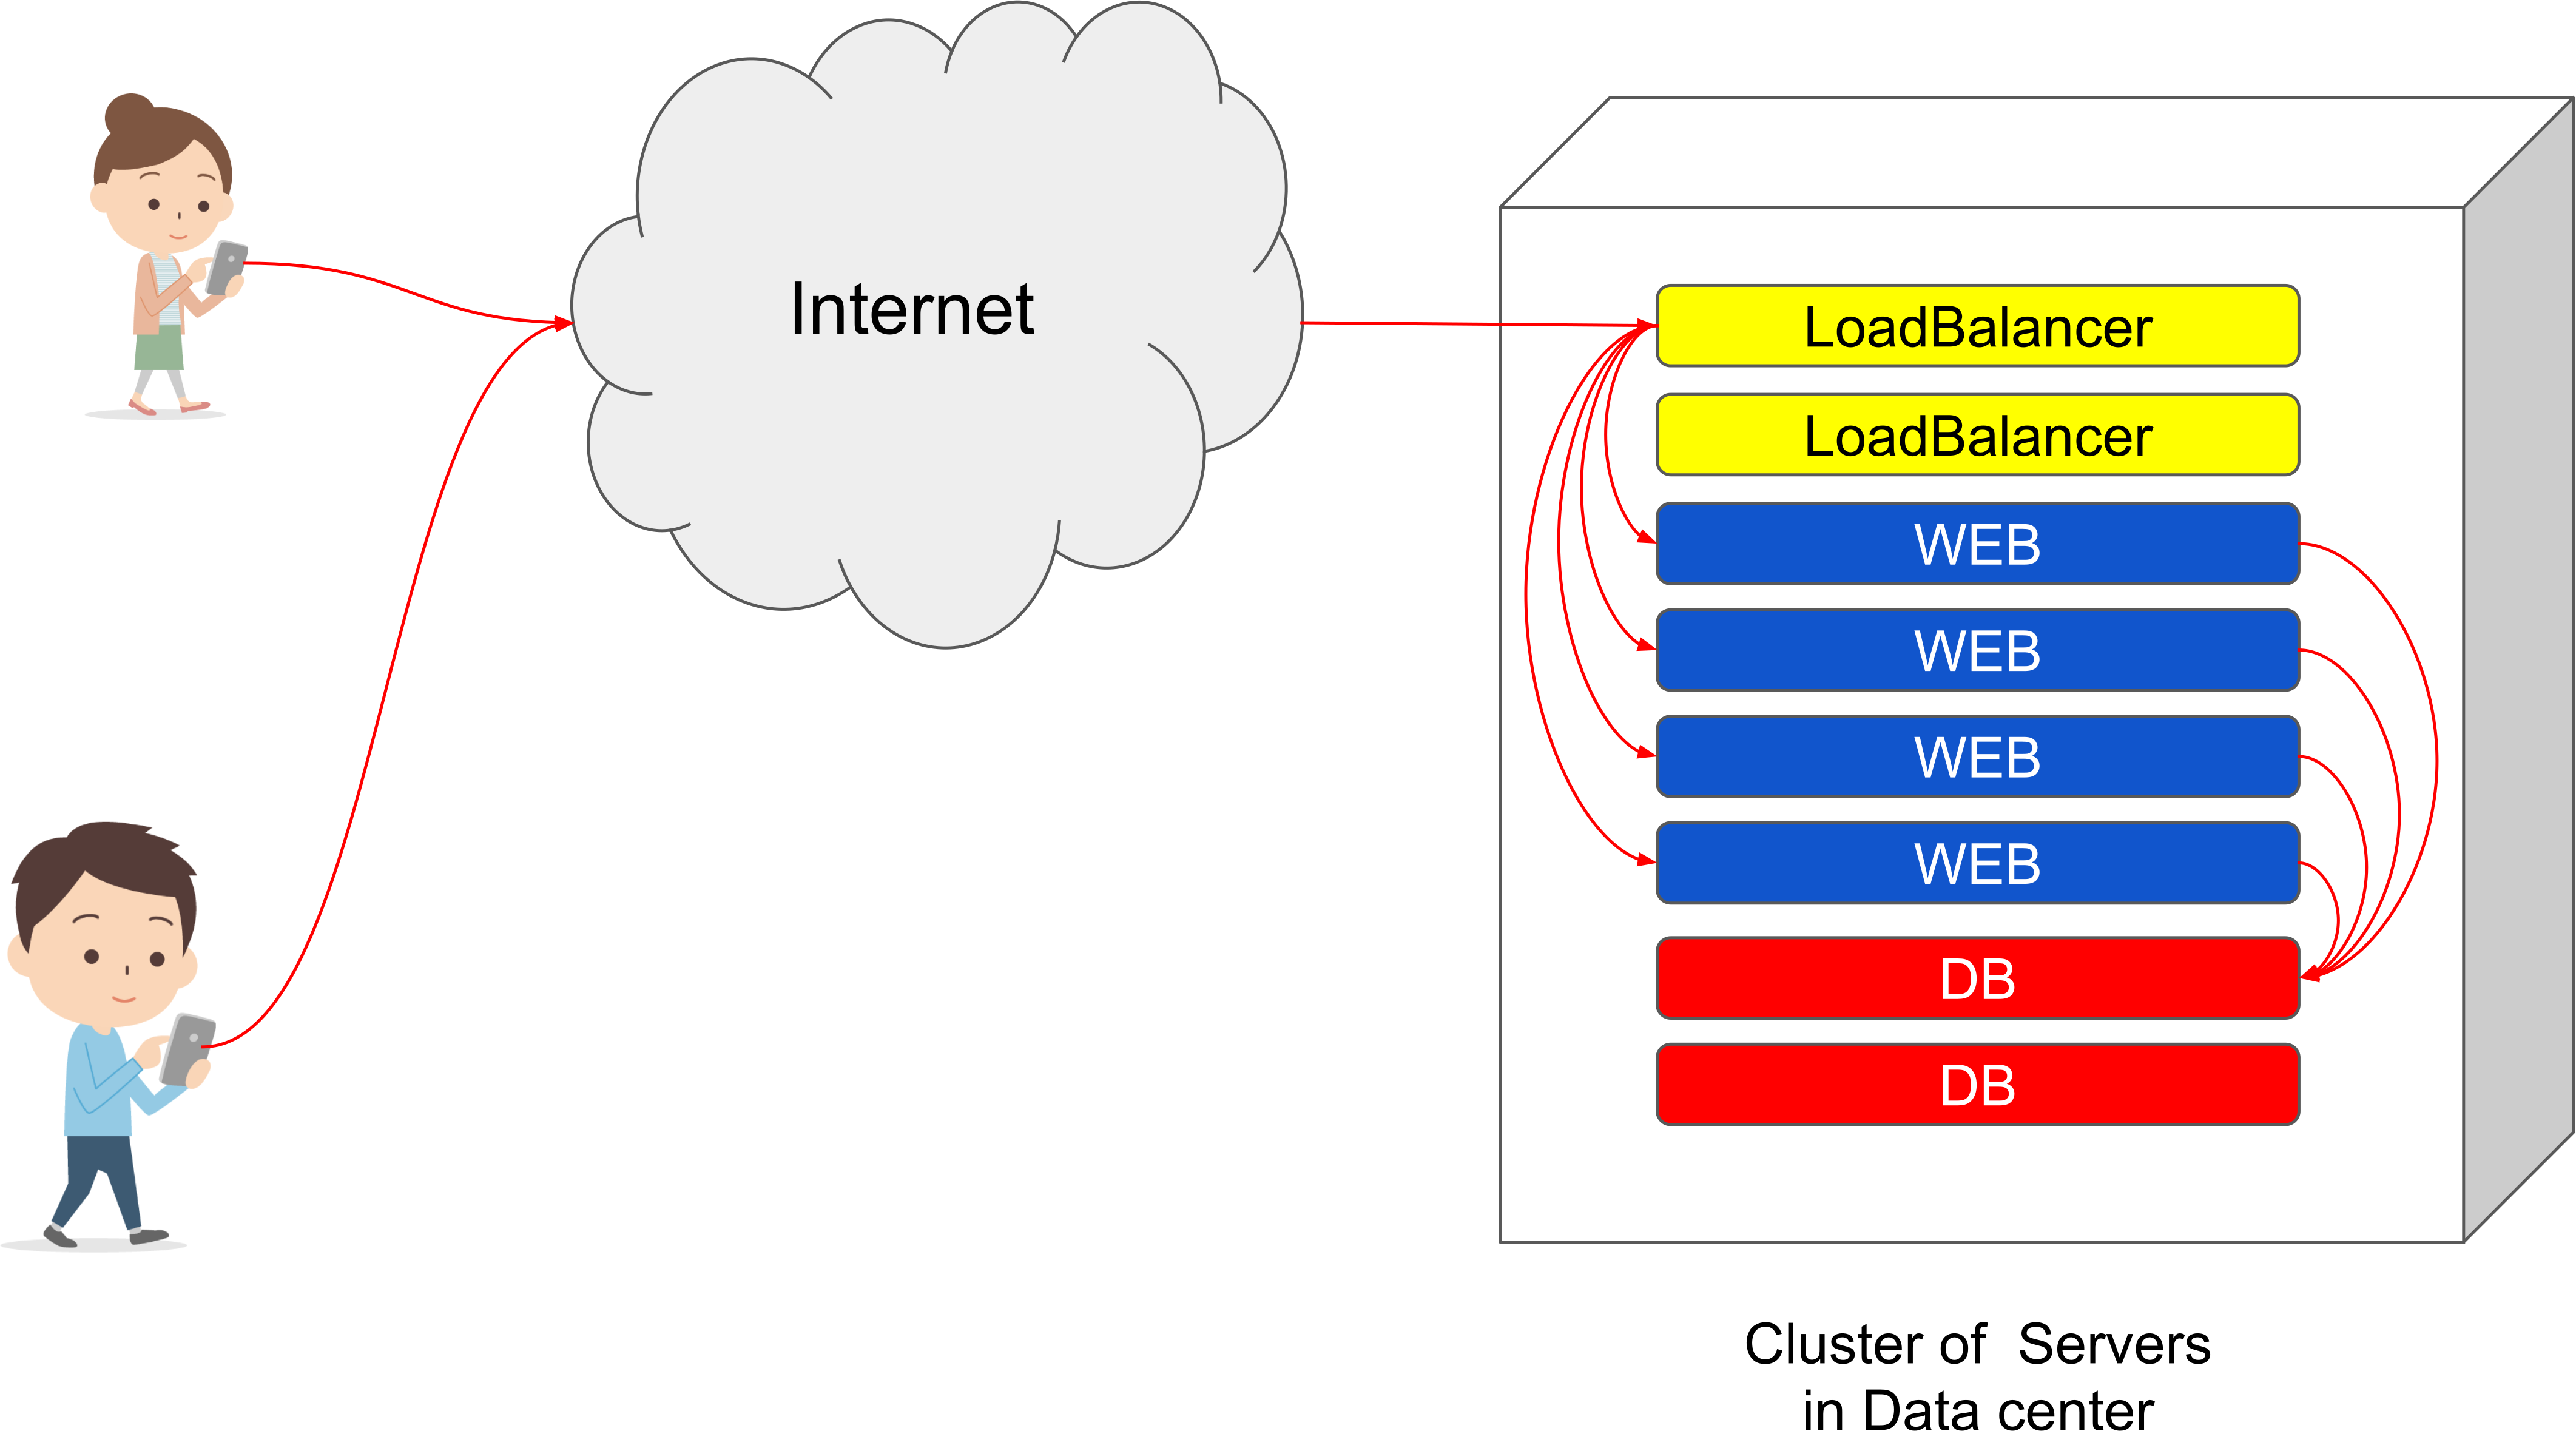
\includegraphics[width=0.8\columnwidth]{Figs/web_cluster.png}
\end{center}
\caption{
An example of web cluster.
}
\label{fig:web_cluster}
\end{figure}

In this example, there are two load balancers, four web servers and two Database(DB) servers that work together to respond to requests from clients.
The load balancers distribute requests from clients to multiple web servers. 
Then the web servers form the response using the data retrieved from the database servers, and send it back to the client.
Sometimes the web servers may store and update important data into the database servers.

\subsection{On-premise datacenter}

Web application providers often purchase these servers and locate them in server housing facilities called data centers.
In this type of infrastructure, the web application providers typically need to sign a contract with data center company for server housing racks, buy servers and install them in their rented racks by themselves.
Since the servers are located in the users own facilities or rented facilities, and the users are responsible for managing those servers, this type of infrastructure is often called on-premise infrastructure so as to contrast Cloud Computing infrastructure.
Preparing data centers, installing the servers and configuring software stacks for their services often require considerable amount of time and money.
If they want to expand their services to different countries or if they want to prepare for natural disasters by preparing an additional web cluster in a different data center, they most likely need about the same amount of time, money and effort required to build their original infrastructures.

\subsection{Cloud computing}

The emergence of Cloud Computing made many things easier for web application providers than before.
Cloud computing utilizes a virtual machine(VM) technology, e.g. KVM, Xen, and VMware.
Cloud computing providers offer VMs to web application providers(users) with pay-per-use billing.

\begin{figure}[h]
\begin{center}
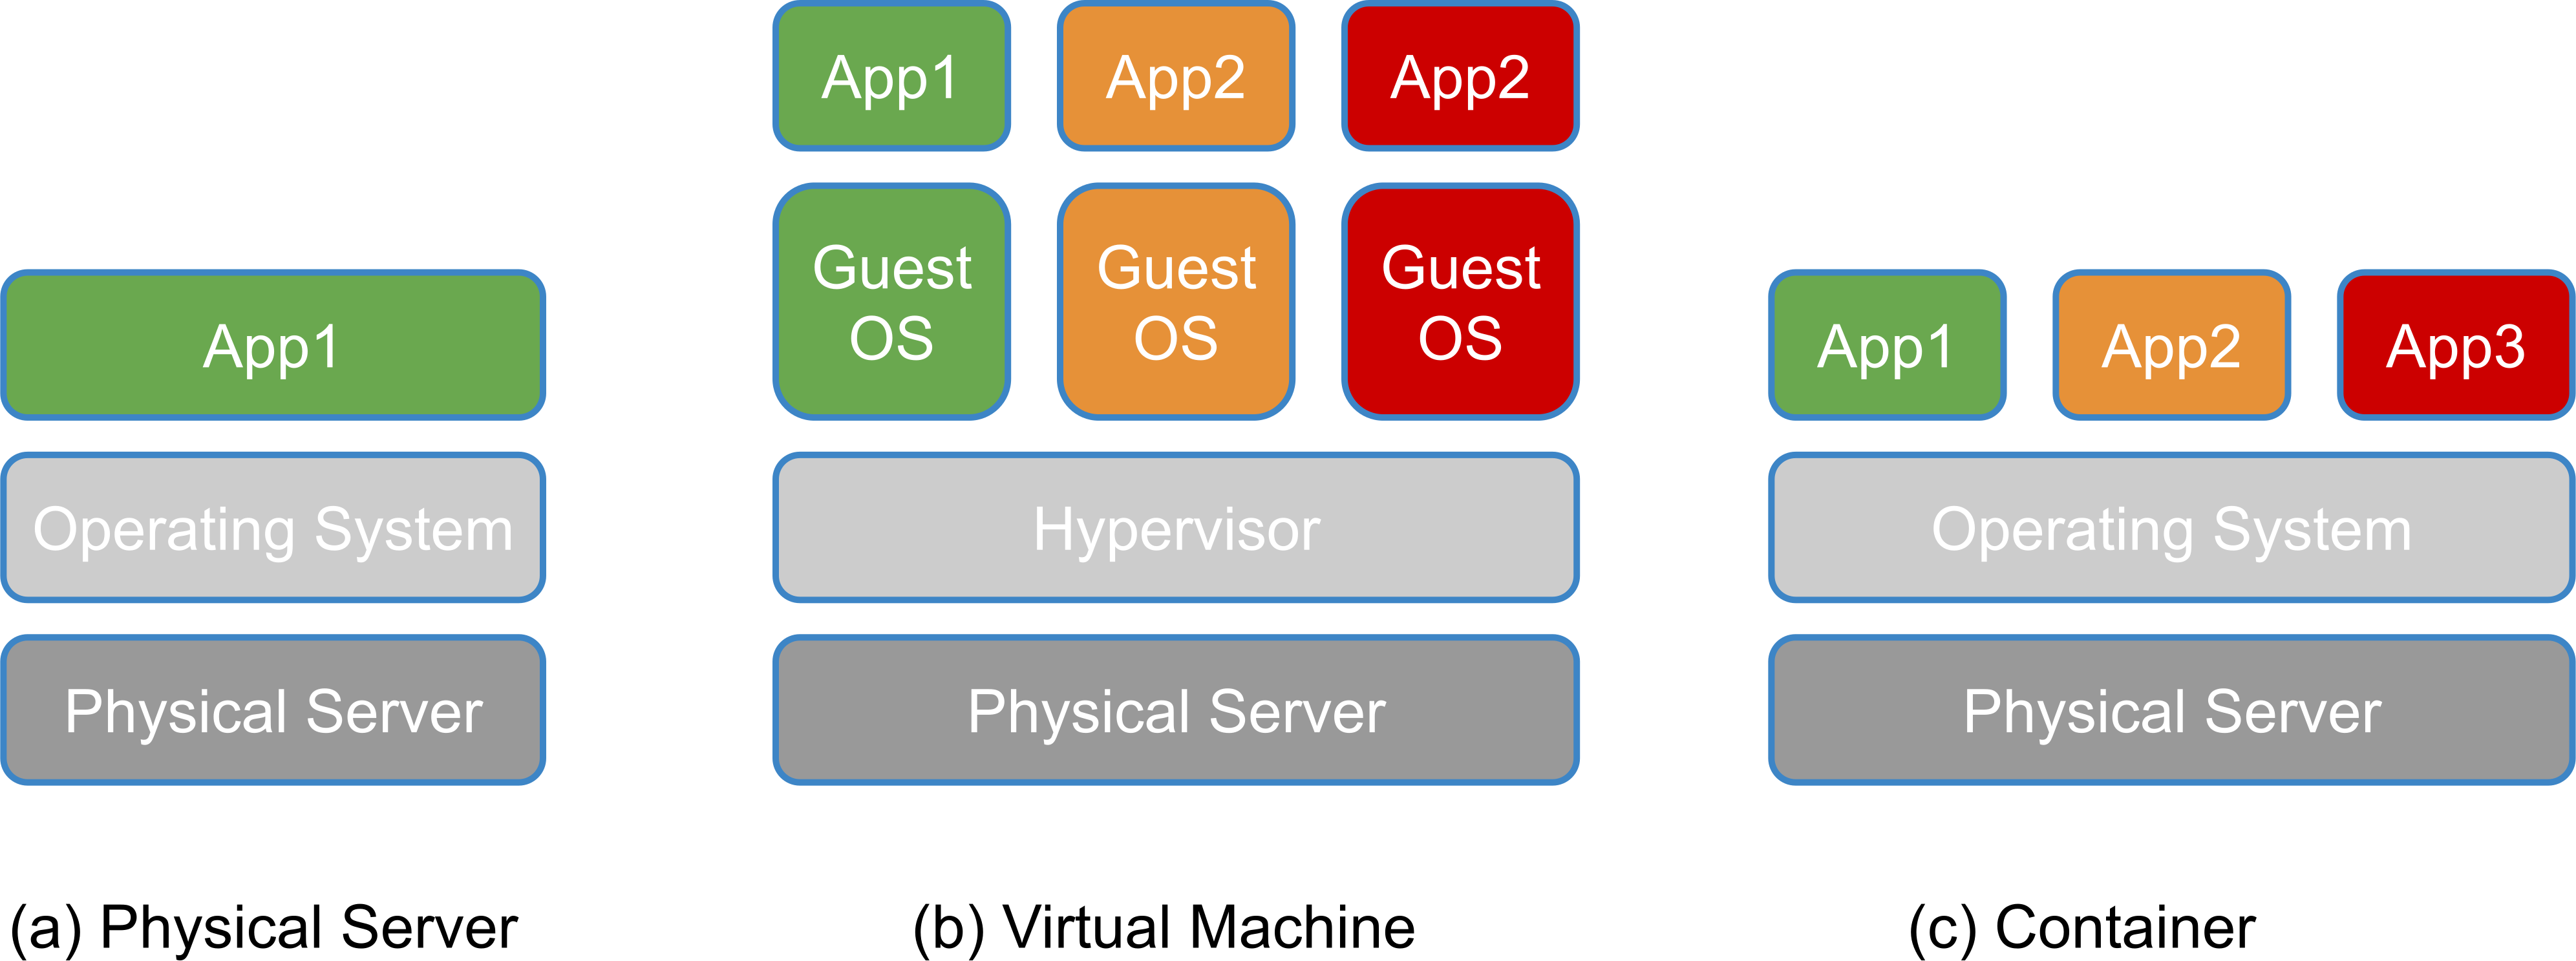
\includegraphics[width=0.8\columnwidth]{Figs/physical_vm_container.png}
\end{center}
\caption{
The difference in physical server usage between (a) Bare Metal servers, (b) Virtual Machine and (c) Container technology.
(a) Bare Metal servers is a word to describe conventional physical servers in contrast to Virtual Machines.
On top of a Bare Metal server, an operating system and application programs are runnig.
(b) Virtual Machine technology utilizes physical server hardware and a hypervisor.
The hypervisor provides generic representations of server hardware, which are called virtual machines.
A full operating system and applications are running on each of the virtual machines.
(c) Container technology separates applications by containing them to their respective namespaces.
Applications can not see each other's filesystems, networks, users and process IDs unless they belong to the same namespace.
Since container technology merely relies on Linux kernel's namespace function and optionally cgroup, a containerized process does not have any additional overhead compared with a process running on a conventional physical server and operating system.
Container technology can be also utilized on top of virtual machines.
}
\label{fig:physical_vm_container}
\end{figure}

Figure~\ref{fig:physical_vm_container} (b) shows an example architecture of VM technology. 
VMs share a single physical server.
A full OS including Linux kernel is running on top of the virtual machine represented by the hypervisor.
Each VM behaves almost as same as a single physical server.
Since VMs are fractions of a single physical server, server resources are utilized with finer granularities.
Users can start their services with a cluster of VMs, which is smaller than a cluster of physical servers, and hence resulting in lower cost.
Cloud providers prepare physical servers and software stacks for VMs before renting it to users.
As a result, users need only to click a few buttons on web browsers, before up-and-running VMs are available for them.
This easiness will bring agility to users when they launch their services.
And since computing resources are offered with per-second pay-per-use billing, users can quickly reduce the cost by stopping excessive VMs, when the demand for computing power decreases.
This was impossible when web application providers purchased physical servers and installed them in a conventional data center.
In short cloud computing brought the users agility, flexibility, and cost-effectiveness.

\subsection{Container technology}

More recently, Linux containers\cite{menage2007adding} have come to draw a significant amount of attention.
Figure~\ref{fig:physical_vm_container} (c) shows an example architecture of container technology. 
Container technology utilizes Linux kernel's namespace feature to separate process execution environments.  
Every process is assigned to a certain namespace, and if two processes belong to different namespaces, they can not see each other's resources. 
Linux kernel implements filesystem, PID, network, user, IPC, and hostname namespaces. 
For example, each filesystem namespace has its own root filesystem, and each network namespace has its own network devices and IP addresses.
Therefore, it is possible to configure processes as if they were running in different Linux systems by assigning them to different namespaces, although they share kernel and hardware.
Whilst VMs needed to run a full OS on top of a hypervisor and hence imposing extra overhead, a process in Linux containers is as light as a single process because it merely belongs to its respective namespace.
%
Several management tools are available for Linux containers, including LXC\ref{}, systemd-nspawn\ref{}, lmctfy\ref{} and Docker\ref{}.
These tools restore file system from image (archive) file, setup network interfaces, launch processes, and assign appropriate namespaces.
Due to the widespread usage of Linux systems, Linux containers can run in most of the cloud infrastructures and on-premise data centers.
Linux containers are reproducible because the process execution environments are archived into tar files.
Whenever one attempts to run a container, the exact same file systems are restored from the archive.
Therefore a process in a container is expected to behave exact same manner, even when totally different data centers or cloud providers are used.
This was not easy when there was no container technology, because there are many flavors of Linux distributions and hence there was a possibility that the program binary and libraries were not identical, whenever one attempted to run a process.
A single update of a library might have broken the expected behavior.
%
Thanks to these benefits, i.e., Linux containers are generally more lightweight, portable and reproducible than virtual machines(VMs), cloud providers are starting to offer services utilizing container technologies.

For these reasons, Linux containers are attractive for web applications as well, and it is expected that web applications consisting of a cluster of containers can be run anywhere regardless of the difference in base infrastructures, i.e. cloud providers or data centers.

\subsection{Container Management System}


Docaker Swarm, Kubernetes, Marathon
Container orchestrator.

Container management system schedule containers

Another aspect of the container management system is interesting. 
It can be viewed as the Operating System for a cluster of servers, where it not only provides scheduling of proccesses but also route the traffic to the right processes.
In this way, a cluster of computers can be used to provide web services with the ease of using a single computer.



migrated easily for a variety of purposes.
For example disaster recovery, cost performance optimizations, meeting legal compliance and shortening the geographical distance to customers are the main concerns for web application providers in e-commerce, gaming, Financial technology(Fintech) and Internet of Things(IoT) field.

The purpose of this research is to enable web application providers to easily deploy their services across the world seamlessly, regardless of cloud providers or data centers they use, by better-utilizing container cluster technology. 
Also, the author aims to realize the future where users can choose whatever infrastructure they like without sacrificing advanced features that are provided only by limited cloud providers.


\subsection{Desireble infrastructure using container}

\begin{itemize}
\item Universal Container management system as a middle ware
\item Global data storage as Google spanner, Conckroach database
\item Global routing, Anycast 
\end{itemize}

The author focus on Load balancer.
Software load balancer that work well with container env.

\begin{itemize}
\item How is the performance?
\item How is that scable?
\end{itemize}



\section{Avoid lock-in problem}

It is desirable if users can migrate their services to multiple of cloud providers or on-premise data centers seamlessly, which spread across the world.
Container cluster management systems facilitate these usages by functioning as middlewares, which hide the differences among cloud providers and on-premise data centers.

Kubernetes\cite{K8s2017}, which is one of the most popular container cluster management systems, enables easy deployment of container clusters.
Kubernetes are initially developed by engineers inside Google, to facilitate container cluster deployment for web applications.
Kubernetes allows users to deploy a cluster of containers each of which depends on each other, with the ease of launching a single application program.
It also allows users to increase or decrease the number of containers dynamically depending on the amount of traffic that they have to respond.

Since Kubernetes is expected to hide the differences in the base environments, it is expected that users can easily deploy a web application on different cloud providers or on on-premise data centers, without adjusting the container cluster configurations to the new environment. 
This allows a user to easily migrate a web application consisting of a container cluster even to the other side of the world.
A typical web application migration scenario is; 
a user starts the container cluster in the new location, route the traffic there, then stop the old container cluster at his or her convenience.

However, this scenario only works when the user migrates a container cluster among major cloud providers including Google Cloud Platform (GCP), Amazon Web Applications (AWS), and Microsoft Azure.
This is because Kubernetes fails to completely hide differences in base environments.
Kubernetes does not provide generic ways to route the traffic from the internet into container cluster running in the Kubernetes and expects the base infrastructure automatically route traffic to nodes that might host container.
In other words, Kubernetes is heavily dependent on cloud load balancers, which is external load balancers that are set up on the fly by cloud providers through their application protocol interfaces (APIs).
Once the traffic reaches the nodes, Kubernetes handles it nicely, but this is a problem since not every cloud provider or on-premise data center has load balancers that can be set up through API and utilized by Kubernetes.
Other container cluster management systems, e.g. Docker swarm, etc, also lack a generic way to route the traffic into the container cluster.
Therefore this is one of the generic problems that current container cluster architectures possess.

Load balancers are often used to distribute high volume traffic from the Internet to thousands of web servers.
They are implemented as dedicated hardware or software on commodity hardware.
Major cloud providers have developed software load balancers\cite{eisenbud2016maglev,patel2013ananta} as a part of their infrastructures.
They claim that their load balancers have a high-performance level and scalability.
Those software load balancers have APIs through which an outside program can set up and control the behavior of the load balancers.
Once cloud load balancers are set up automatically and distribute incoming traffic to every server that hosts containers,
the traffic is then distributed again to destination containers using the iptables destination network address translation(DNAT)\cite{MartinA.Brown2017,Marmol2015} rules in a round-robin manner.

In the case of on-premise data centers, there are variety of proprietary hardware load balancers.
It is very likely that most of the load balancers are left unsupported by Kubernetes, even if some of the load balancers may have APIs through which a container management system can set up and control the behavior.
In these cases, the user needs to manually configure the static route for inbound traffic in an ad-hoc manner.
Since the Kubernetes fails to provide a uniform environment from a container cluster viewpoint, migrating container clusters among the different environments will always require daunting tasks.
One of the aims of this study is to seek a generic way to route the traffic into container clusters automatically, by providing a software load balancer that works well with the container management systems, and thereby to facilitate web application migrations.

\section{Contribution}

In order to achieve these aims, the author proposes a portable and scalable software load balancer that can be used in any environment including cloud providers and in on-premise data centers.
By using such a load balancer, users do not need to manually adjust their services to the base infrastructures.
As a proof of concept the author implements the proposed software load balancer that works well with with Kubernetes using following technologies;
1) To make the load balancer usable in any environment, Linux kernel's Internet Protocol Virtual Server (ipvs)\cite{Zhang2000} is containerized using Docker\cite{merkel2014docker}. 
2) To make the load balancer redundant and scalable, the author makes it capable of updating the routing table of upstream router with Equal Cost Multi-Path(ECMP) routes\cite{al2008scalable} using a standard protocol, Border Gateway Protocol(BGP).
3) The author also extends the research into implementing the novel load balancer using eXpress Data Plane(XDP) technology\cite{bertin2017xdp} to enhance the performance level to meet the need for 10Gbps network speed.

Contributions of this paper are as follows:
Although there have been studies regarding redundant software load balancers especially from the major cloud providers\cite{eisenbud2016maglev,patel2013ananta}, their load balancers are only usable within their respective cloud infrastructures.
Therefore in order to facilitate container cluster migrations, a software load balancer architecture with redundancy and scalability that is common to any base infrastructure has been needed.
This paper aims to provide such a load balancer architecture and evaluate a proof-of-concept system that is built using Open Source Software(OSS) technologies.
The understanding obtained from a detailed analysis of the evaluation also helps both the research community and the web application industry, because there does not exist enough of them.
Moreover, since proposed load balancer architecture uses nothing but existing OSSs and standard Linux boxes, users can build a cluster of redundant load balancers in their environment.

The outcome of this study will benefit users who want to deploy their web applications on any cloud provider where no scalable load balancer is provided, to achieve high scalability.
Moreover, the result of our study will potentially benefit users who want to use a group of different cloud providers and on-premise data centers across the globe seamlessly.
In other words, users will become being able to deploy a complex web application on aggregated computing resources on the earth, as if they were starting a single process on a single computer.

\section{Outline}

The rest of the paper is organized as follows.
Chapter \ref{chapter:background} provides the background information and related works.
Chapter \ref{chapter:architecture} provides the problems of existing load balancers and proposes suitable architectures.
Chapter \ref{chapter:implemetation} presents implementation of the proposed load balancer architecture in detail.
Chapter \ref{chapter:portablelb} discusses portability and performance levels of the proposed load balancer in 1 Gbps network environment.
Chapter \ref{chapter:redundancy} discusses the redundancy and scalability of the proposed load balancers.
Chapter \ref{chapter:performance} present the performance levels of the proposed load balancer in 10 Gbps network environment and discuss the method to improve the performance of a software load balancer.
Chapter \ref{chapter:futurework} discusses the limitation and the future work of this study,
which is followed by a conclusion of this work in Chapter \ref{Conclusions}.







\chapter{Background}\label{chapter:Background}
\subsection{Flannel}

We used flannel to build the Kubernetes cluster used in our experiment.
Flannel has three types of backend, {\it i.e.}, operating modes, named host-gw, vxlan, and udp\cite{CoreOSFlannelBackend}.

In the host-gw mode, the flanneld installed on a node simply configures the routing table 
based on the IP address assignment information of the overlay network, which is stored in the etcd. 
When a {\em pod} on a node sends out an IP packet to {\em pods} on the different node, 
the former node consults the routing table and learn that the IP packet should be sent out to the latter.
Then, the former node forms Ethernet frames containing the destination MAC address of the latter node 
without changing the IP header, and send them out.

In the case of the vxlan mode, flanneld creates the Linux kernel's vxlan device, flannel.1. 
Flanneld will also configures the routing table appropriately based on the information stored in the etcd.
When {\em pods} on different nodes need to communicate, the packet is routed to flannel.1.
The vxlan functionality of the Linux kernel identify the MAC address of flannel.1 device on the destination node,
then form an Ethernet frame toward the MAC address.
The vxlan then encapsulates the Ethernet frame in a UDP/IP packet with a vxlan header, after which the IP packet is eventually sent out.

In the case of udp mode, flanneld creates the tun device, flannel0, and configures the routing table.
The flannel0 device is connected to the flanneld daemon itself.
An IP packet routed to flannel0 is encapsulated by flanneld, and eventually sent out 
to the appropriate node. 
The encapsulation is done for IP packets.

Figure~\ref{fig:flannel-packet-diagram} shows the schematic diagrams of frame formats for three backends modes of the flannel overlay network. 
The MTU sizes in the backends, assuming the MTU size without encapsulation is 1500 bytes, are also presented.
Since packets are not encapsulated in the host-gw mode, the MTU size remains 1500 bytes.
An additional 50 bytes of header is used in the vxlan mode, thereby resulting in an MTU size of 1450 bytes.
In the case of the udp mode, only 28 bytes of header are used for encapsulation, which results in an MTU size of 1472 bytes.

\begin{figure}
  \centering
  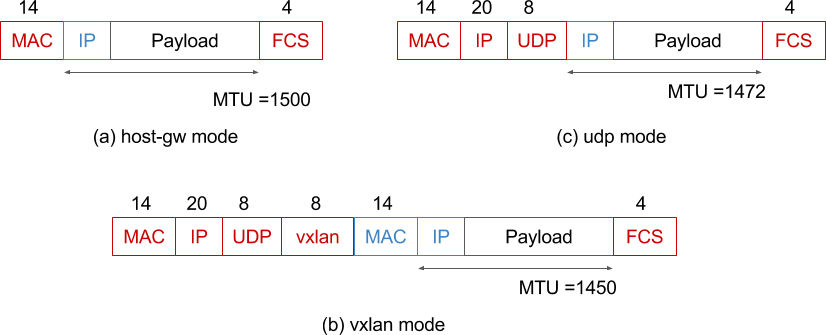
\includegraphics[width=0.8\columnwidth]{Figs/flannel-packet-diagram}
  \caption{frame diagram}
  \label{fig:flannel-packet-diagram}
\end{figure}

Performance of the load balancers can be influenced by the overhead of encapsulation. 
Thus, the host-gw mode, where there is no overhead due to encapsulation, 
results in the best performance levels as shown in Section~\ref{Result and Discussion}.
However, the host-gw mode has a significant drawback that prohibit it to work correctly in cloud platforms. 
Since the host-gw mode simply sends out a packet without encapsulation, if there is a cloud gateway between nodes, 
the gateway cannot identify the proper destination, thus drop the packet.

\begin{table}
  \centering
  \begin{tabular}{lccc}
    \toprule
    mode & On-premise & GCP & AWS \\
    \midrule
    host-gw & OK & NG & NG \\
    vxlan & OK & OK & OK \\
    udp & OK & OK & OK \\
    \bottomrule
\end{tabular}

  \caption{Viable flannel backend modes. In cloud environment tunnelig using vxlan or udp is needed.}
  \label{tab:Viable flannel backends}
\end{table}

We conducted an investigation to determine which of the flannel backend mode would be usable on AWS, GCP, and on-premise data centers.
The results are summarized in Table~\ref{tab:Viable flannel backends}. 
In the case of GCP, an IP address of {\tt /32} is assigned to every VM host and 
every communication between VMs goes through GCP's gateway.
As for AWS, the VMs within the same subnet communicate directly, while the VMs in different subnets communicate via the AWS's gateway.
Since the  gateways do not have knowledge of the flannel overlay network, they drop the packets; thereby, 
they prohibit the use of the flannel host-gw mode in those cloud providers.  

In our experiment, we compared the performance of load balancers when different flannel backend modes were used. 

\paragraph{\bf host-gw}
\paragraph{\bf vxlan}
\paragraph{\bf udp}

\subsection{Calico}
\paragraph{\bf no-tunnel}
\paragraph{\bf ipip}

\section{Multicore Packet Proccessing}

Recently, the performance of CPUs are improved significantly due to the development of multi-core CPUs.
One of the top of the line server processors from Intel now includes up to 28 cores in a single CPU.
In order to enjoy the benefits of multi-core CPUs in communication performance, 
it is necessary to distribute the handling of interrupts from the NIC and the IP protocol processing to the available physical cores.

\subsection{rss}

Receive Side Scaling (RSS)\cite{TomHerbert} is a technology 
to distribute handling of the interrupt from NIC queues to multiple CPU cores.
Subsequently, Receive Packet Steering (RPS)\cite{TomHerbert} distributes the IP protocol processing 
to multiple CPU cores by issuing inter core software interrupts.

Since load balancer performance levels could be affected by these technologies,
we conducted an experiment to determine how load balancer performance level change depending on the RSS and RPS settings.
The following shows how RSS and RPS are enabled and disabled in our experiment. 
The NIC used in our experiment is Broadcom BCM5720, which has four rx-queues and one tx-queue.
Figure~\ref{fig:rx-queue} shows the interrupt request (IRQ) number assignments to those NIC queues.

\begin{figure}
\centering
\begin{minipage}{0.5\columnwidth}
\begin{verbatim}
81: eth0-tx-0
82: eth0-rx-1
83: eth0-rx-2
84: eth0-rx-3
85: eth0-rx-4
# obtained from /proc/interrupts 
\end{verbatim}
\end{minipage}
\caption{RX/TX queues of the hardware}
\label{fig:rx-queue}
\end{figure}

When packets arrive, they are distributed to these rx-queues depending on the flow each packet belongs to.
Each receive queue has a separate IRQ associated with it. The NIC triggers
this to notify a CPU when new packets arrive on the given queue.
Then, the notified CPU handles the interrupt, and performs the protocol processing. 
According to the \cite{TomHerbert}, the CPU cores allowed to be notified is controlled by setting 
a hexadecimal value corresponding to the bit maps indicating the allowed CPU cores in \enquote{/proc/irq/\$irq\_number /smp\_affinity}.
%
For example, in order to route the interrupt for eth0-rx-1 to CPU0, 
we should set \enquote{/proc/irq/82/smp\_affinity} 
to binary number {\tt 0001}, which is 1 in hexadecimal value.
Further, in order to route the interrupt for eth0-rx-2 to CPU1, we 
should set \enquote{/proc/irq/83/smp\_affinity} 
to binary number {\tt 0010}, which is 2 in hexadecimal value.

We refer the setting to distribute interrupts from four rx-queues to CPU0, CPU1, CPU2 and CPU3 as {\tt RSS = on}. 
It is configured as the following setting: 

\begin{center}
\begin{minipage}{0.6\columnwidth}
\begin{Verbatim}[commandchars=\\\{\}]

\underline{\textbf{RSS=on}}
echo 1 > /proc/irq/82/smp_affinity
echo 2 > /proc/irq/83/smp_affinity
echo 4 > /proc/irq/84/smp_affinity
echo 8 > /proc/irq/85/smp_affinity

\end{Verbatim}
\end{minipage}
\end{center}

On the other hand, {\tt RSS = off} means that an interrupt from any rx-queue is routed to CPU0. 
It is configured as the following setting:

\begin{center}
\begin{minipage}{0.6\columnwidth}
\begin{Verbatim}[commandchars=\\\{\}]

\underline{\textbf{RSS=off}}
echo 1 > /proc/irq/82/smp_affinity
echo 1 > /proc/irq/83/smp_affinity
echo 1 > /proc/irq/84/smp_affinity
echo 1 > /proc/irq/85/smp_affinity

\end{Verbatim}
\end{minipage}
\end{center}

%In this case, interrupt from any of rx-queue is routed to CPU0.
\subsection{rps}

The RPS distributes IP protocol processing by placing the packet
on the desired CPU's backlog queue and wakes up the CPU using inter-processor interrupts.
We have used the following settings to enable the RPS:

\begin{center}
\begin{minipage}{0.8\columnwidth}
\begin{Verbatim}[commandchars=\\\{\}]

\underline{\textbf{RPS=on}}
echo fefe > /sys/class/net/eth0/queues/rx-0/RPS_cpus
echo fefe > /sys/class/net/eth0/queues/rx-1/RPS_cpus
echo fefe > /sys/class/net/eth0/queues/rx-2/RPS_cpus
echo fefe > /sys/class/net/eth0/queues/rx-3/RPS_cpus

\end{Verbatim}
\end{minipage}
\end{center}

Since the hexadecimal value \enquote{fefe} represented as \enquote{1111 1110 1111 1110} in binary, 
this setting will allow distributing protocol processing to all of the CPUs, except for CPU0 and CPU8.
In this paper, we will refer this setting as {\tt RPS = on}.
%
On the other hand, {\tt RPS = off} means that no CPU is allowed for RPS. 
Here, the IP protocol processing is performed on the CPUs the initial hardware interrupt is received.
It is configured as the following settings:

\begin{center}
\begin{minipage}{0.8\columnwidth}
\begin{Verbatim}[commandchars=\\\{\}]

\underline{\textbf{RPS=off}}
echo 0 > /sys/class/net/eth0/queues/rx-0/RPS_cpus
echo 0 > /sys/class/net/eth0/queues/rx-1/RPS_cpus
echo 0 > /sys/class/net/eth0/queues/rx-2/RPS_cpus
echo 0 > /sys/class/net/eth0/queues/rx-3/RPS_cpus

\end{Verbatim}
\end{minipage}
\end{center}

The RPS is especially effective when the NIC does not have multiple receive queues or when the number of queues is 
much smaller than the number of CPU cores. 
That was the case of our experiment, where we had a NIC with only four rx-queues, 
while there was a CPU with eight physical cores.

\subsection{rps}
\subsection{Others}
\paragraph{rfs}
\paragraph{xps}
\paragraph{xfs}

\section{Other parameters}
\subsection{tcp congestion mode}

\section{Cloud Load Balancers}
\subsection{Maglev}
\subsection{Ananta}
\subsection{GCP Load Balancer}
GCP experimental data.


\chapter{Architecture and Implementation}\label{chapter:Architecture and Implementation}
One of the most important problems of existing container orchestrators is that none of them has full support for automatically setting up routes for ingress traffic in a redundant and scalable manner.
In order to solve this problem, the author proposes a cluster of software load balancer in containers, which is deployed as a part of the web application clusters.
Key features required for such load balancers are;
1) to implement a mechanism where the routing table of the upstream router is updated automatically so that the router can forward ingress traffic to running load balances.
2) to implement software load balancer in a container that is runnable in any environment while having the feature to instantly update load balancing tables so that it can forward the packets to running web application containers.

This chapter provides a discussion of such load balancer architecture.
First, the author discusses problems of conventions architecture in Section~\ref{Problem of Conventional Architecture}.
Then the author proposes a portable software load balancer in a container in Section~\ref{Load balancer in container}, and discusses redundancy architecture using ECMP in Section~\ref{Redundancy with ECMP}.
%
The author also presents an implementation of the proof of the concept system for the proposed load balancer architecture in detail.
The first overall architecture is explained in Section~\ref{sec:poc}.
Then ipvs containerization is explained in detail in Section~\ref{sec:ipvs}.
Finally, the implementation of BGP software container is explained in Section~\ref{sec:bgp}.

\section{Architecture}

In this section the author discusses the architecture of a portable load balancer for container clusters.

\subsection{Problem of Conventional Architecture}\label{Problem of Conventional Architecture}

\begin{figure}[tb]

  \begin{subfigure}[t]{\columnwidth}
    \centering
    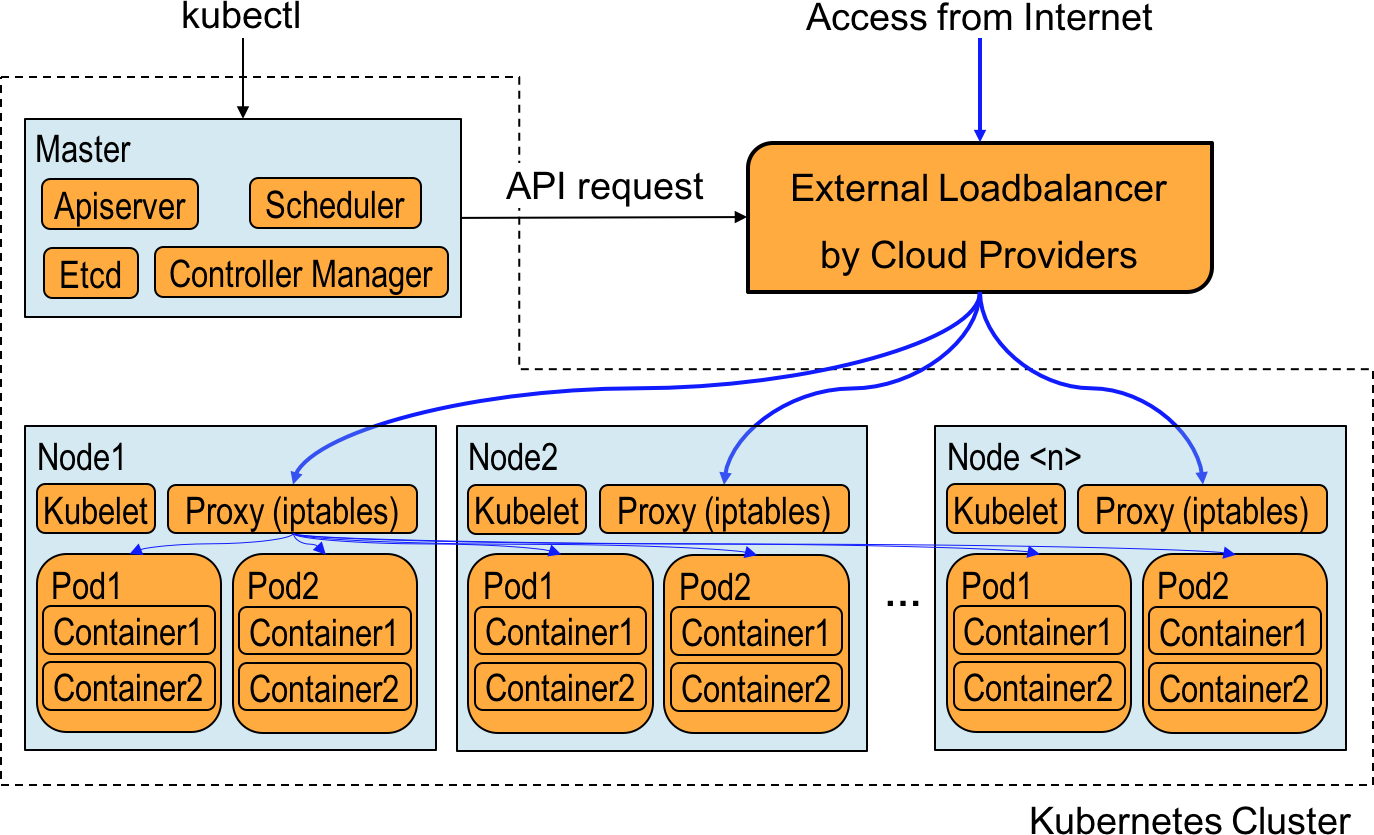
\includegraphics[width=0.8\columnwidth]{Figs/K8sConventional}
    \caption{Kubernetes in cloud infrastructures}
    \label{fig:K8sConventional}
  \end{subfigure}

  \par\bigskip
  \par\bigskip

  \begin{subfigure}[t]{\columnwidth}
    \centering
    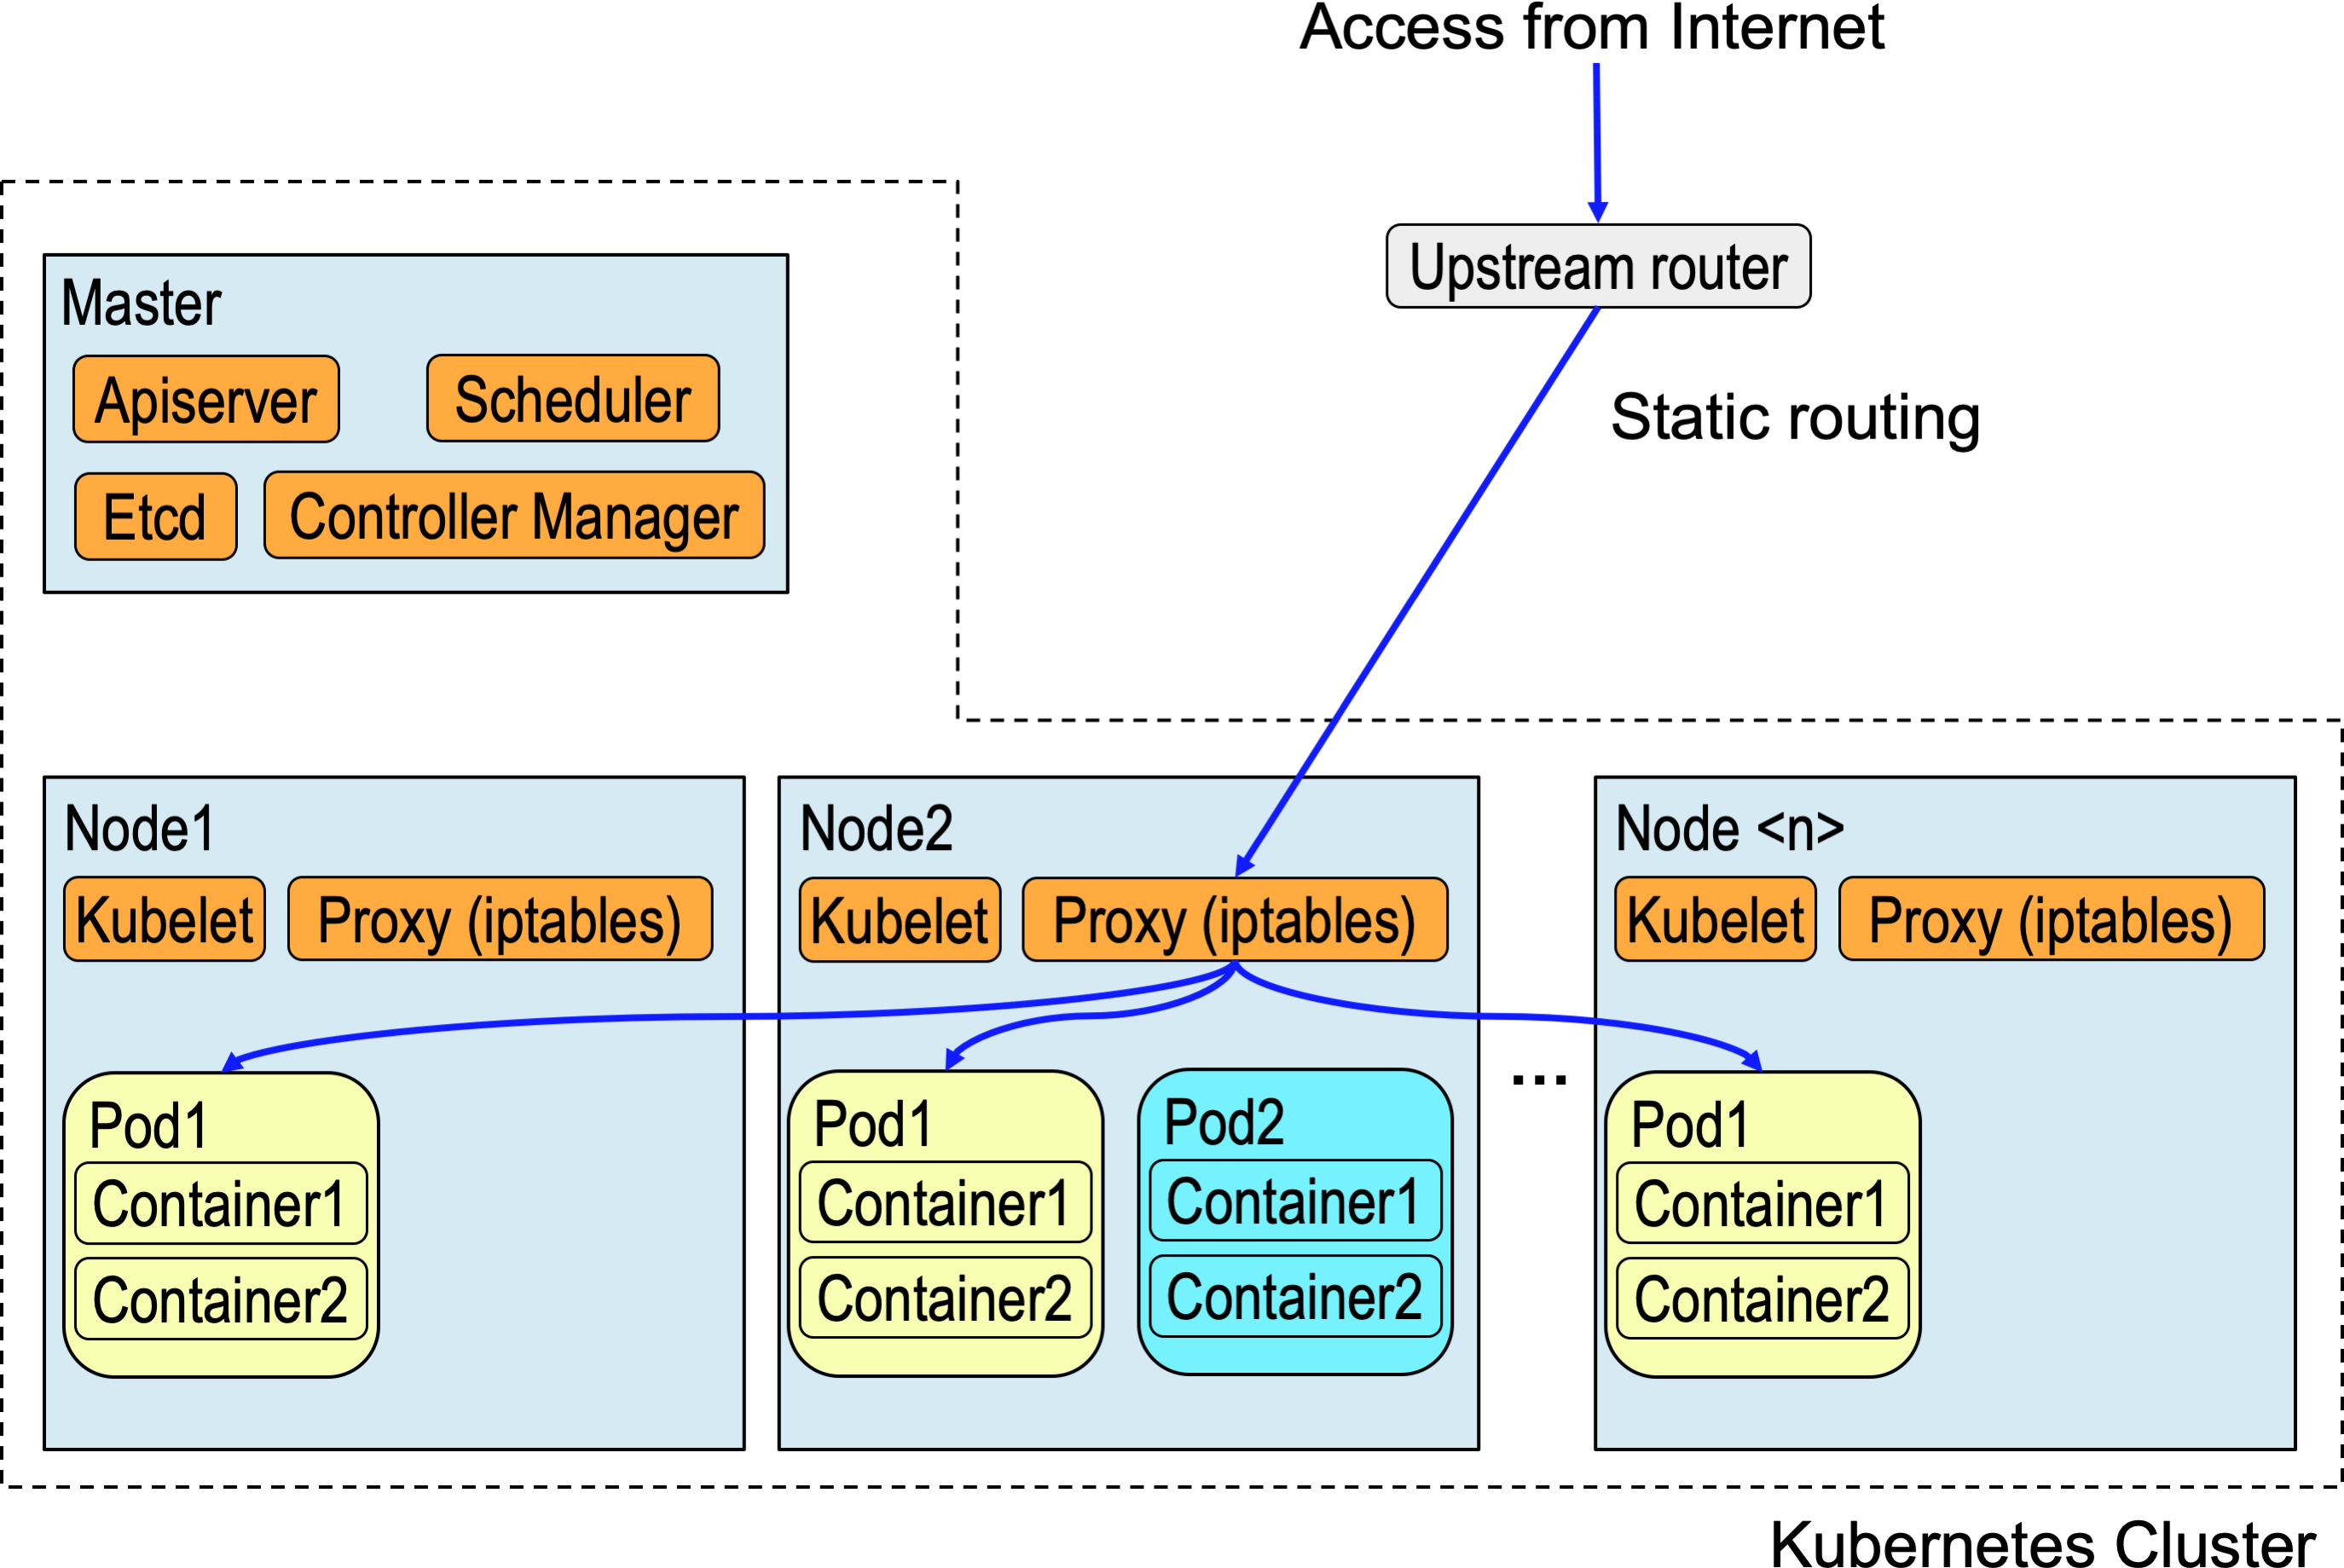
\includegraphics[width=0.8\columnwidth]{Figs/K8sConventional_bm}
    \caption{Kubernetes in on-premise data centers}
    \label{fig:K8sConventional_bm}
  \end{subfigure}

   \centering

  \begin{minipage}{1.0\columnwidth}
    \caption[Conventional architecture of Kubernetes clusters]
            {Conventional architecture of Kubernetes clusters in cloud infrastructure and on-premise data center.
%\small
(a) In supported infrastructures, e.g., major cloud providers, Kubernetes automatically set up the routes for ingress traffic with the help of the external load balancer.
The load balancer distributes ingress traffic to all of the existing nodes.
(b) In unsupported infrastructures, e.g., on-premise data centers, web application providers have to manually set up a route to one of the nodes.
Packets that reached any of the nodes will be distributed to appropriate pods by the iptables DNAT based internal load balancer.
            }
  \end{minipage}

\end{figure}

The problem of Kubernetes is its partial support for the ingress traffic routing.
Figure~\ref{fig:K8sConventional} shows an exemplified Kubernetes cluster.
When a service is created, the master schedules where to run {\em pods}, and kubelets on the nodes launch them accordingly.
At the same time, the master sends out requests to cloud provider's API endpoints, asking them to set up external cloud load balancers that distribute ingress traffic to every node in the Kubernetes cluster.
The proxy daemon on the nodes also setup iptables DNAT\cite{MartinA.Brown2017} rules. 
The Ingress traffic will then be evenly distributed by the cloud load balancer to all the existing nodes, 
after which it will be distributed again by the DNAT rules on the nodes to the designated {\em pods}. 
The returning packets follows the exact same route as the incoming ones.

This architecture has the followings problems: 
1) There must exist cloud load balancers whose APIs are supported by the Kubernetes daemons.
There are numerous load balancers which is not supported by the Kubernetes.
These include the bare metal load balancers for on-premise data centers.
2) Distributing the traffic twice, first on the external load balancers and second on each node, complicates the administration of packet routing. 
Imagine a situation in which the DNAT table on one of the nodes malfunctions.
In such a case, only occasional timeouts would be observed, and hence it would be very difficult to find out which node is malfunctioning.   
3) The ingress traffic is distributed to all the existing nodes in the Kubernetes cluster. 
Suppose there are 1,000 nodes and one of web applications only uses 10 nodes, it seems inefficient and rather complicated to distribute the ingress traffic to all the 1,000 nodes.

Regarding the first problem, if there is no load balancer that is supported by Kubernetes, users must manually set up the static route on the upstream router, every time they launch the web application clusters, as is shown in Figure~\ref{fig:K8sConventional_bm}.
The traffic will be routed to a node and then distributed by the DNAT rules on the node to the designated {\em pods}.
In cases where the upstream router is administered by a data center company, users must always negotiate with them about adding a route to their new application cluster.
This approach significantly lacks simplicity, and degrades the portability of container clusters.
Furthermore, a static route usually lacks redundancy and scalability.

In short, while Kubernetes is effective in major cloud providers, it fails to provide portability for container clusters in environments where there is no supported load balancer. 
And the routes incoming traffic follow are very complex and inefficient.
In order to address these problems, the author proposes a containerized software load balancer 
that is deployable in any environment even if there are no external load balancers.

\FloatBarrier

\subsection{Load balancer in container}\label{Load balancer in container}

The author proposes a load balancer architecture, where a cluster of load balancer containers is deployed as a part of web application cluster.
Figure~\ref{fig:K8sProposed} shows the proposed load balancer architecture for Kubernetes,
which has the following characteristics;
1) A cluster of load balancer containers is deployed as a part of web application cluster.
2) Each load balancer itself is run as a {\em pod} by Kubernetes.
3) Load balancing rules are dynamically updated based on the information about running {\em pods}, which is periodically populated by communicating with apiserver on the master.
4) There exist multiple load balancers for redundancy and scalability.
5) The routing table in the upstream router is updated dynamically using standard network protocol, BGP.

\begin{figure}[h]
  \begin{center}
  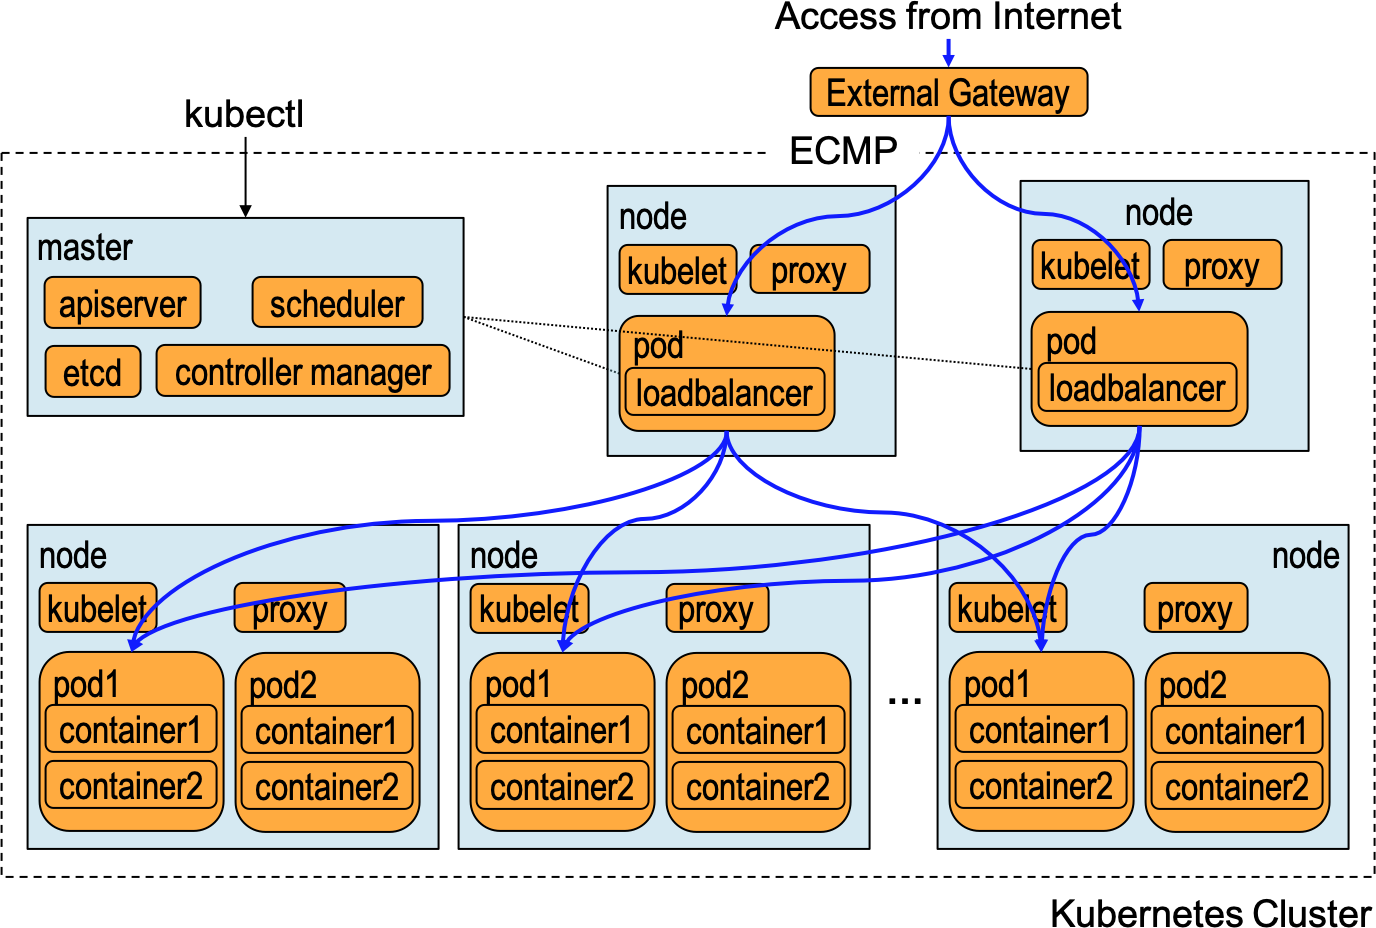
\includegraphics[width=0.8\columnwidth]{Figs/K8sProposed}
  \caption{Kubernetes cluster with proposed load balancer.}
  \label{fig:K8sProposed}
  \begin{minipage}{0.9\columnwidth}
  A cluster of load balancer containers is deployed as a part of web application cluster.
  Each load balancer itself is run as a {\em pod} in the Kubernetes cluster. 
  Load balancing rules are dynamically updated based on the information about running {\em pods}.
  There exist multiple load balancers for redundancy and scalability.
  The routing table in the upstream router is updated dynamically using standard network protocol, BGP.
  \end{minipage}
  \end{center}
\end{figure}

The proposed load balancer can resolve the conventional architecture problems.
Since the load balancer itself is containerized, the load balancer can run in any environment including on-premise data centers,
even without external load balancers that is supported by Kubernetes.
The incoming traffic is directly distributed to designated {\em pods} by the load balancer.
It makes the administration, e.g. finding malfunctions, easier.
Since the proposed load balancers are deployed as a part of web application cluster and the routes to the load balancers are set up automatically through BGP, users do not need to manually set up a static route to a load balancer.

Furthermore, the proposed load balancer has other benefits.
Since a software load balancer in a container can run on any Linux system, it can share the server pool with web containers.
Users can utilize existing servers rather than buying dedicated hardware.

Because a cluster of load balancer containers is controlled by Kubernetes, it becomes redundant and scalable.
Kubernetes always tries to maintain the number of load balancer containers as same as the number specified by the user.
If a single container fails, Kubernetes schedule and launch another one on a different node, which provides the resilience to failures.
When there is a huge spike in the traffic, user can quickly scale the size of the cluster depending on the demand.

The routes to the load balancers are automatically updated through the standard protocol, BGP.
Therefore users do not need to manually add the route every time new load balancer container is launched, as is the case in the conventional architecture.

\FloatBarrier

\subsection{Redundancy with ECMP}\label{Redundancy with ECMP}

\begin{figure}[tb]
  \centering
  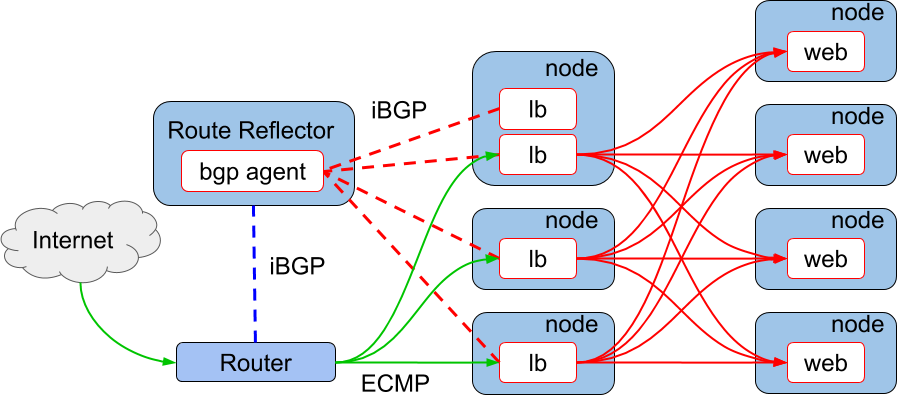
\includegraphics[width=0.8\columnwidth]{Figs/ecmp.png}
\caption{The proposed architecture of load balancer redundancy with ECMP}

\vspace{1mm}

\begin{minipage}{0.9\columnwidth}
   The traffic from the internet is distributed by the upstream router to multiple of load balancer(lb) pods using hash-based ECMP(the solid green line), after which distributed by the lb pods to web pods using Linux kernel's ipvs(the solid red line).
  The route toward a service IP is advertised to the route reflector(the dotted red line), after which advertised to the upstream router(the blue dotted line) using iBGP.
%  For the green lines, a service IP address is used. The red lines use the IP addresses of the overlay network. The blue line uses the IP addresses of the node network.
\end{minipage}

\label{fig:ecmp}
\end{figure}

While containerizing ipvs makes it runnable in any environment, it is essential to discuss how to route the ingress traffic to the ipvs container.
The author proposes redundant architecture using ECMP with BGP for proposed load balancer containers.

Fig.~\ref{fig:ecmp} shows a schematic diagram to explain redundancy architecture with ECMP for the proposed load balancer.
%
The ECMP is a functionality a router supports, where the router has multiple next hops with equal priority(cost) to a destination.
And the router generally distributes the traffic to the multiple next hops depending on the hash of five-tuples(source IP, destination IP, source port, destination port, protocol) of the flow.
The multiple next hops and their cost are often populated using the BGP protocol.
%
The notable benefit of the ECMP setup is its scalability.
All the load balancers that claims as the next hop is active, i.e., all of them are utilized to increase the performance level.
Since the traffic from the internet is distributed by the upstream router, the overall throughput is, after all, limited by performance levels of the router.
However, in practice, there are a lot of cases where this architecture is beneficial.
For example, if a software load balancer is capable of handling 1 Gbps equivalent of traffic and the upstream router is capable of handling 10 Gbps, it still is worthwhile launching 10 of the software load balancer containers to fill up maximum throughput of the upstream router.

%
In the proposed redundant architecture, there exists a node with the knowledge of the overlay network as a route reflector.
A route reflector is a network component for BGP to reduce the number of peerings by aggregating the routing information\cite{rfc4456}.
In the proposed architecture the author uses it as a delegater for load balancer containers towards the upstream router.

The route reflector exists for a practical reason, i.e, to deal with the complexity due to the overlay network.
Since the upstream router normally has no knowledge of the overlay network and IP addresses used inside the Kubernetes clusters, a container must rely on SNAT on the node to communicate with the router.
The SNAT caused a problem when the author tried a set up without the route reflector, to co-host multiple load balancer containers for different services on a single node.
Because of the SNAT, the source IP addresses of multiple connections were translated into a single IP address possessed by the node.
The BGP agent on the router was confused by these connections and could not properly set up ECMP routes for separate services.
This was due to the fact that the BGP agent used in the experiment used only the source IP address of the connection to distinguish the BGP peer.

In addition to that, the route reflector brings another benefit.
The upstream router does not need to accept BGP sessions from containers with random IP addresses, but only from the route reflector with well known fixed IP address.
This is preferable in terms of security especially when a different organization administers the upstream router.

By using the route reflector, we can have the following benefits.
1) Each node can accommodate multiple load balancer containers. This was not possible when we tried to directly connect load balancers and the router through SNAT.
2) The router does not need to allow peering connections from random IP addresses that may be used by load balancer containers. Now, the router only need to have the reflector information in the BGP peer definition.

Since a standard Linux system is used for the route reflector, it can be configured as we like;
a) It can be configured to belong to the overlay network so that multiple BGP sessions from containers on a single node can be properly distinguished.
b) One can select a BGP agent that supports dynamic neighbor (or dynamic peer), where he only needs to define the IP range as a peer group and does away with specifying every possible IP that load balancers may use.
Although not shown in the Fig.~\ref{fig:ecmp}, it is possible to have another route reflector for redundancy purpose.

\FloatBarrier



\section{Implementation}

In this section the author discusses the implementation of the experimental system to prove the concept of \replaced{the}{our} proposed load balancers with ECMP redundancy in detail.

\subsection{Experimental system architecture}\label{sec:poc}

\begin{figure}[tb]
\centering
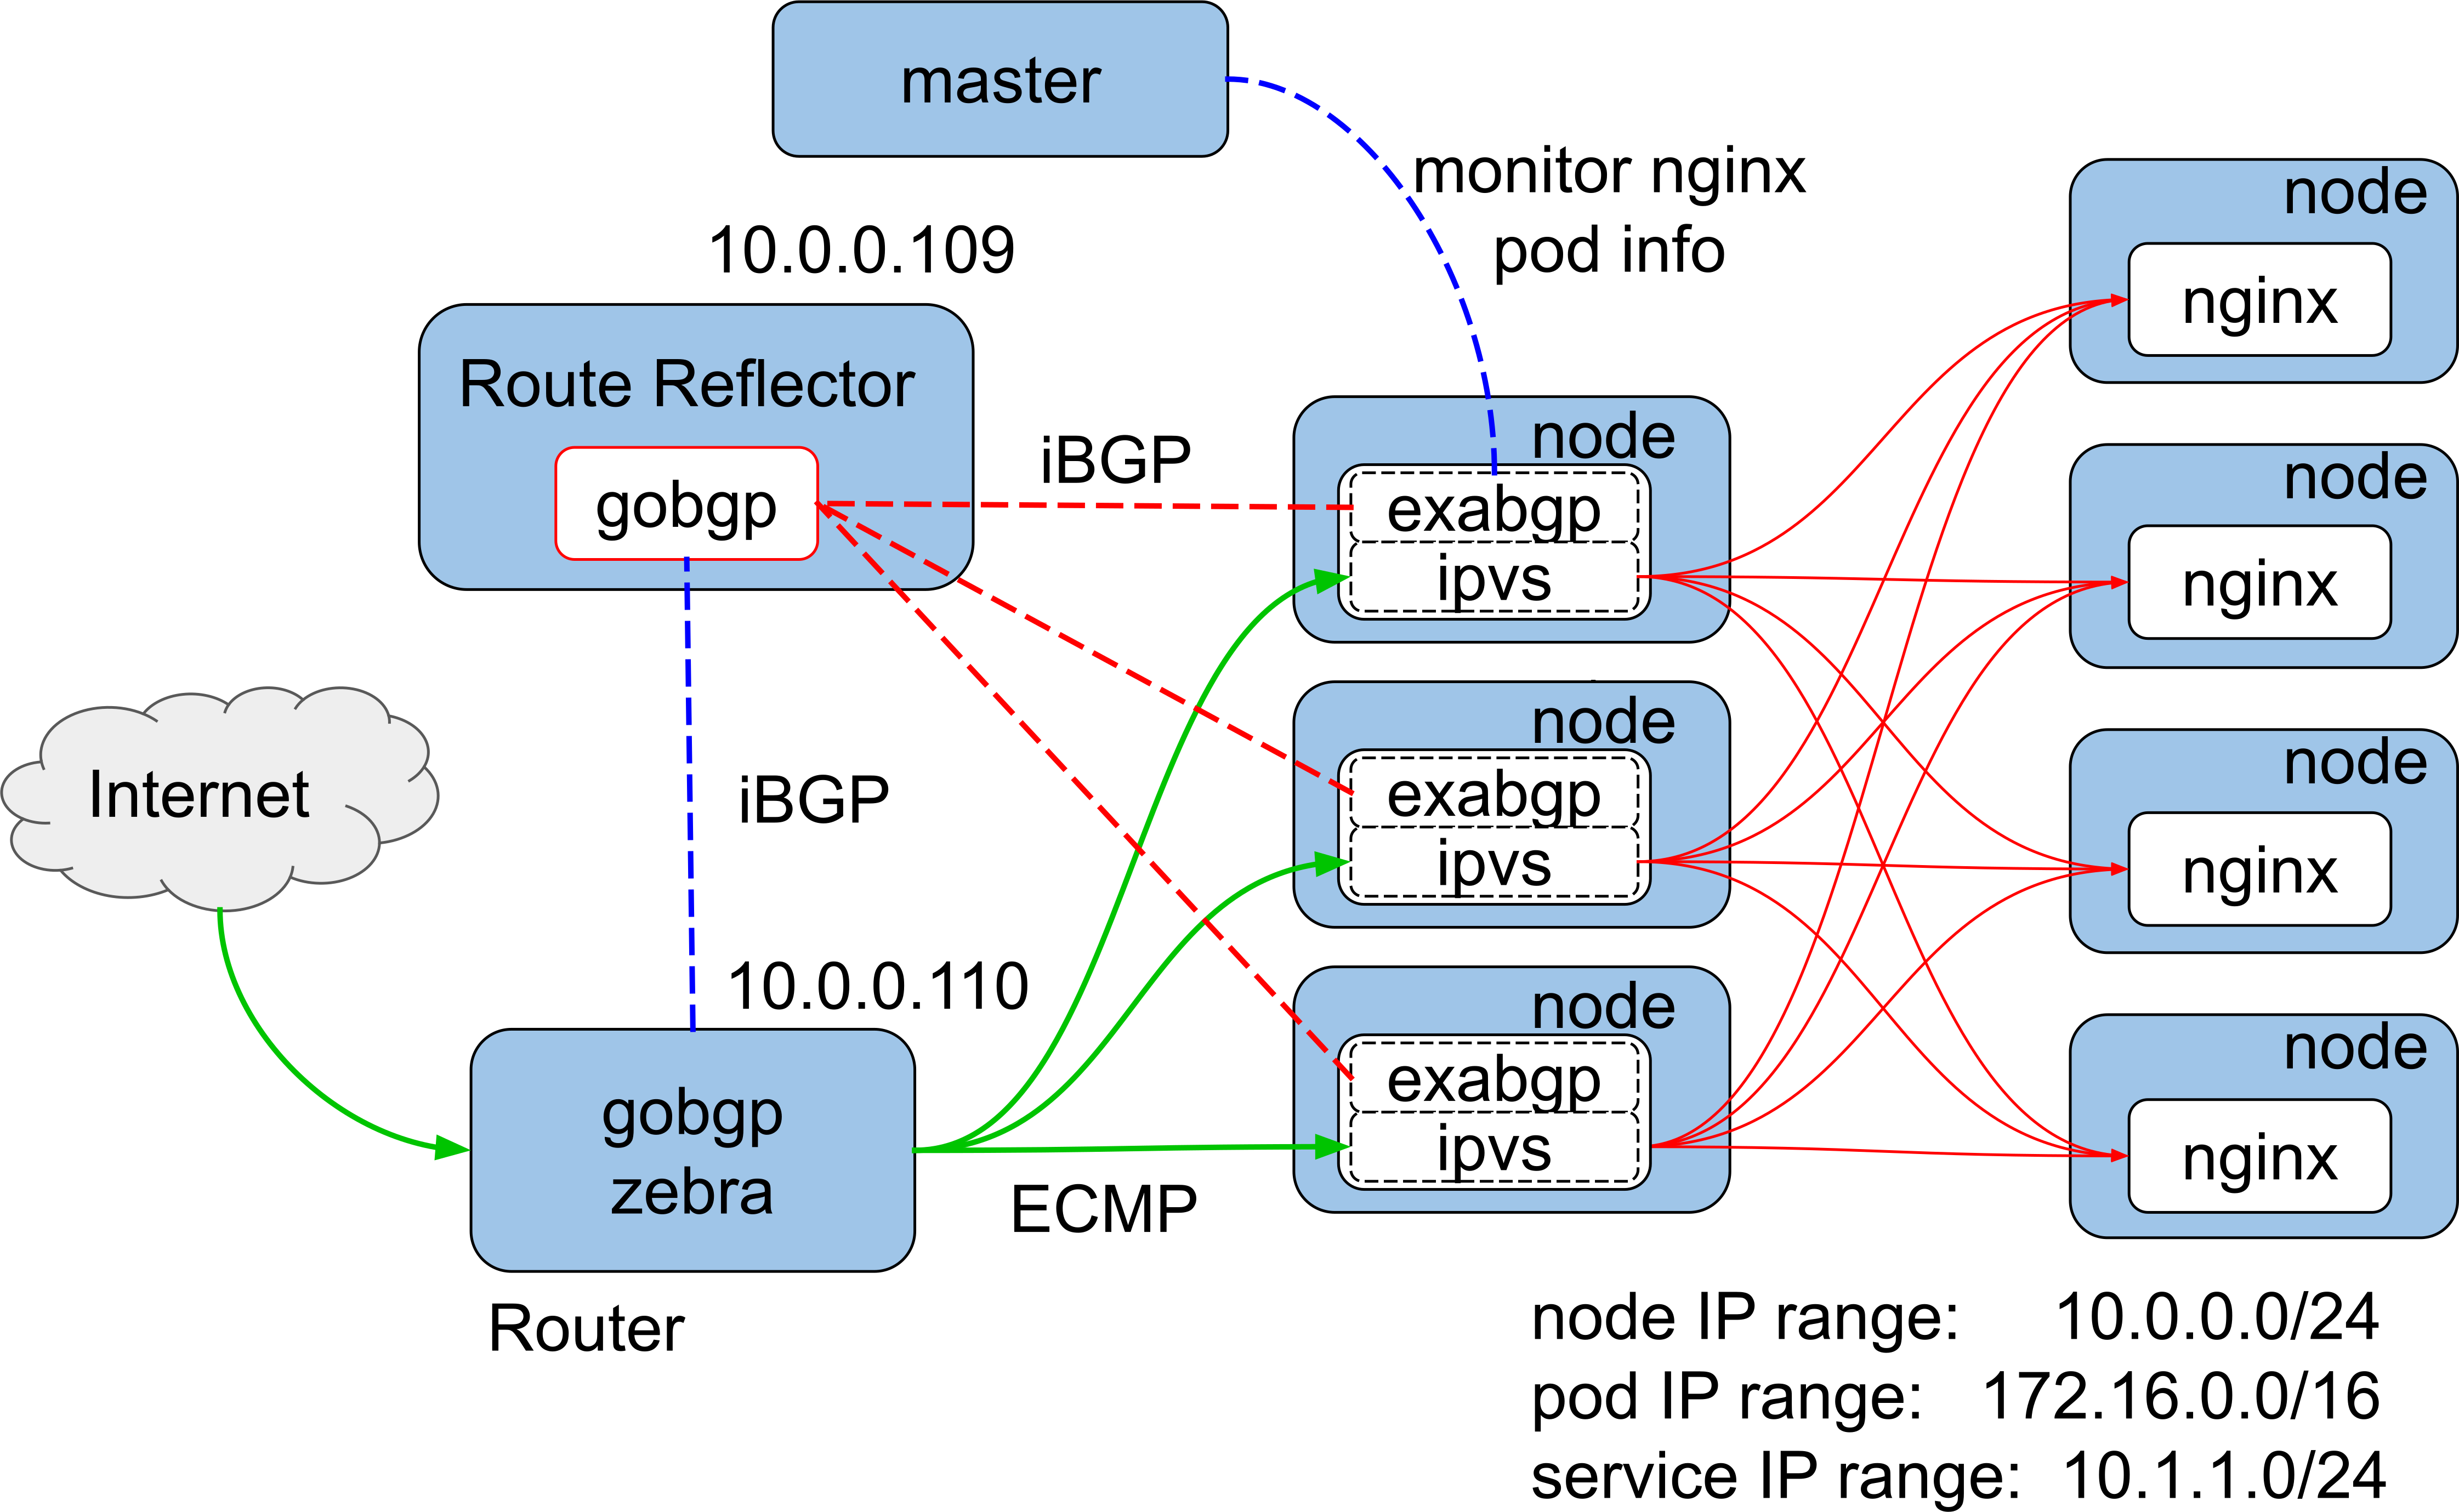
\includegraphics[width=0.8\columnwidth]{Figs/poc.png}

\par\bigskip
\centering
\begin{minipage}{0.9\columnwidth}
  \caption[An experimental container cluster with proposed redundant software balancers]{
    An experimental container cluster with proposed redundant software balancers.
    The master and nodes are configured as Kubernetes's master and nodes on top of conventional Linux systems, respectively.
    The route reflector and the upstream router are also conventional Linux systems.
    For the green lines, a service IP address is used. The red lines use the IP addresses of the overlay network. The blue line uses the IP addresses of the node network.
  }
  \label{fig:poc}
\end{minipage}

\end{figure}

Figure~\ref{fig:poc} shows the schematic diagram of proof of concept container cluster system with the proposed software load balancers.
%
Each load balancer pod consists of an exabgp \cite{exa-networks_2018} container and an ipvs container.
The ipvs container is responsible for distributing the traffic toward the service IP to web server (nginx) pods.
The IP address for nginx pods and load balancer pods are dynamically assigned upon launch of themselves from 172.16.0.0/16 address range.
The ipvs container monitors the availability of web server pods by consulting apiserver on the master node and manages the load balancing rule appropriately.
The exabgp container is responsible for advertising the route toward the service IP to the route reflector using BGP.
The route reflector aggregates the routing information advertised by load balancer pods and advertise them to the upstream router.
The upstream router updates its routing table according to the advertisement.

All the nodes and route reflector are configured using Debian 9.5 with self compiled linux-4.16.12 kernel.  
The author also used conventional Linux system as an upstream router for testing purpose, using the same OS as the nodes and route reflector.
The version of Linux kernel needed to be 4.12 or later to support hash based ECMP routing table.
The author also needed to enable kernel config option CONFIG\_IP\_ROUTE\_MULTIPATH \cite{ipsysctl} when compiling, and set the kernel parameter fib\_multipath\_hash\_policy=1 at run time.
Although in the actual production environment, proprietary hardware router with the highest throughput is usually deployed, one can still test some of the advanced features by using a conventional Linux system as the router.

\begin{table}[h]
  \centering
  \begin{tabular}{|l|c|c|c|}
    \hline
    & \multicolumn{1}{c|}{gobgpd} & \multicolumn{1}{c|}{exabgp} & \multicolumn{1}{c|}{bird} \\ \hline
    \begin{tabular}{l} Static route advertisement \end{tabular} & complex & simple & complex  \\ \hline
    \begin{tabular}{l} add-path support$^{*}$ \end{tabular} & Yes & No & Yes  \\ \hline
    \begin{tabular}{l} FIB manipulation \end{tabular} & Yes (through zebra) & No & Yes (Native) \\ \hline
    \begin{tabular}{l} Use case \end{tabular} & Router/Route reflector & Load balancer & Not used$^{**}$  \\ \hline
  \end{tabular}

  \par\bigskip
  \centering
  \begin{minipage}{0.9\columnwidth}
    \caption[Comparison of open source BGP agents]{
      Comparison of open source BGP agents.
      Open source BGP agents are compared in terms of the features required in the proposed systems. \par
      \small
      $^{*}$ \phantom{$^{*}$} The add-path is the feature to support multipath advertisement. \par
      $^{**}$ \phantom{$^{}$} Configuration of bird was more complex than other agents.
    }
    \label{table:bgp_agents}
  \end{minipage}
\end{table}

Table~\ref{table:bgp_agents} compares open source BGP agents in terms of required features for the proposed architecture.
Each load balancer {\em pod} needs to advertise a static route for the service IP to itself. 
For that purpose, exabgp is preferable because it only requires to add a line, e.g., \enquote{route Service\_IP next-hop Pod\_IP} in the configuration file.
The gobgpd and the bird require other client programs to inject the static route after the daemon itself is up and running.
For example, in the case of gobgpd, after launching gobgpd, a user is required to issue a command line, e.g., \enquote{gobgp global rib add Service\_IP/32 origin igp nexthop Pod\_IP community 100:50 -a ipv4}.
 (The gobgp is a client program to manage gobgpd.)
This is a bit complex and error-prone, especially when one needs to make sure the route injection is done inside a container.

As for the route reflector, add-path \cite{rfc7911} feature is needed for multi-path advertisement, which is supported by gobgpd.
For the upstream router Forwarding Information Base (FIB) manipulation \cite{exa-networks_2018} feature is needed, which is supported by gobgpd through zebra \cite{jakma2014introduction,osrg_gobgp_zebra}.
As a result, exabgp is used for the load balancer pods, gobgpd is used for the route reflector, and gobgpd and zebra are used for the upstream router.

The other features needed for the route reflector are a dynamic-neighbor feature to describe peer group as a range of IP address, and overlay network feature on the Linux system.
The configurations for the upstream router is summarised in Appendix~\ref{appendix:router_config}.
The configurations for the route reflector is summarised in Appendix~\ref{appendix:route_reflector_config}.

\subsection{Ipvs container}\label{sec:ipvs}

In order to demonstrate a software load balancer that is runnable in any environment, the author created Docker container using ipvs.
In addition to that, the proposed load balancer uses two other components, keepalived, and a controller.
These components are placed in a single Docker container image.
The ipvs is a Layer-4 load balancer capability, which is included in the Linux kernel 2.6.0 released in 2003 or later,
to distribute incoming Transmission Control Protocol (TCP) traffic to
{\em real servers}\footnote{The term, {\em real servers} refers to worker servers that will respond to incoming traffic,
in the original literature \cite{Zhang2000}. The author will also use this term in a similar way.} \cite{Zhang2000}.
For example, ipvs distributes incoming Hypertext Transfer Protocol (HTTP) traffic destined for a single destination IP address,
to multiple HTTP servers (e.g. Apache HTTP or nginx) running on multiple nodes in order to improve the performance of web services.
Keepalived is a management program that performs health checking for {\em real servers}
and manages ipvs balancing rules in the kernel accordingly.
It is often used together with ipvs to facilitate ease of use.
The controller is a daemon that periodically monitors the {\em pod} information on the master,
and it performs various actions when such information changes.
Kubernetes provides ingress controller framework as the Go Language (Golang) package to implement the controllers.
The author implemented a controller program that feeds {\em pod} state changes to keepalived
using this framework.

The proposed load balancer needs to dynamically reconfigure the ipvs balancing rules whenever {\em pods} are created or deleted. 
Figure~\ref{fig:ipvs-ingress-schem} is a schematic diagram of ipvs container to show the dynamic reconfiguration of the ipvs rules.
Two daemon programs, controller and keepalived, running in the container are illustrated.
The keepalived manages Linux kernel's ipvs rules depending on the ipvs.conf configuration file.
It can also periodically check the liveness of a {\em real server}
%
%\footnote{The term, {\em real servers} refers to worker servers that will respond to incoming traffic, 
%in the original literature \cite{Zhang2000}. We will also use this term in the similar way.}, 
which is represented as a combination of the IP addresses and port numbers of the target {\em pods}. 
If the health check to a {\em real server} fails, keepalived will remove that {\em real server} from the ipvs rules immediately.
The interval of the health check is typically 1 to several seconds and is arbitrarily determined by users.  

\begin{figure}[h]
  \centering
  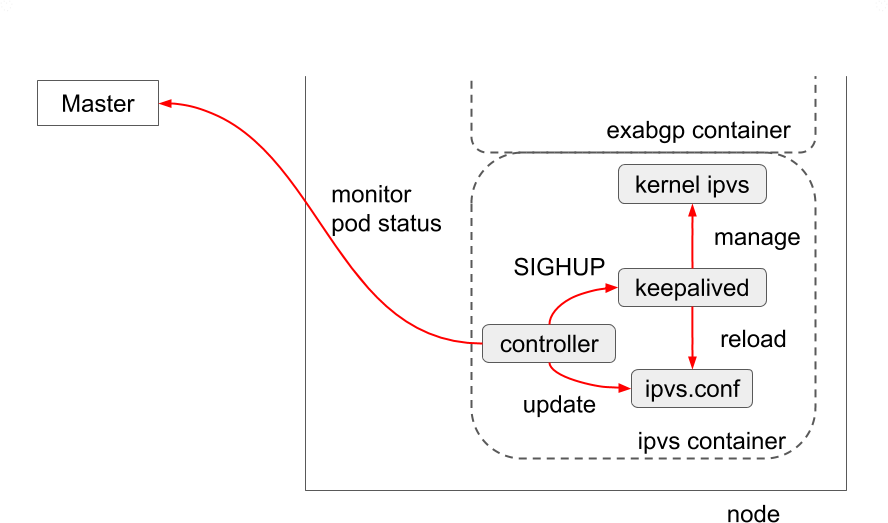
\includegraphics[width=0.8\columnwidth]{Figs/ipvs-ingress-schem}
  
    \par\bigskip
    \centering
    \begin{minipage}{0.9\columnwidth}
      \caption[Implementation of ipvs container]{
        Implementation of ipvs container.
        The controller checks the pod status every second, by consulting the master node.
        Upon a change of the status, the controller updates the ipvs.conf and sends SIGHUP to keepalived.
        The keepalived reload the ipvs.conf and updates the load balancing rules in the kernel correctly.
      }
      \label{fig:ipvs-ingress-schem}
    \end{minipage}
\end{figure}

Every second, the controller monitors information concerning the running {\em pods} of a web application in the Kubernetes cluster by consulting the apiserver running in the master through its API.
Whenever {\em pods} are created or deleted, the controller notices the change and automatically regenerate an appropriate ipvs.conf 
and issue SIGHUP to keepalived within a second.
Then, keepalived will reload the ipvs.conf, and modify the kernel's ipvs rules correctly depending on the result of the health check.

When a pod is terminated, existing connections are reset by the node kernel.
The SYN packets sent to a pod after termination, but before the ipvs rule update, will be answered with ICMP unreachable by the node.
In these cases, the client sees connection errors.
In order to avoid the connection errors to be seen by a human, HTTP client programs are required to re-initiate the connection.
However, since the load balancer rule update is within a second, these errors can be regarded as the tolerable rare exceptions even without such re-initiations.

The actual controller \cite{ktaka_ccmp_2017_826894} is implemented using the Kubernetes ingress controller \cite{K8sIngress2017} framework. 
By importing existing Golang package, \enquote{k8s.io/ingress/core/pkg/ingress}, the author could simplify the implementation, e.g. 
120 lines of code (Appendix~\ref{appendix:ingress_controller}).
%
Keepalived and the controller are placed in the docker image of ipvs container.
The ipvs is the kernel function and namespace separation for container has already been supported in the recent Linux kernel. 

Configurations for capabilities were needed when deploying the ipvs container: adding the CAP\_SYS\_MODULE capability 
to the container to allow the kernel to load required kernel modules inside a container, 
and adding CAP\_NET\_ADMIN capability to the container to allow keepalived to manipulate the kernel's ipvs rules. 
For the former case, the author also needed to mount the \enquote{/lib/module} of the node's file system on the container's file system.

\begin{figure}[h]
  \centering
  \begin{minipage}{0.7\columnwidth}
    \begin{lstlisting}[frame=single]
      virtual_server fwmark 1 {
        delay_loop 5
        lb_algo lc
        lb_kind NAT
        protocol TCP
        real_server 172.16.21.2 80 {
          uthreshold 20000
          TCP_CHECK {
            connect_timeout 5
        connect_port 80
          }
        }
        real_server 172.16.80.2 80 {
          uthreshold 20000
          TCP_CHECK {
            connect_timeout 5
            connect_port 80
          }
        }
      }
    \end{lstlisting}
  \end{minipage}

  \par\bigskip
    \centering
    \begin{minipage}{0.9\columnwidth}
      \caption[An example of ipvs.conf]{
        An example of ipvs.conf
        This configuration file is auto-generated by the controller.
        The controller periodically accesses the apiserver on the master node and constantly monitor the status of running pods.
      }
      \label{fig:ipvs.conf}
    \end{minipage}
\end{figure}

\begin{figure}[h]
  \centering
  \rule{\columnwidth}{0.4pt}
\begin{verbatim}
# kubectl exec -it IPVS-controller-4117154712-kv633 -- IPVSadm -L
IP Virtual Server version 1.2.1 (size=4096)
Prot LocalAddress:Port Scheduler Flags
  -> RemoteAddress:Port Forward Weight ActiveConn InActConn
FWM  1 lc
  -> 172.16.21.2:80      Masq    1      0          0         
  -> 172.16.80.2:80      Masq    1      0          0
\end{verbatim}
\rule{\columnwidth}{0.4pt}

  \par\bigskip
  \centering
  \begin{minipage}{0.9\columnwidth}
    \caption[Example of IPVS balancing rules]{
      Example of IPVS balancing rules.
      This shows the load balancing rule in a load balancer container.
      The packet that has FWM (fwmark)=1 will be forwarded to two real servers using the least connection (lc) balancing algorithm.
      The fwmark is a parameter that is only available inside a socket buffer in Linux kernel.
      The fwmark can be put and manipulated by the iptables program, once a socket buffer for a received packet is assigned by the kernel.
      }
    \label{fig:IPVS rule}
  \end{minipage}
\end{figure}

Figure~\ref{fig:ipvs.conf} and Figure~\ref{fig:IPVS rule} show an example of an ipvs.conf file 
generated by the controller and the corresponding IPVS load balancing rules, respectively.
Here, we can see that the packet with {\tt fwmark=1} \cite{BertHubert2002} is distributed 
to {\tt 172.16.21.2:80} and {\tt 172.16.80.2:80} 
using the masquerade mode (Masq) and 
the least connection (lc) \cite{Zhang2000} balancing algorithm.

\subsection{BGP software container}\label{sec:bgp}

\begin{figure}[tb]
  \centering
  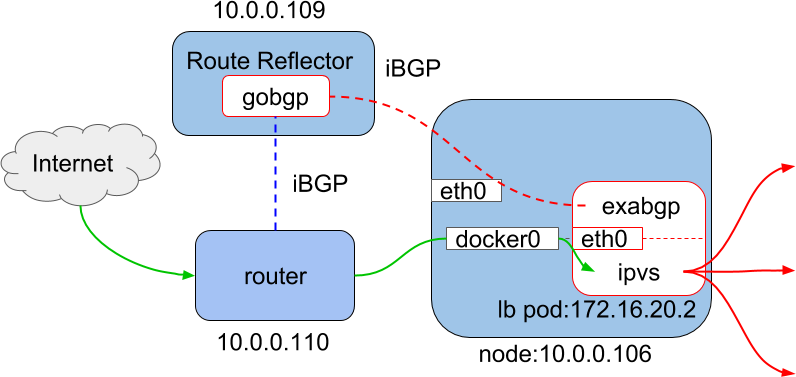
\includegraphics[width=0.8\columnwidth]{Figs/exabgp}
  
  \par\bigskip
  \centering
  \begin{minipage}{0.9\columnwidth}
    \caption[Network path by the exabgp container]{
      Network path by the exabgp container.
      The packets from Internet to service IPs, 10.1.1.0/24 are routed to the load balancer pod (green arrows) by the set of routing rules shown in Table~\ref{table:exabgp_setting}.
      And then the ipvs container forwards them to nginx pods (red arrows).
      The IP address of any pod is dynamically assigned from 172.16.0.0/16 when the pod is started. 
    }
    \label{fig:exabgp_schem}
  \end{minipage}

\end{figure}

\begin{table}
  \centering
  \begin{tabular}{lllr}
    \hline 
      \multicolumn{4}{l}{[BGP announcement]} \\
      \hspace{15 mm} & \multicolumn{2}{l}{route 10.1.1.0/24 next-hop 10.0.0.106} & ...(1) \\
      \multicolumn{4}{l}{[Routing in node net namespace]} \\
      \hspace{15 mm} & \multicolumn{2}{l}{ip netns exec node ip route replace 10.1.1.0/24 dev docker0} & ...(2) \\
      \multicolumn{4}{l}{[Accept as local]} \\
      \hspace{15 mm} & \multicolumn{2}{l}{ip route add local 10.1.1.0/24 dev eth0} & ...(3) \\
      \hline
  \end{tabular}
  
  \par\bigskip
  \centering
  \begin{minipage}{0.9\columnwidth}
    \caption[Required settings in the exabgp container]{
      Required settings in the exabgp container.
      (1) The node IP address, 10.0.0.106 is used as next-hop for the service IPs, 10.1.1.0/24, in BGP announcement.
      (2) In order to route the packets destined toward the service IP to the container, a routing rule to the dev docker0 is created in the node net namespace. 
      (3) A routing rule to accept the packets destined toward the service IPs,  as local is also required.
    }
    \label{table:exabgp_setting}
  \end{minipage}

\end{table}

In order to implement the ECMP redundancy, the author also containerized exabgp using Docker.
Figure~\ref{fig:exabgp_schem} shows a schematic diagram of the network path realized by the exabgp container.
As mentioned earlier, the author used exabgp as the BGP advertiser. 
The ingress traffic from the Internet is forwarded by ECMP routing table on the router to the node that hosts a load balancer pod.
And then it is routed to the load balancer pod according to the set of routing rules in Table~\ref{table:exabgp_setting}(2),(3).
After that the ipvs forwards them to nginx pods.
The IP address of any pod is dynamically assigned from 172.16.0.0/16 when the pod is started. 

Table~\ref{table:exabgp_setting} summarises some key settings required in the exabgp container to route the traffic to the ipvs container.
(1) In BGP announcements the node IP address, 10.0.0.106 is used as the next-hop for the service IPs, 10.1.1.0/24.
(2) Then on the node, in order to route the packets toward the service IPs to the ipvs container, 
a routing rule for 10.1.1.0/24 to the dev docker0 is created in the node net namespace. 
(3) A routing rule to accept the packets toward the service IPs as local is also required in the container net namespace. 
The configuration for exabgp is shown in Appendix~\ref{appendix:exabgp_config}.

\FloatBarrier


\section{Summary}

In this chapter, the author provided a discussion of load balancer architecture and its implementations suitable for container clusters.
%
First, the author discussed the problems of conventional architecture.
Since Kubernetes is dependent on external load balancers provided by the cloud infrastructures,
it failed to provide portability of a web application in environments where there was no supported load balancer.
Furthermore, the routes that ingress traffic from the internet follow were very complex and inefficient.

In order to alleviate these problems, the author proposed a cluster of software load balancers in containers.
The proposed load balancers utilized container technology and were managed by Kubernetes.
As a result, it is runnable on any environment including cloud infrastructures and on-premise data centers.
Furthermore, since Kubernetes manages load balancer containers, it can quickly scale the number of containers depending on the demand.
%
The author also discussed redundant architecture using ECMP with BGP for proposed load balancer containers.
By using the ECMP, the upstream router can route the ingress traffic to a cluster of load balancer containers in a redundant and scalable manner.
By using BGP, ECMP routing rules in the upstream router are automatically populated, upon the launch of load balancer containers.
The BGP and ECMP are both standard protocols supported by most of the commercial router products.

Thanks to the proposed load balancer, users become being able to set up routes to their web applications automatically, upon its launch, regardless of the infrastructures they use.  
This will greatly improve the portability of a web application and thereby enables migrations.






\chapter{Performance Evaluation}\label{chapter:Performance Evaluation}

In order to verify the feasibility of the proposed load balancer architecture, the author evaluated the performance of the load balancer with the following criteria;
(1) Performance analysis:
The author evaluated the basic characteristics of the load balancer using physical servers in the on-premise data center, and compared performance with those of iptables DNAT and nginx as a load balancer.
(2) Portability:
The author also carried out the same performance measurement in GCP and AWS to show the containerized ipvs load balancer is runnable in the cloud environment.
(3) Redundancy and Scalability:
The author evaluated ECMP functionality by monitoring routing table updates on the router when the new load balancer is added or removed.
The author also evaluated the aggregated performance level of the ECMP redundant load balancer.

\section{Performance analysis of proposed load balancer}

\subsubsection{Experimental conditions}

Throughput measurements were carried out in order to examine the basic characteristics of the containerized ipvs load balancer in an on-premise data center.
Figure~\ref{fig:benchmark-schem} shows the schematic diagram of the experimental setup for the measurement.
A benchmark program called wrk\cite{Glozer2016} were used.
Multiple nginx {\em pods} are deployed on multiple nodes as web servers in the Kubernetes cluster.
In each nginx {\em pod}, single nginx web server program that returns the IP address of the {\em pod} itself is running.
The author then launched ipvs pod and nginx pod as load balancers on one of the nodes, after that, performed the throughput measurement changing the number of the nginx web server pods.
On every Kubernetes node, there are iptables DNAT rules that function as an internal load balancer.
The author also measured throughput of this internal load balancer.
The throughput is measured by sending out HTTP requests from the wrk towards a load balancer and by counting the number of responses the benchmark client received.

\begin{figure}[h]
  \centering
  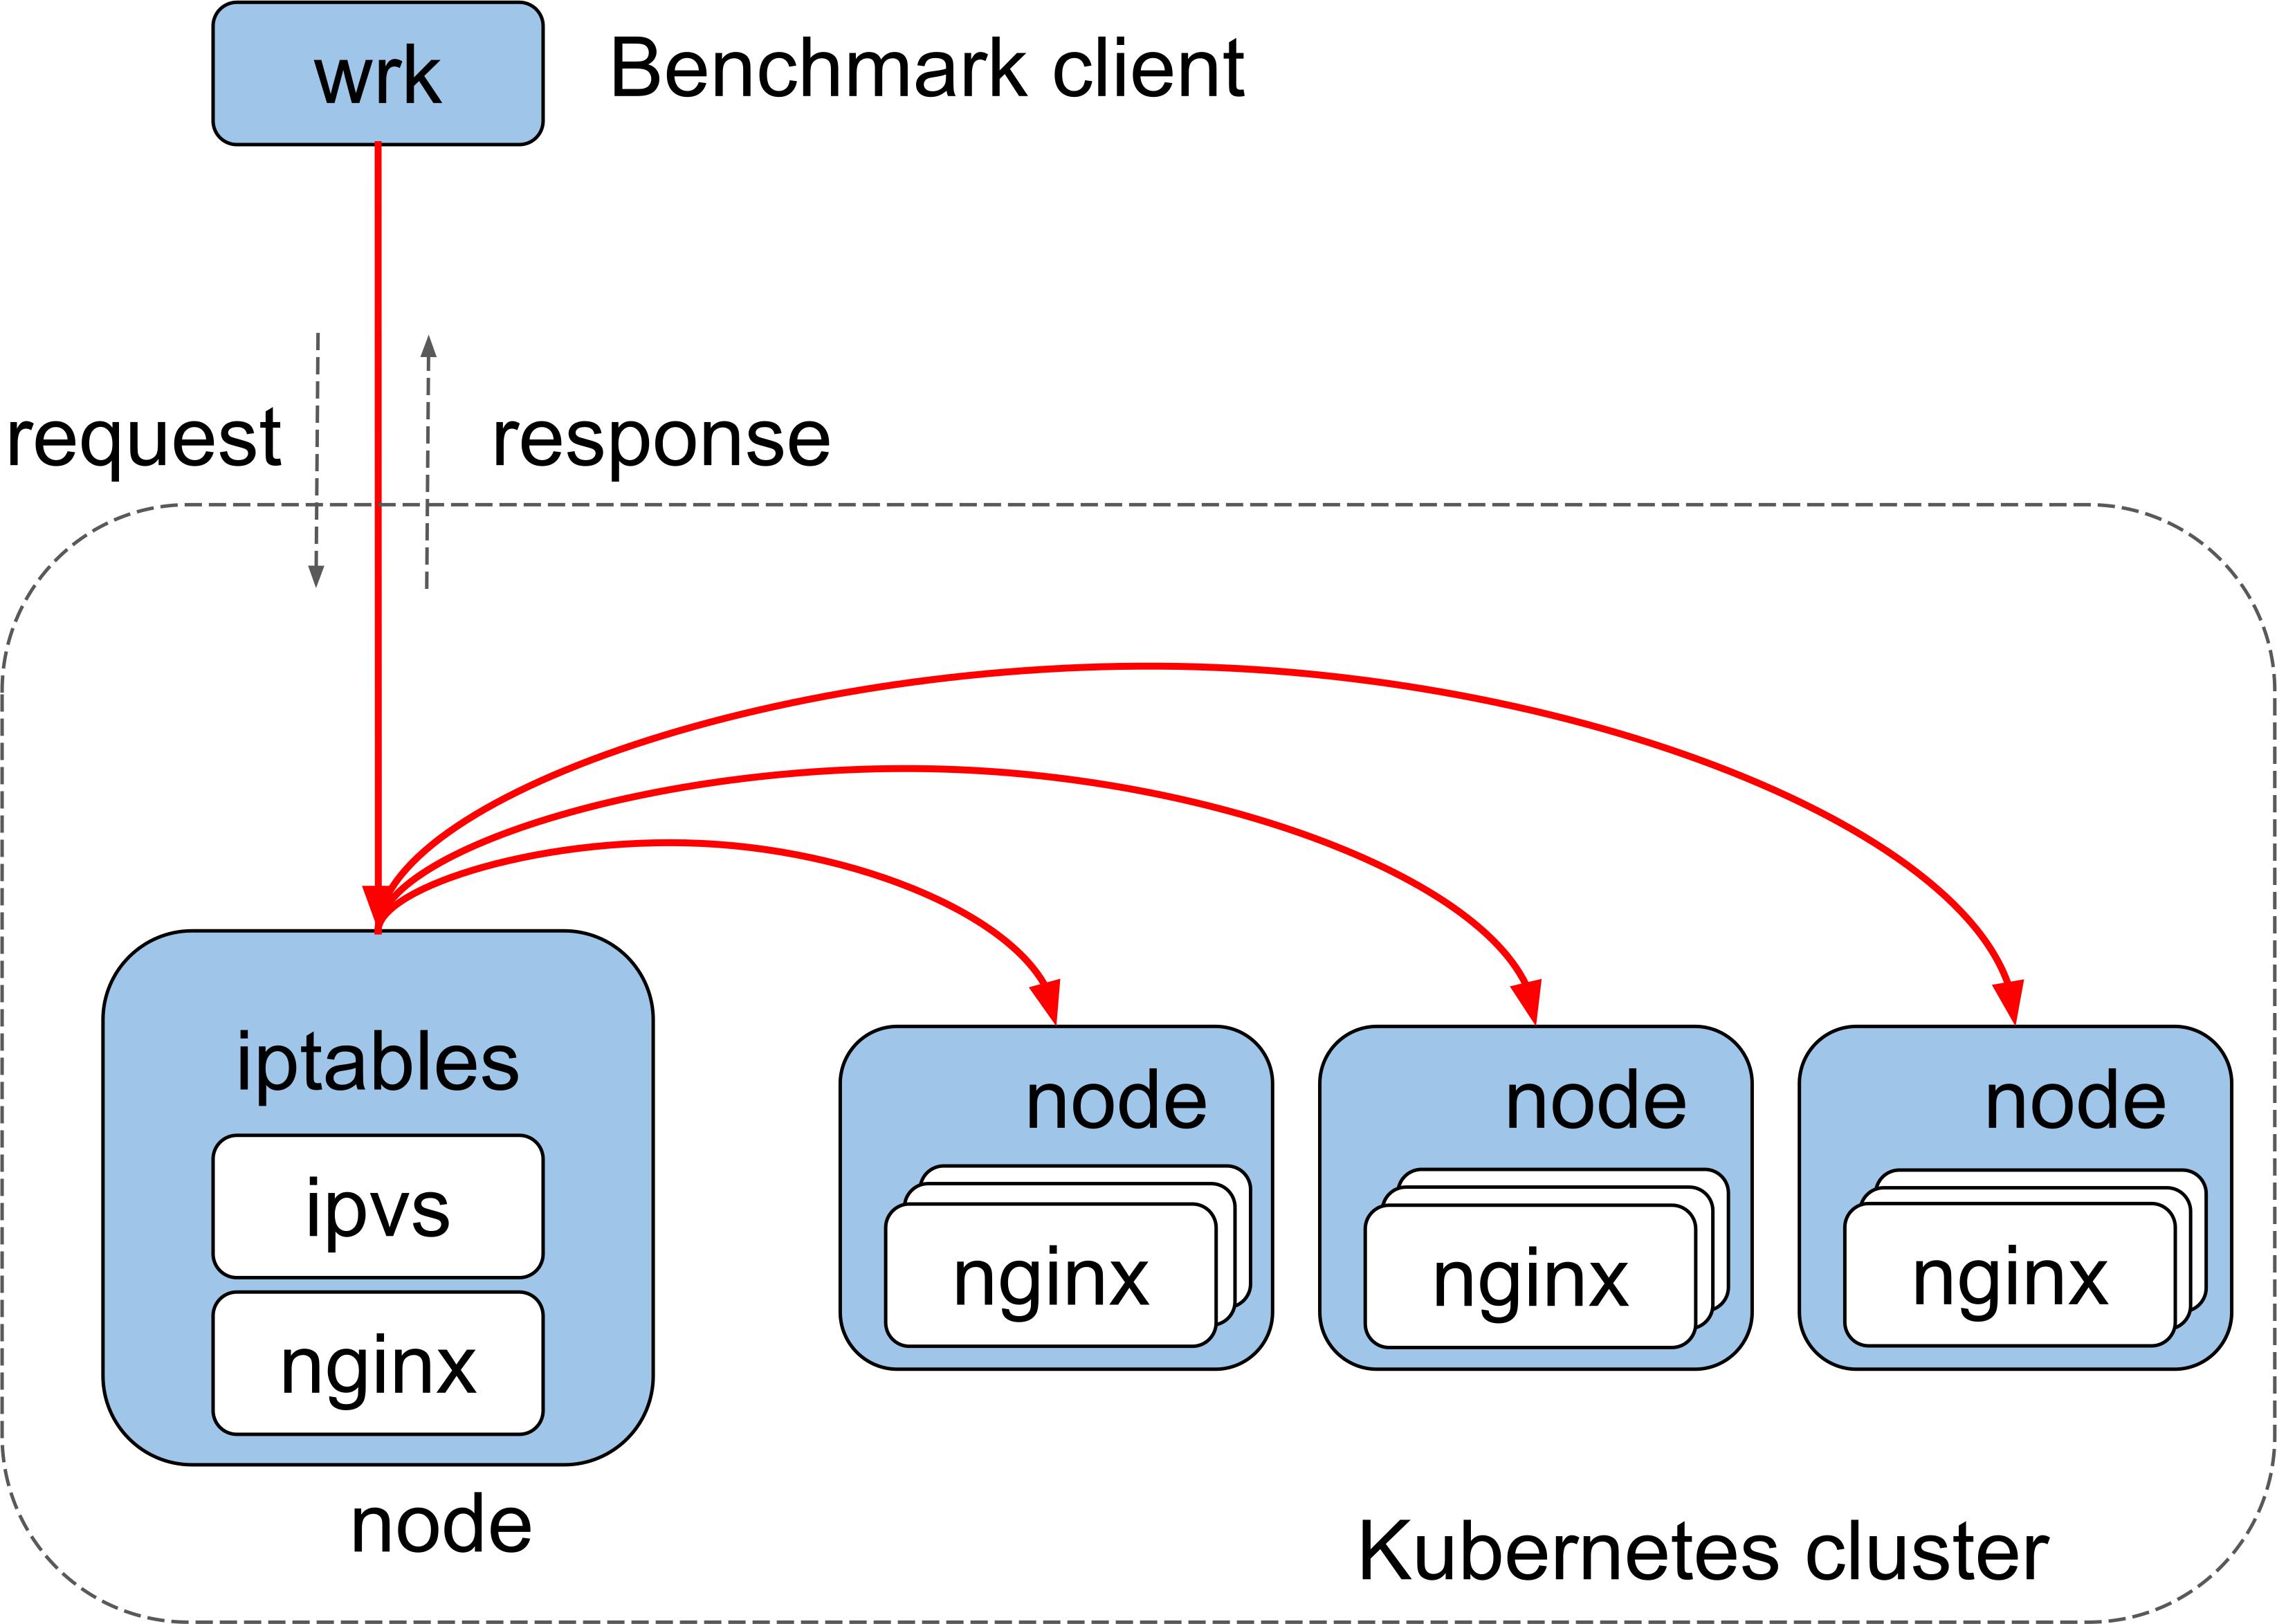
\includegraphics[width=0.8\columnwidth]{Figs/benchmark-schem}
  \par\bigskip
  \centering
  \begin{minipage}{0.9\columnwidth}
    \caption[Benchmark setup]{
      Benchmark setup.
      There are nodes on which nginx pods are deployed as web servers.
      There is another node where ipvs pod and nginx pod are deployed.
      Iptables DNAT rules exist on every Kubernetes node as an internal load balancer.
      Throughput measurements are performed against ipvs pod, nginx pod, and iptables DNAT rules.
      Each of the load balancers distributes the packets from the wrk to the nginx web servers.
      The response packets from the nginx web servers follow the same route as the request packets.  
    }
    \label{fig:benchmark-schem}
  \end{minipage}
\end{figure}

Table~\ref{fig:benchmark-schem} shows an example of the command-line for the benchmark program, wrk, and the corresponding output.
The command-line in Table~\ref{tab:bench_example} will generate 40 wrk program threads
and allow those threads to send out a total of 800 concurrent HTTP requests over the period of 30 seconds.
The output example shows information including per-thread statistics, error counts, throughput in [Request/sec] and data rate in [Transfer/sec].


{
%\setlength{\tabcolsep}{3em}
\renewcommand{\arraystretch}{1.1}

\begin{table}[h]

  \begin{subtable}{1\textwidth}
    \centering
    \begin{tabular}{lll}
      \hline
      &\verb|  wrk -c800 -t40 -d30s http://172.16.72.2:8888/       |& \\
      &\verb|      -c: concurrency, -t: # of thread, -d: duration  |& \\
      \hline
    \end{tabular}
    \centering\caption{Command line}
  \end{subtable}
 
\par\bigskip
 
  \begin{subtable}{1\textwidth}
    \centering
    \begin{tabular}{lll}
      \hline
      &\verb| Running 30s test @ http://10.254.0.10:81/            |& \\ 
      &\verb|  40 threads and 800 connections                      |& \\
      &\verb|  Thread Stats   Avg      Stdev     Max   +/- Stdev   |& \\
      &\verb|    Latency    15.82ms   41.45ms   1.90s    91.90\%   |& \\
      &\verb|    Req/Sec     4.14k   342.26     6.45k    69.24\%   |& \\
      &\verb|  4958000 requests in 30.10s, 1.14GB read             |& \\
      &\verb|  Socket errors: connect 0, read 0, write 0, timeout 1|& \\
      &\verb|Requests/sec: 164717.63                               |& \\
      &\verb|Transfer/sec:     38.86MB                             |& \\
      \hline
    \end{tabular}
    \centering\caption{Output example}
  \end{subtable}

  \centering
  \begin{minipage}{0.9\columnwidth}
    \caption[Benchmark command line and output example]{
      Benchmark command line and output example.
      (a) This command line will generate 40 wrk program threads and allow those threads to send out a total of 800 concurrent HTTP requests over the period of 30 seconds.
      (b) The output example shows information including per-thread statistics, error counts, throughput in [Request/sec] and data rate in [Transfer/sec].
      The throughput is 164717.63 [Request/sec] in this example.
    }
    \label{tab:bench_example}
  \end{minipage}
\end{table}
}

{
\setlength{\tabcolsep}{2em}
\renewcommand{\arraystretch}{1.1}

\begin{table}[h]
  \centering
  \begin{tabular}{ll}
    \hline 
    \multicolumn{2}{l}{[Hardware Specification]}   \\
    & CPU: Xeon E5-2450 2.10GHz (with 8 core, Hyper Threading) \\
    & Memory: 32GB \\
    & NIC: Broadcom BCM5720 with 4 rx-queues, 1 Gbps \\
    & (Node x 6, Load Balancer x 1, Client x 1) \\
%    \hline 
    & \\
%    \hline 
    \multicolumn{2}{l}{[Node Software]}  \\
    & OS: Debian 8.7, linux-3.16.0-4-amd64 \\
    & Kubernetes v1.10.6 \\
    & flannel v0.7.0 \\
    & etcd version: 3.0.15 \\
%    \hline 
    & \\
%    \hline 
    \multicolumn{2}{l}{[Container Software]}   \\
    & Keepalived: v1.3.2 (12/03,2016) \\
    & nginx : 1.11.1(load balancer), 1.13.0(web server) \\
    \hline
  \end{tabular}

  \centering
  \begin{minipage}{0.9\columnwidth}
    \caption[Hardware and software specifications]{
      Hardware and software specifications.
      The hardware had eight physical CPU cores and a network interface card (NIC) with four rx-queues.
    }
    \label{tab:hw_machine_spec}
  \end{minipage}
\end{table}
}

Table~\ref{tab:hw_machine_spec} shows hardware and software configuration used in the experiment.
The author used a total of eight servers; six servers for Nodes, one for the load balancer and one for the benchmark client, with all having the same hardware specifications.
The hardware had eight physical CPU cores and a network interface card (NIC) with four rx-queues.
The author configured nginx HTTP server to return a small HTTP content, the IP address of the {\em pod}, to make a relatively severe condition for load balancers. 
The size of the character string making up an IP address is limited to 15 bytes.

The author also investigated the performance level, varying two types of network conditions:
The first condition is the setting for multicore packet processing.
It is known that distributing handling of interrupts from the NIC and the subsequent IP protocol processing, among multiple cores impact the network performance.
To derive the best performance from load balancers, the author investigated how this setting would affect their performance levels.
The second condition is an overlay network setting\cite{Sill2016,Marmol2015}.
The overlay network is often used to build the Kubernetes cluster and therefore used in the experiment.
Flannel\cite{CoreOSFlannel} is one of the popular overlay network technologies. 
The author compared the performance levels of three backends settings\cite{CoreOSFlannelBackend} of flannel, i.e., operating modes, to find the best setting.

\FloatBarrier

\subsubsection{Effect of multicore processing}

Figure~\ref{fig:ipvs_mcore_proccessing} shows the result of the throughput measurement for the ipvs load balancer with different multicore processing settings.
Since hardware used in the experiment has a NIC with four rx-queues, and a CPU with eight cores,
the setting \enquote{(RSS, RPS) = (on, off)} uses four cores and \enquote{(RSS, RPS) = (off, on)} uses eight cores for packet processing.
For the setting \enquote{(RSS, RPS) = (off, off)}, only one core is used for the packet processing.

There is a general trend in the throughput result, where the throughput linearly increases as the number of nginx {\em pod}s increases and then it eventually saturates.
For example, if we look at the red line in the Figure~\ref{fig:ipvs_mcore_proccessing}, the throughput increases almost linearly as the number of the nginx pods(web servers) increases from 1 to around 14, and then saturates.
The increase indicates that the load balancer functions properly, as the load balancer increased throughput by distributing HTTP requests to multiple of the web servers.
%
The saturated throughput indicates the maximum performance level of the load balancer, which could be determined either by network bandwidth between the benchmark client machine and the load balancer node, or CPU performance levels of these machines.
%
The maximum performance levels are dependent on the number of cores used for packet processing.
Throughput is highest for the setting with eight cores (rps = on), followed by four cores (rss = on), then single core (none).
This indicates that the more cores are used, the better the throughput is.

Figure~\ref{fig:iptables_mcore_proccessing} shows the result of the throughput measurement for iptables DNAT as a load balancer, with different multicore processing settings.
As is the case for the ipvs result, there is a general trend where the throughput increases as the number of nginx {\em pod}s increases and then it eventually saturates.
Also, throughput is highest for the setting with eight cores (rps = on), followed by four cores (rss = on), then single core (none).
%
The saturated performance levels of iptables DNAT and ipvs are the same for the condition with eight cores (rss = on). 
The saturated performance levels of iptables DNAT are higher than those of ipvs, for the conditions with four cores (rss = on) and single core (none).

\begin{figure}[h]
  \centering
  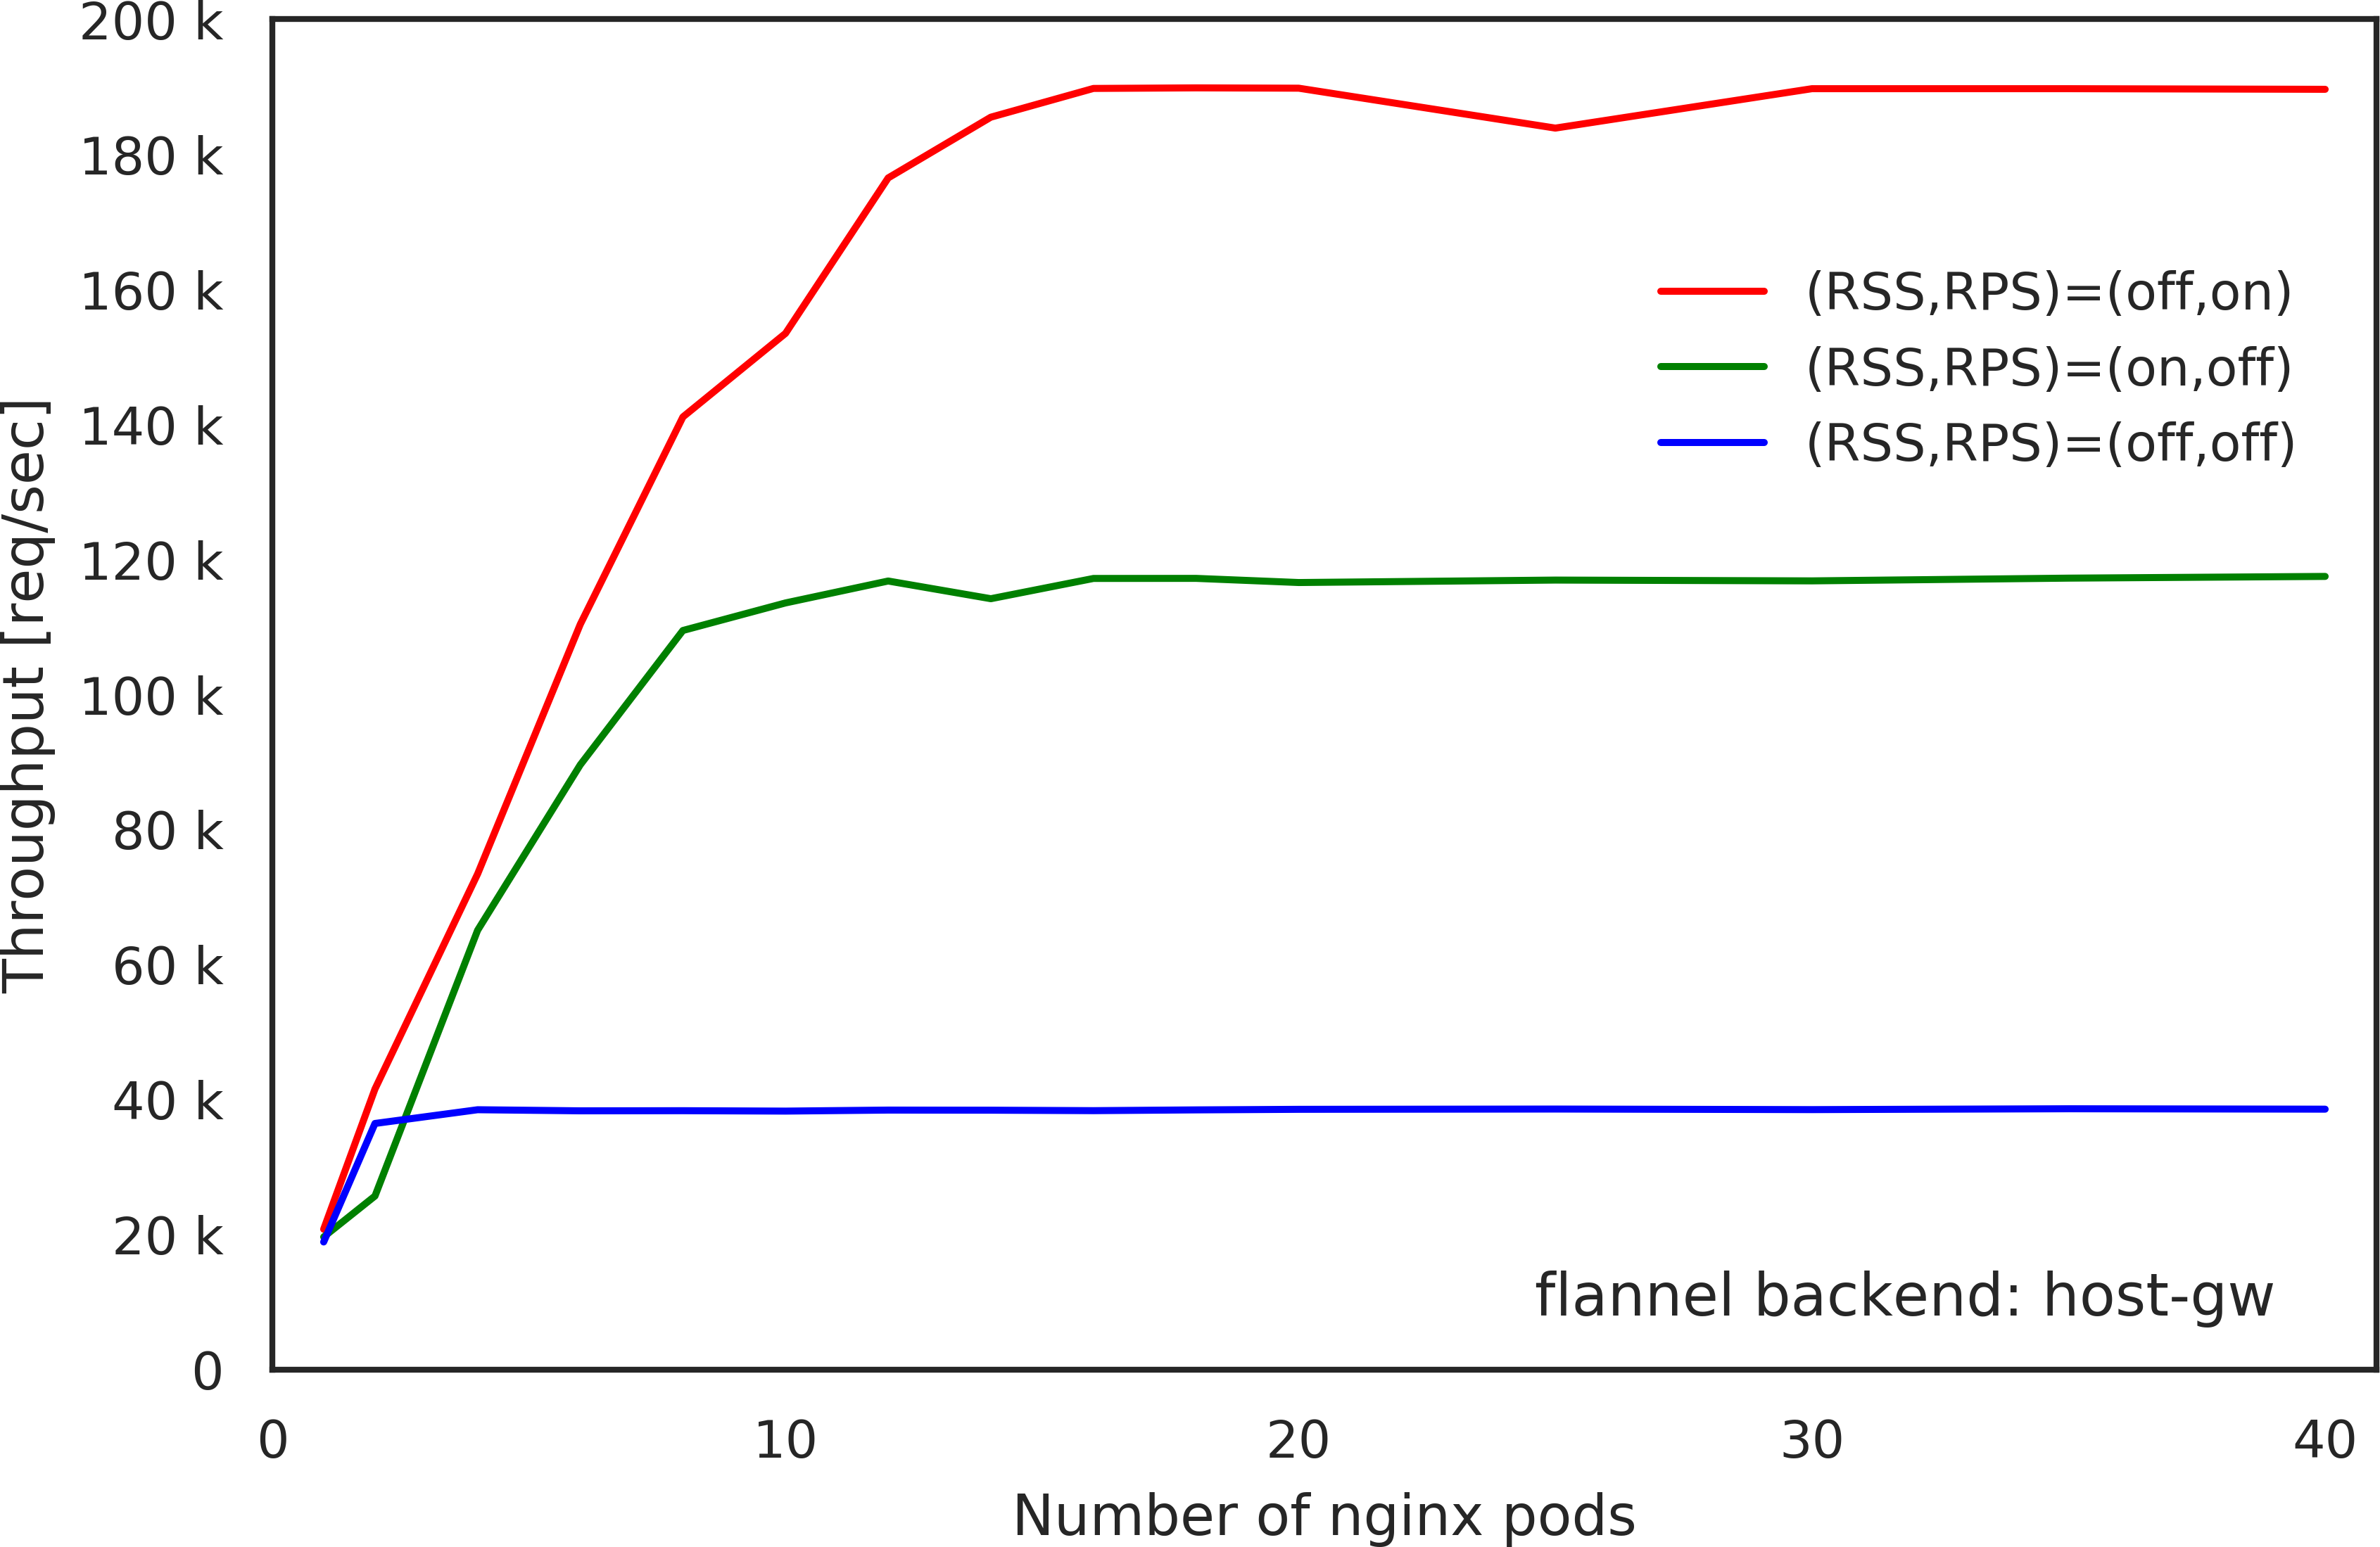
\includegraphics[width=0.75\columnwidth]{Figs/ipvs_mcore_proccessing}
  \par\bigskip
  \centering
  \begin{minipage}{0.9\columnwidth}
    \caption[Effect of multicore packet processing on ipvs throughput]{
Effect of multicore packet processing on ipvs throughput.
Throughput linearly increases as the number of nginx {\em pod}s increases and then it eventually saturates.
The throughput is highest for the setting with eight cores (rps = on), followed by four cores (rss = on), then single core (none).
    }
    \label{fig:ipvs_mcore_proccessing}
  \end{minipage}
\end{figure}


\begin{figure}[h]
  \centering
  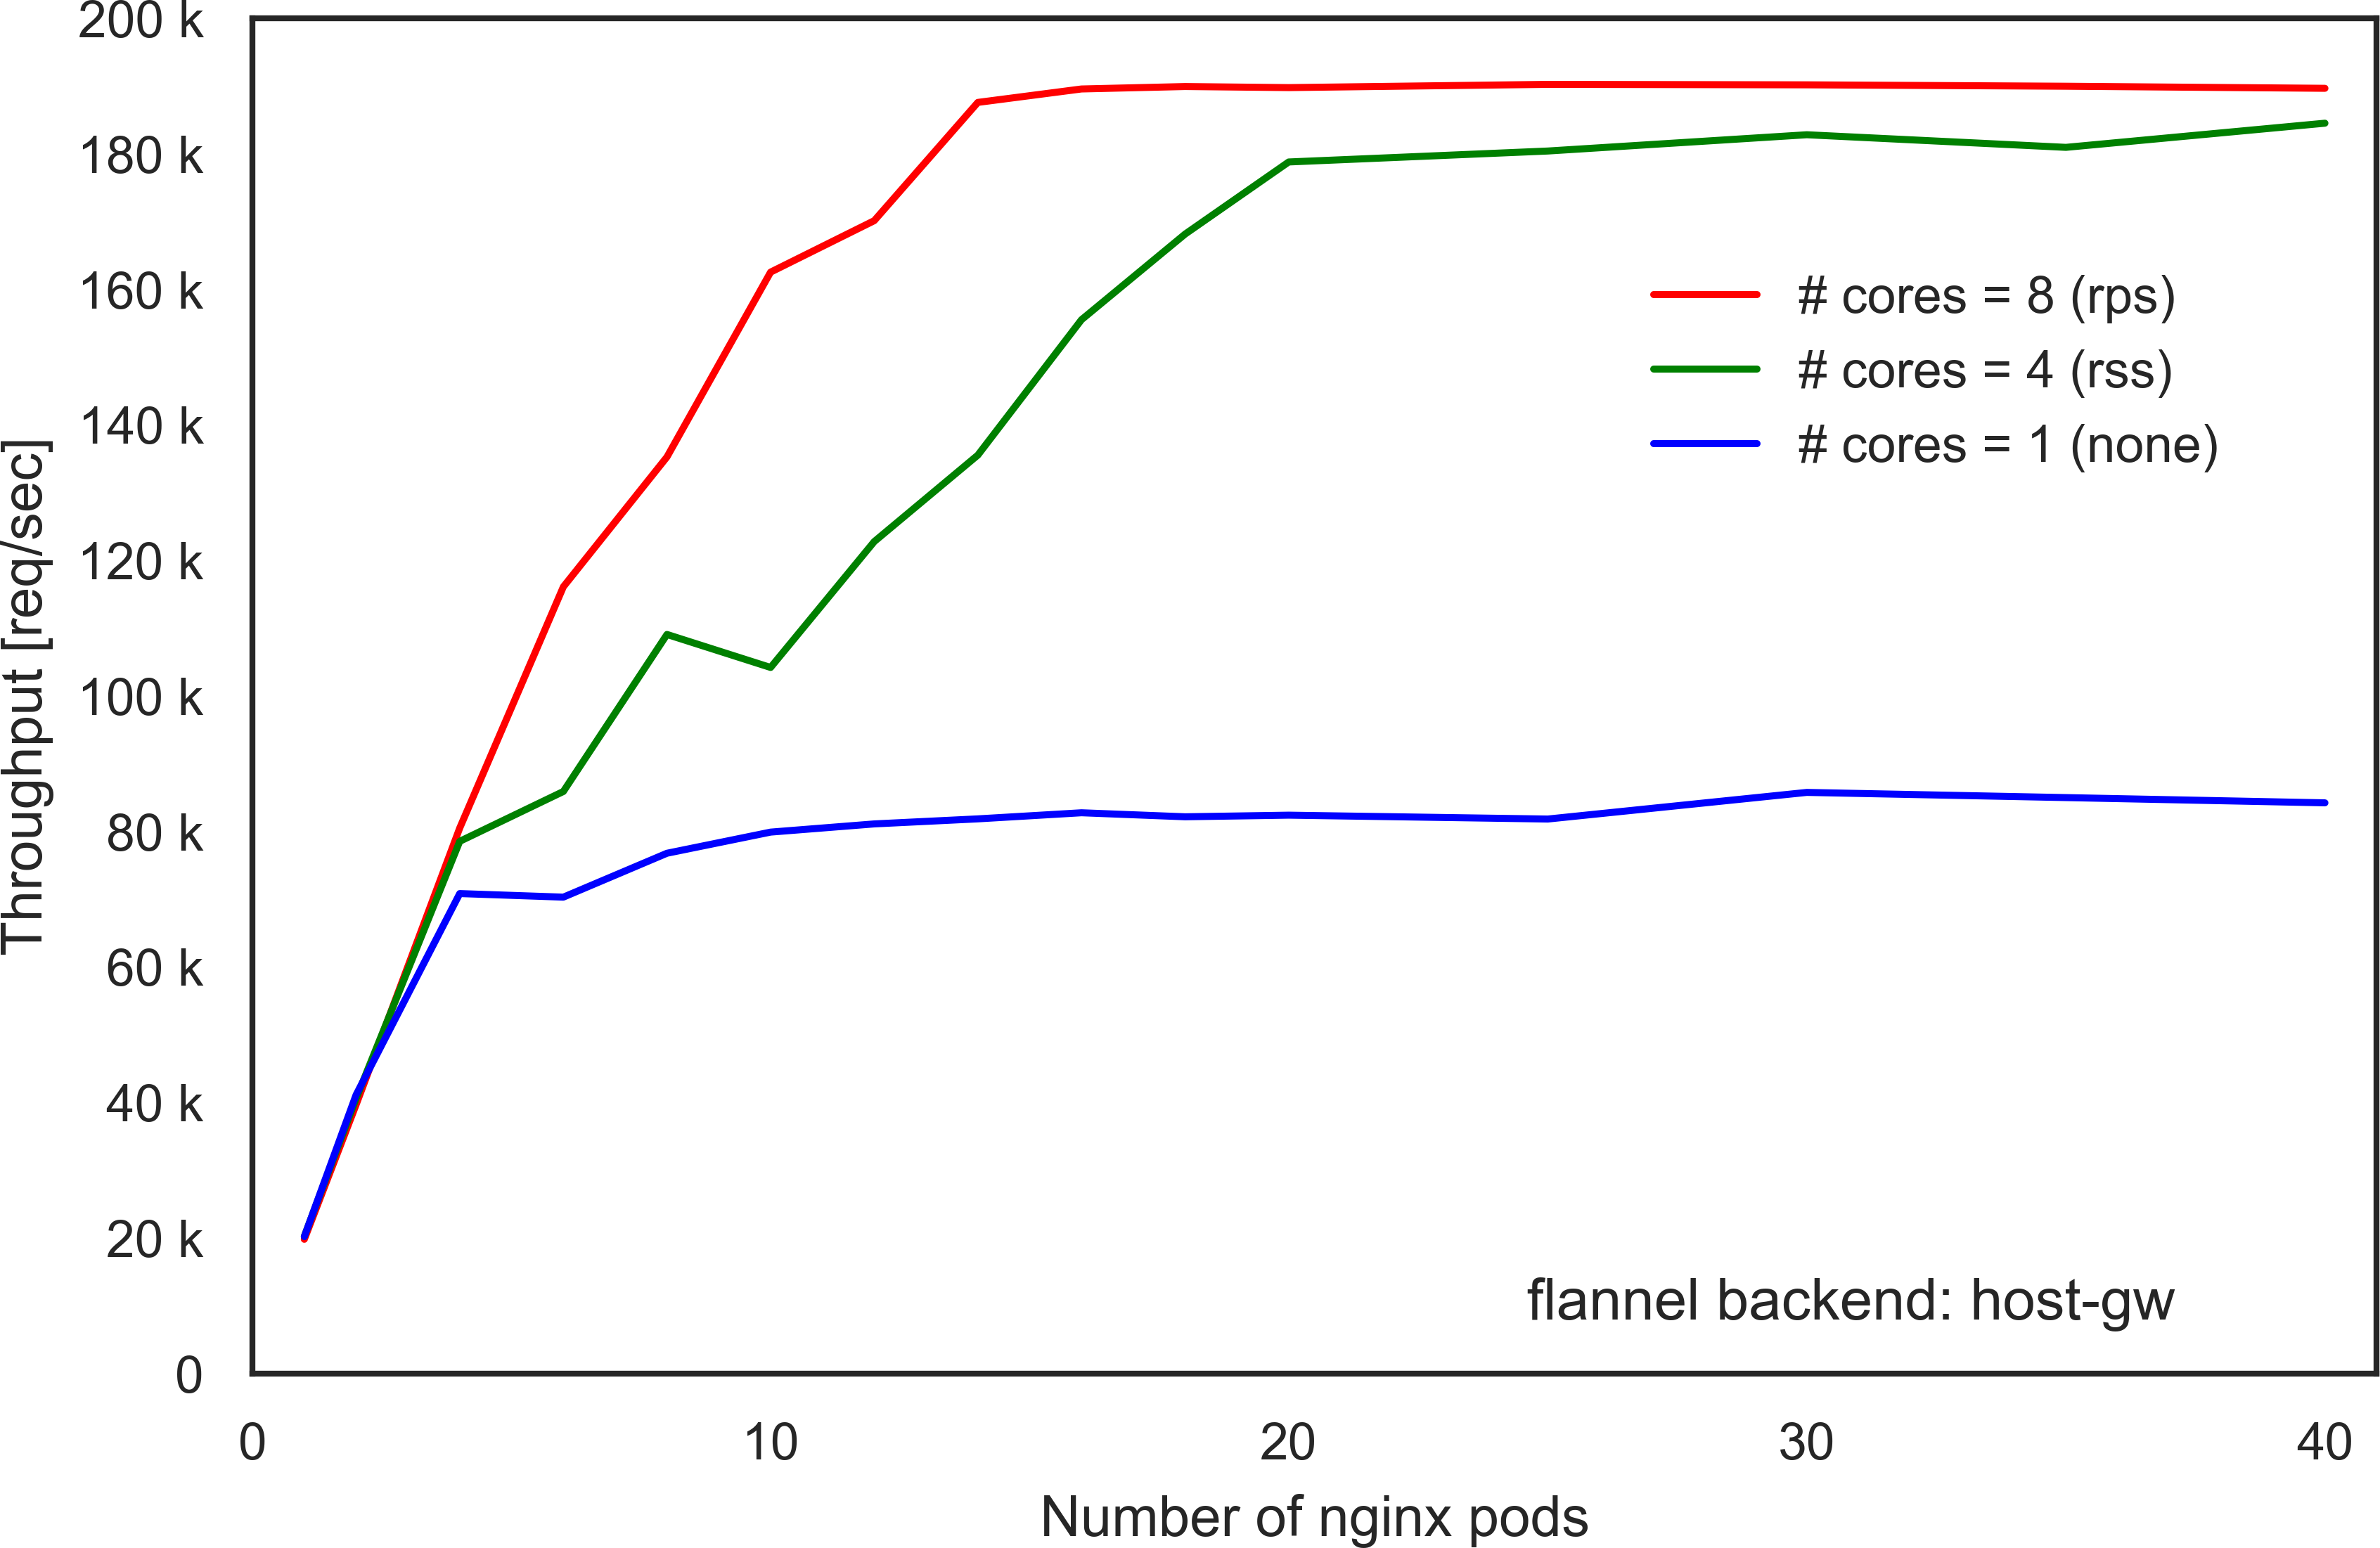
\includegraphics[width=0.75\columnwidth]{Figs/iptables_mcore_proccessing}
  \par\bigskip
  \centering
  \begin{minipage}{0.9\columnwidth}
    \caption[Effect of multicore packet processing on iptables DNAT throughput]{
Effect of multicore packet processing iptables DNAT throughput.
Throughput linearly increases as the number of nginx {\em pod}s increases and then it eventually saturates.
The throughput is highest for the setting with eight cores (rps is on), followed by four cores (rss is on), then single core (none).
    }
    \label{fig:iptables_mcore_proccessing}
  \end{minipage}
\end{figure}


\FloatBarrier

\subsubsection{Effect of overlay network}

Figure~\ref{fig:ipvs_flannel_mode} shows the ipvs throughput results for different overlay network settings.
The author used the flannel for the overlay network.
Flannel has three backend modes, host-gw, vxlan and udp, and the throughput for each setting are compared.

Except for the udp backend mode case, a general trend can be clearly seen, i.e., the throughput linearly increases as the number of nginx {\em pod} increases, and then it eventually saturates.
Among the flannel backend mode types, the host-gw mode where no encapsulation is conducted shows the highest performance level,
followed by the vxlan mode where the Linux kernel encapsulates the Ethernet frame.
The udp mode where flanneld itself encapsulates the IP packet shows significantly lower performances levels.

Figure~\ref{fig:iptables_flannel_mode} shows throughput results of the iptables DNAT as a load balancer for different overlay network settings.
The same characteristics can be seen for the iptables DNAT, although the performance level of the iptables DNAT for udp mode is slightly better than that of ipvs.

As is shown here, overlay network settings greatly affect the performance level.
The author considers the host-gw mode is the best, the vxlan tunnel the second best and the udp tunnel mode unusable.
In environments where containers need to communicate with each other via a gateway that has no knowledge of overlay network, the backend modes with tunneling are inevitable, which is often the case in cloud environments. 
The author used vxlan mode for the experiments conducted in cloud environments and host-gw mode for the rest of the experiments conducted in on-premise data centers.

\begin{figure}[h]
  \centering
  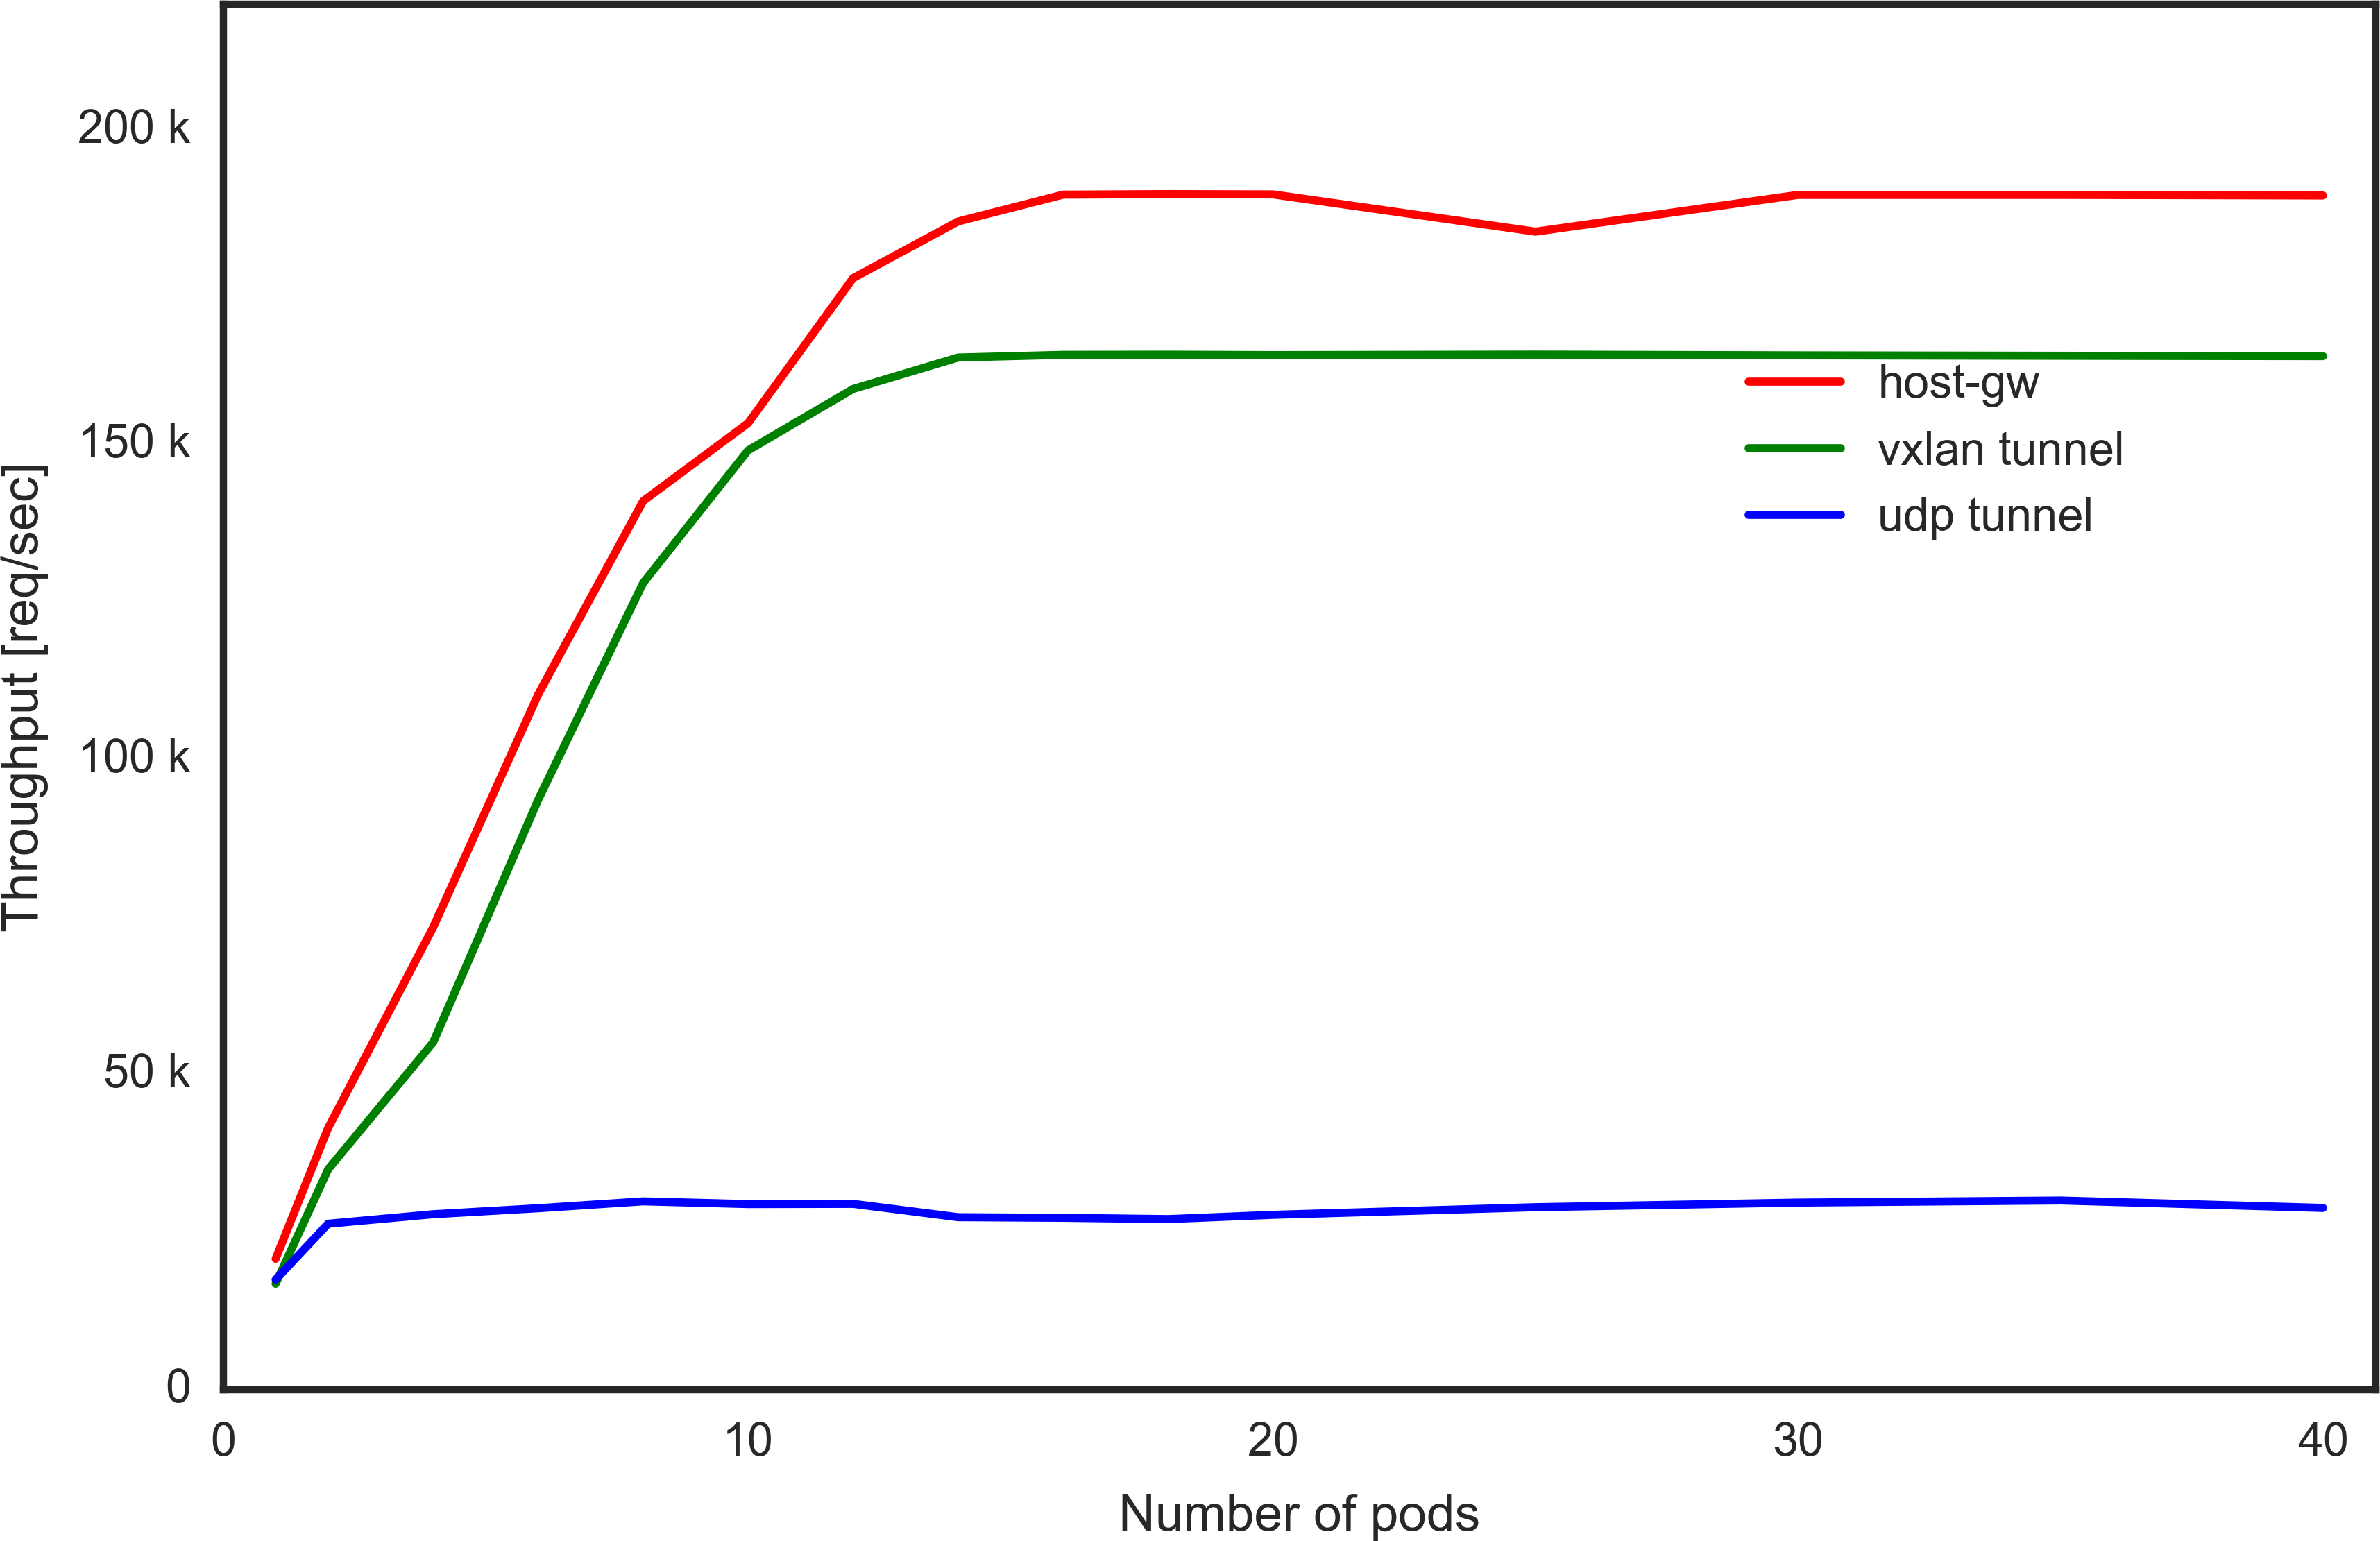
\includegraphics[width=0.75\columnwidth]{Figs/ipvs_flannel_mode}

  \par\bigskip
  \centering
  \begin{minipage}{0.9\columnwidth}
    \caption[Effect of flannel backend modes on ipvs throughput]{
      Effect of flannel backend modes on ipvs throughput.
      The host-gw mode shows the highest performance level, followed by the vxlan mode.
      The udp mode shows significantly lower performances levels.
    }
    \label{fig:ipvs_flannel_mode}
  \end{minipage}
\end{figure}

\begin{figure}[h]
    \centering
    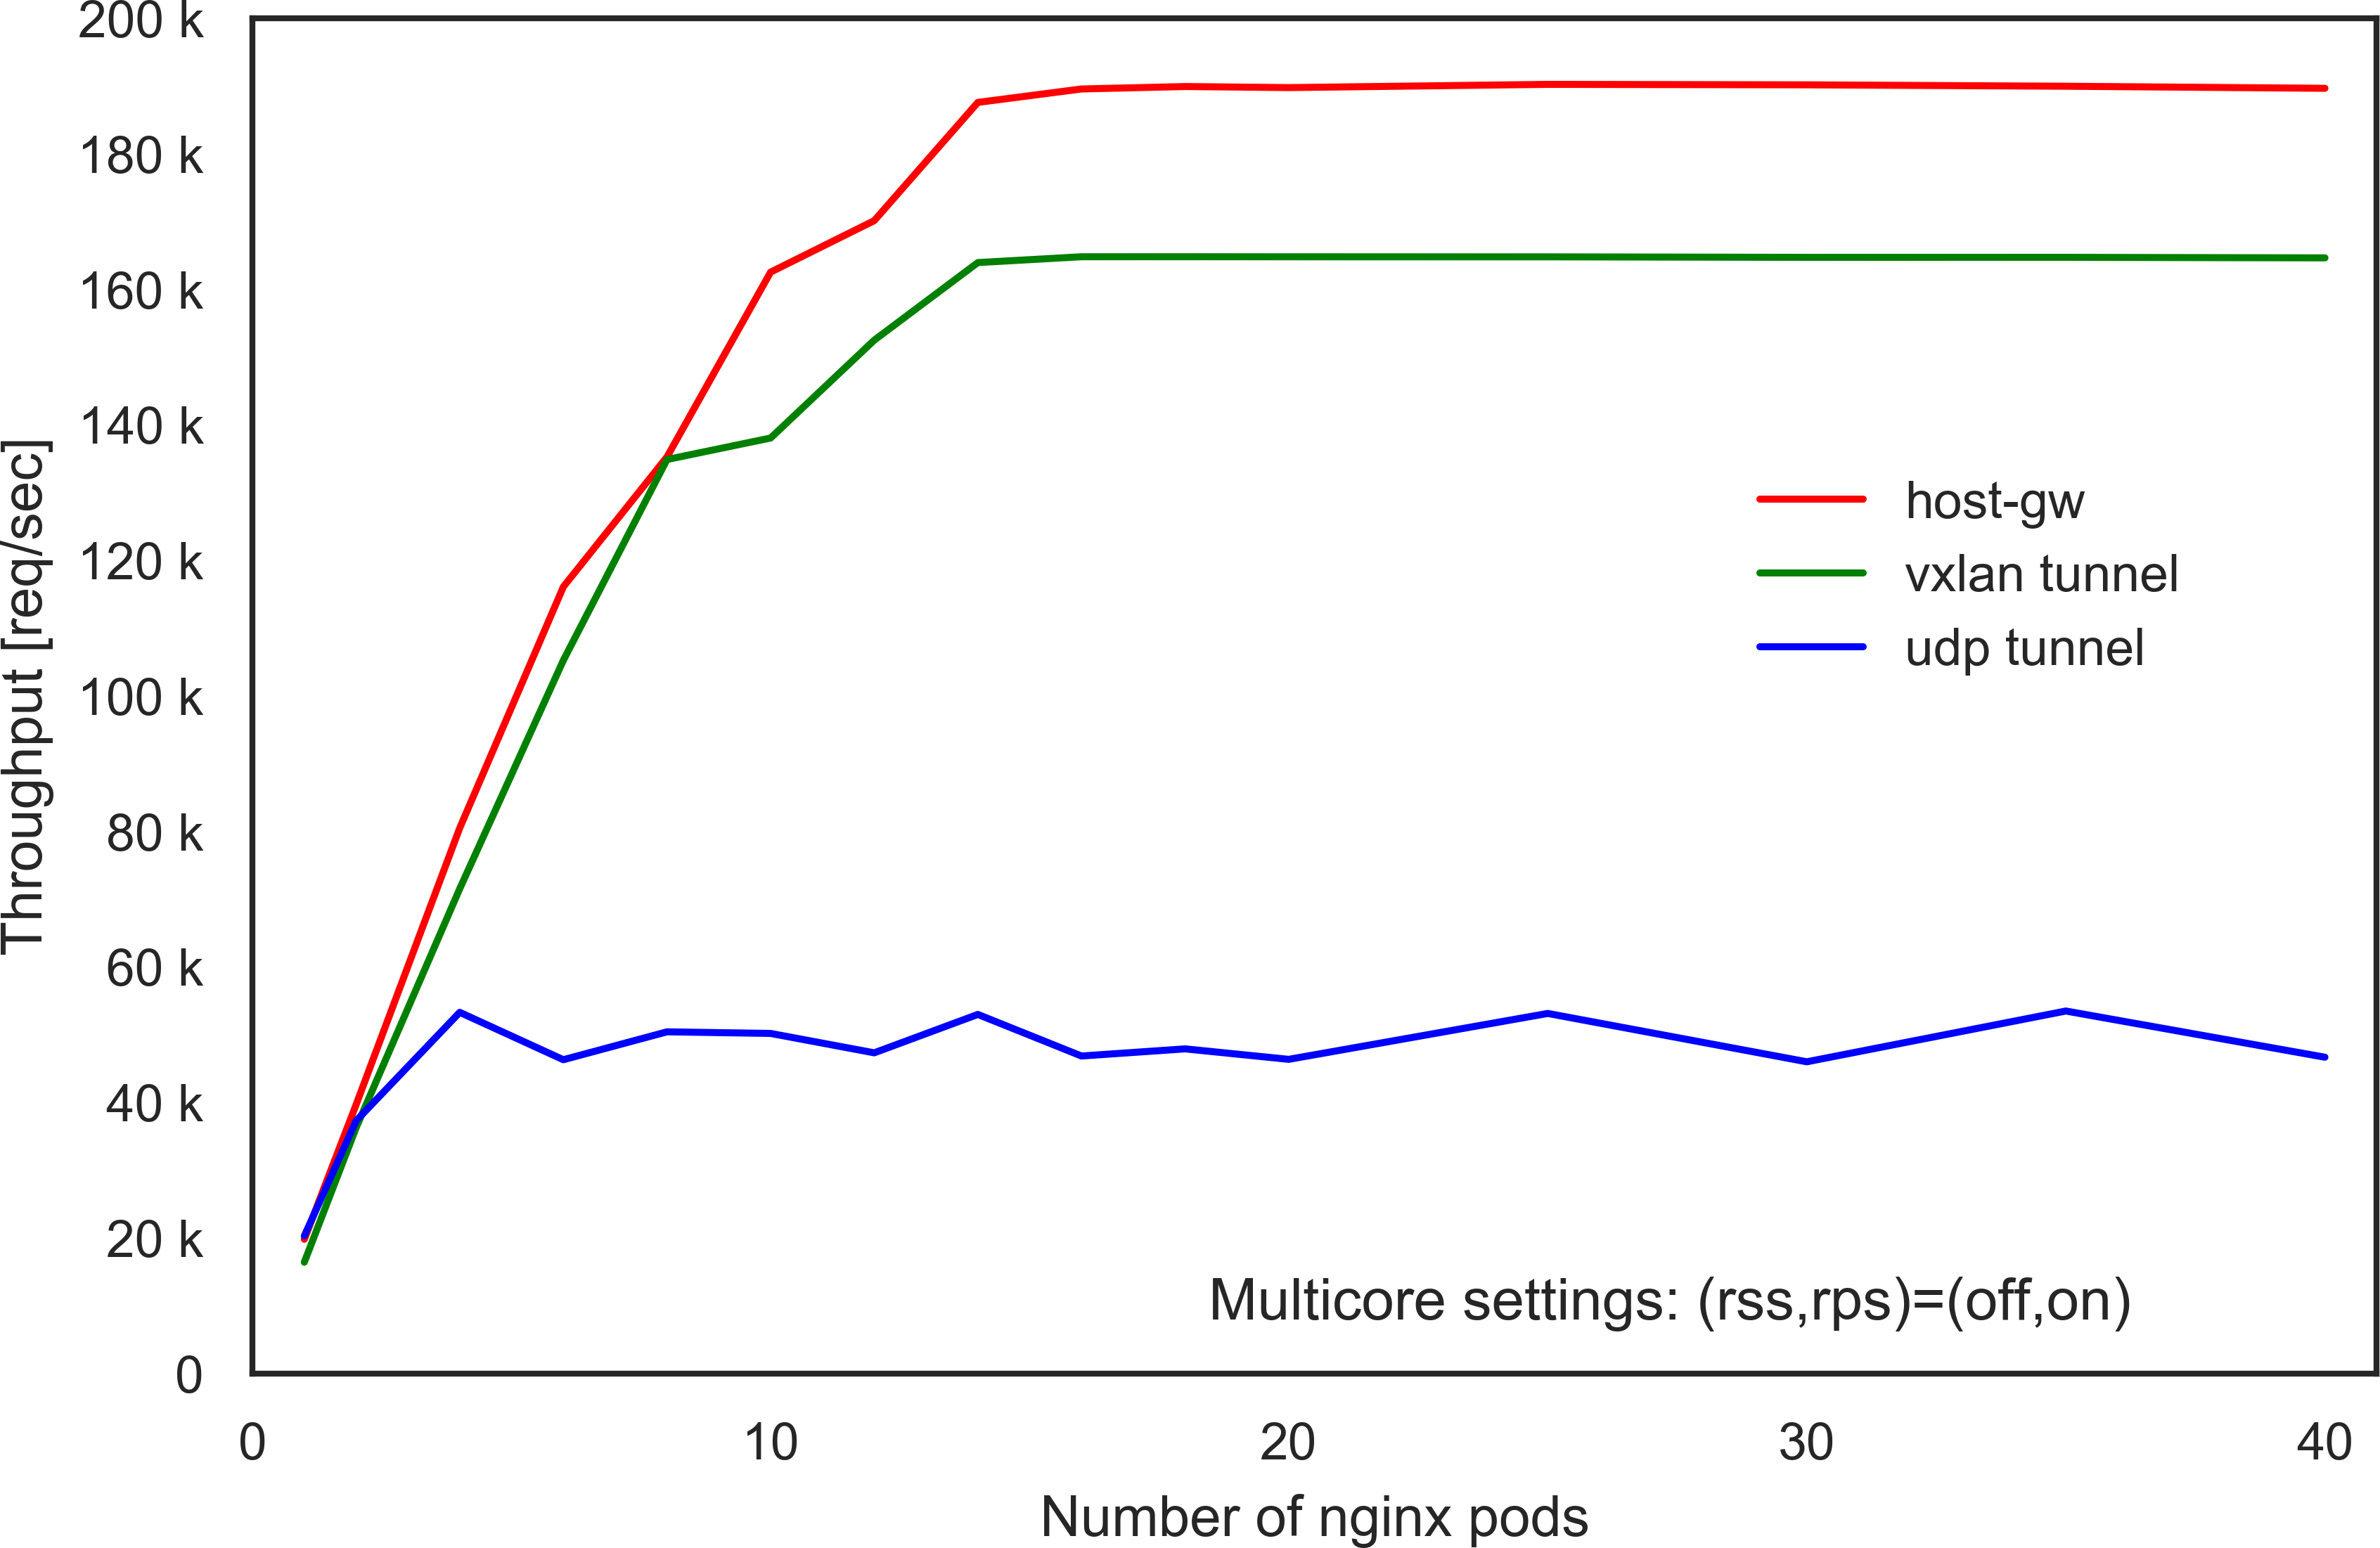
\includegraphics[width=0.75\columnwidth]{Figs/iptables_flannel_mode}

  \par\bigskip
  \centering
  \begin{minipage}{0.9\columnwidth}
    \caption[Effect of flannel backend modes on iptables DNAT throughput]{
      Effect of flannel backend modes on iptables DNAT throughput.
      the host-gw mode shows the highest performance level, followed by the vxlan mode.
      The udp mode shows significantly lower performances levels.
    }
    \label{fig:iptables_flannel_mode}
  \end{minipage}
\end{figure}

\FloatBarrier

\subsubsection{Comparison of different load balancer}

\begin{figure}[h]
  \centering
  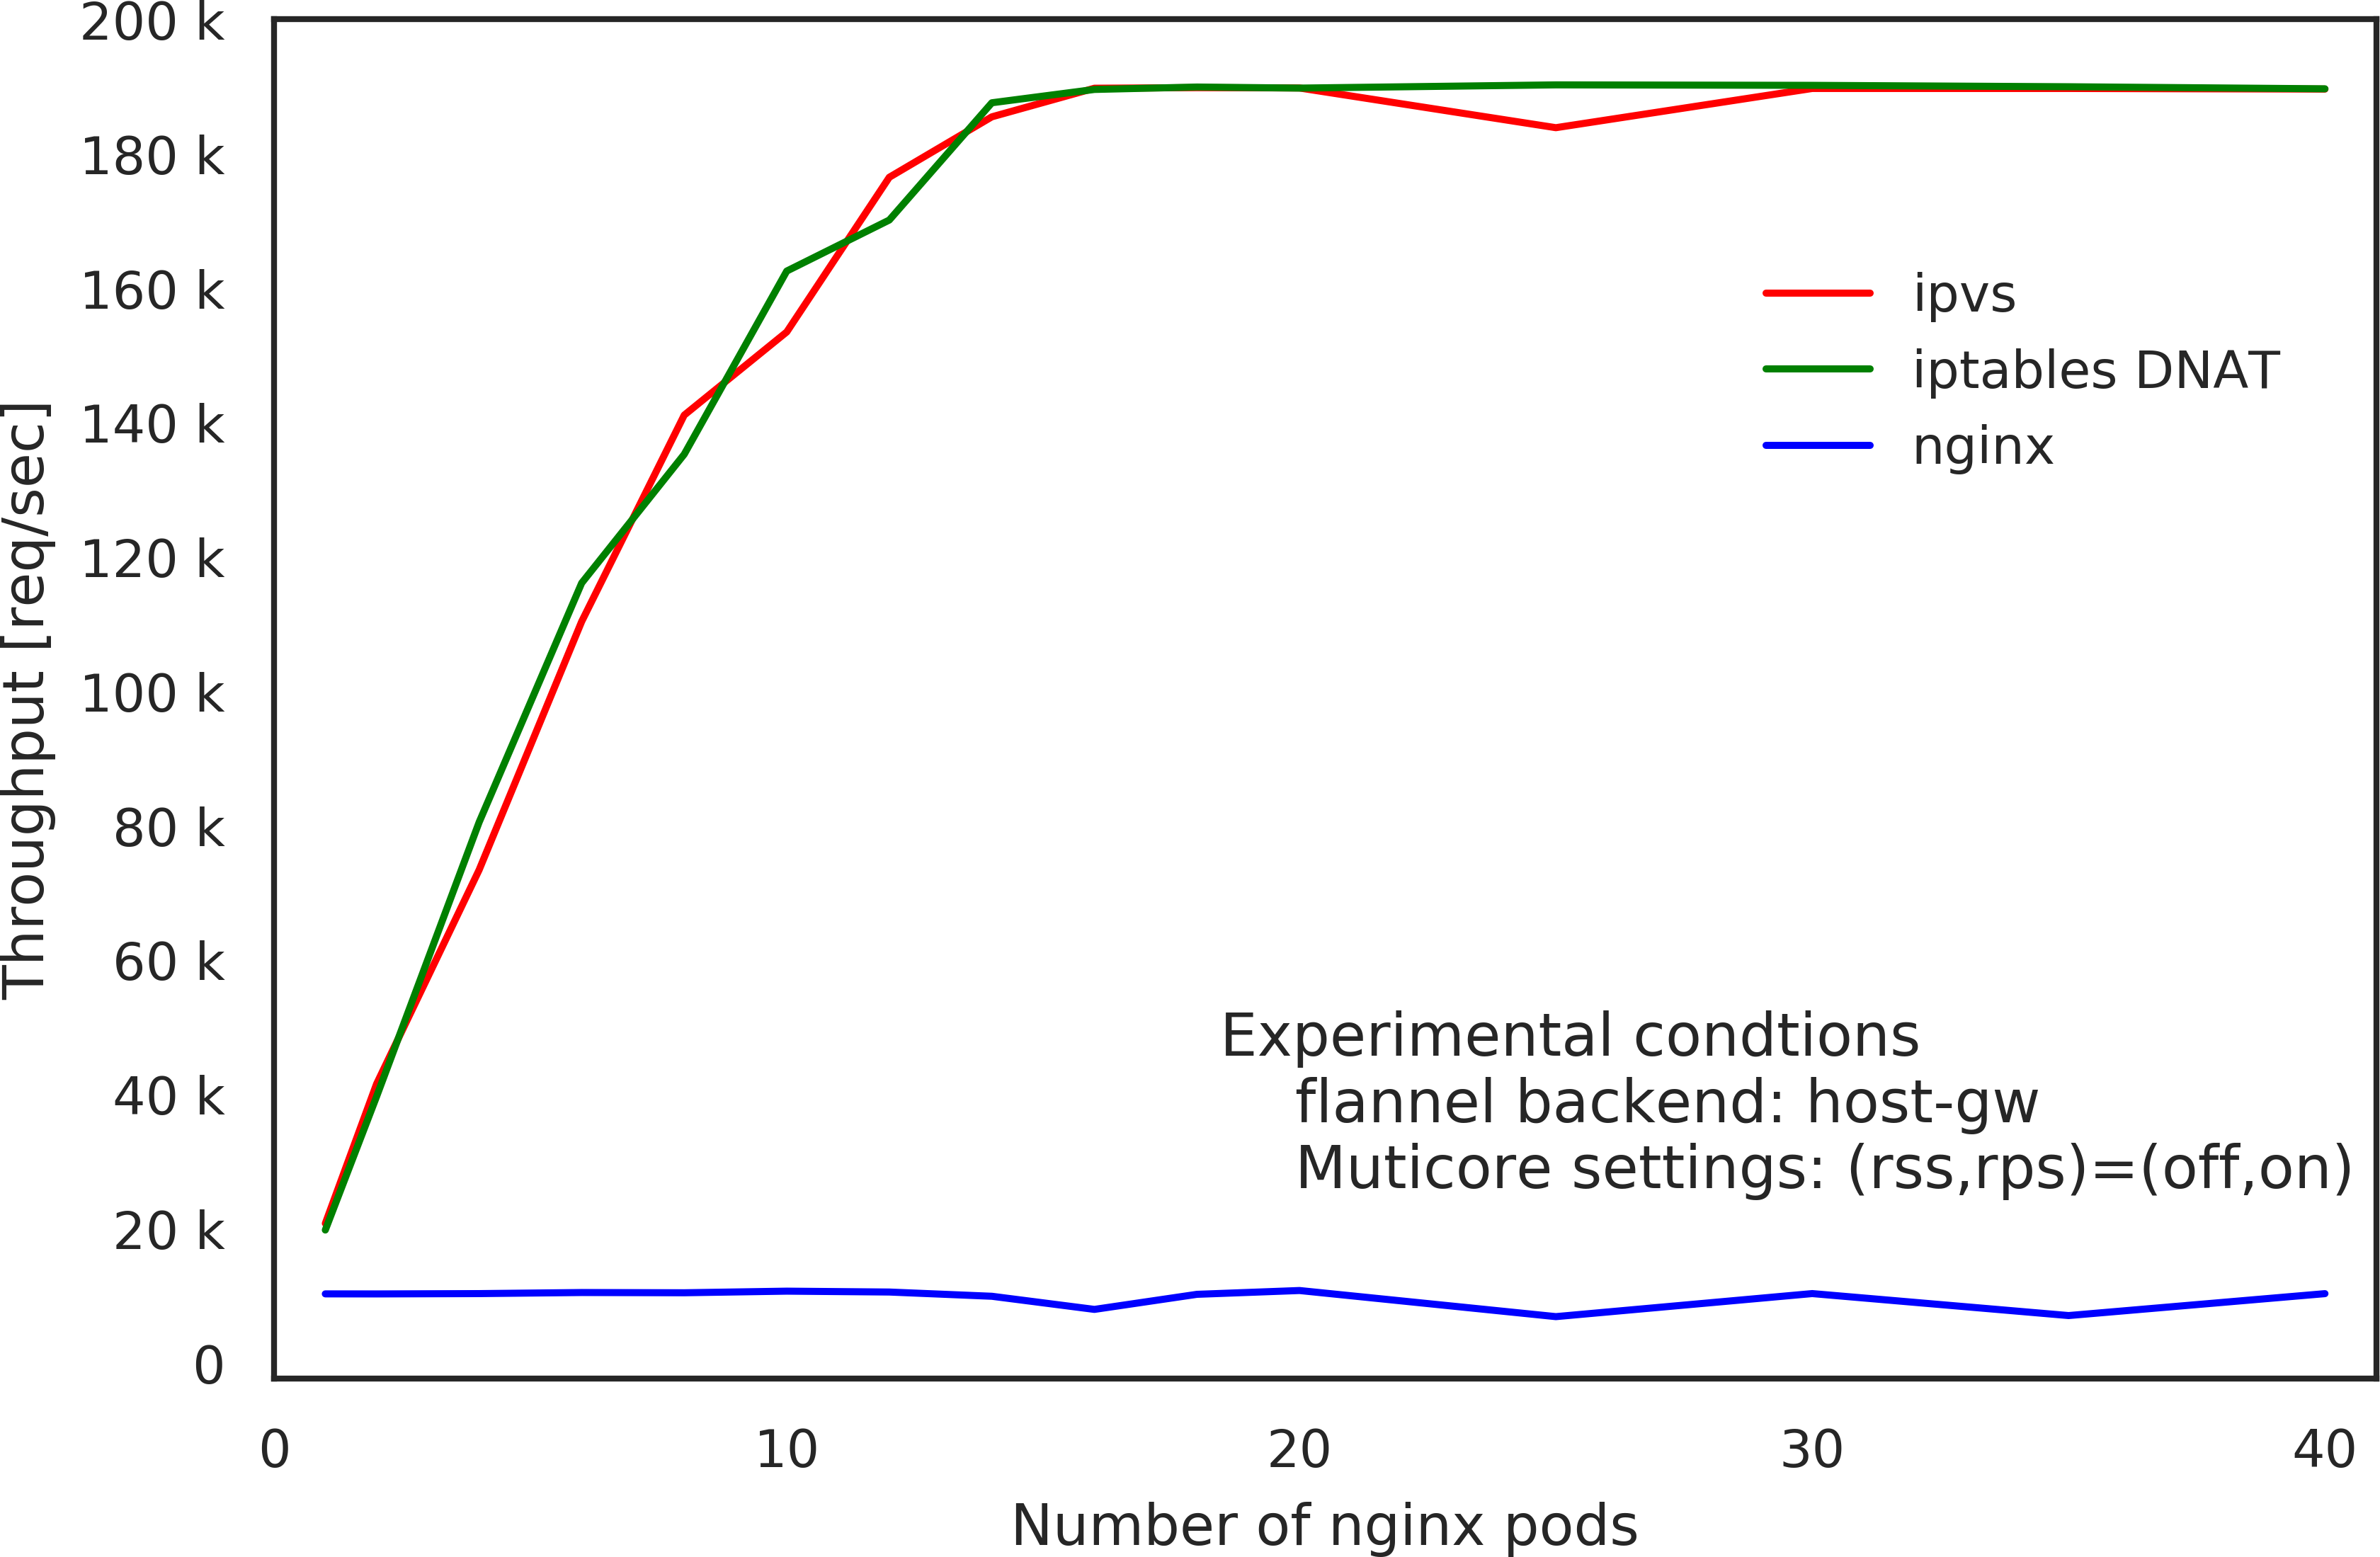
\includegraphics[width=0.75\columnwidth]{Figs/ipvs-iptables-nginx}
  \par\bigskip
  \centering
  \begin{minipage}{0.9\columnwidth}
    \caption[Throughput of ipvs, iptables DNAT and nginx]{
      Throughput of ipvs, iptables DNAT and nginx.
      The performance levels of ipvs and iptables DNAT are almost the same.
      The nginx as a load balancer does not perform well in the experiment.
    }
    \label{fig:ipvs-iptables-nginx}
  \end{minipage}
\end{figure}

\interfootnotelinepenalty=10000

Figure~\ref{fig:ipvs-iptables-nginx} presents the throughput results of the different load balancers.
The performance levels of ipvs, iptables DNAT and nginx as the load balancers are compared.
The throughput of the ipvs and iptables DNAT increases almost linearly as the number of nginx pods(web servers) increase from 1 to around 14, and then it saturates.
The proposed ipvs load balancer exhibits almost equivalent performance levels as the iptables DNAT as a load balancer.

The saturated throughput indicates the maximum performance level of the load balancer, which could be determined either by network bandwidth between the benchmark client machine and the load balancer node, or CPU performance levels of these machines.
%
In this specific experiment, the performance level was limited by the 1 Gbps bandwidth of the network
\footnote{
All of the nodes use a single interface for communication. 
At the load balancer node, the bandwidth for each direction of Full duplex Ethernet is consumed by the sum of request and response packets.
}, 
which is revealed by packet level analysis using tcpdump\cite{takahashi2018portable}.
%
On average the data size of each request and the corresponding response was about 636 [byte/req] in total, including TCP/IP headers, Ethernet header, and inter-frame gaps.
Multiplying that with 190K [req/sec] and 8 [bit/byte] will result in 966.72 Mbps.
Therefore the throughput of about 190K [req/sec] is a reasonable number as the maximum performance level in 1Gbps network environment.

While nginx did not show any benefit as the load balancer, the performance of the ipvs load balancer container showed equivalent performance level as iptables DNAT.
This means that the proposed ipvs container load balancer is at least as good as the internal load balancer for Kubernetes in the 1 Gbps network.

\begin{figure}[h]
  \centering
  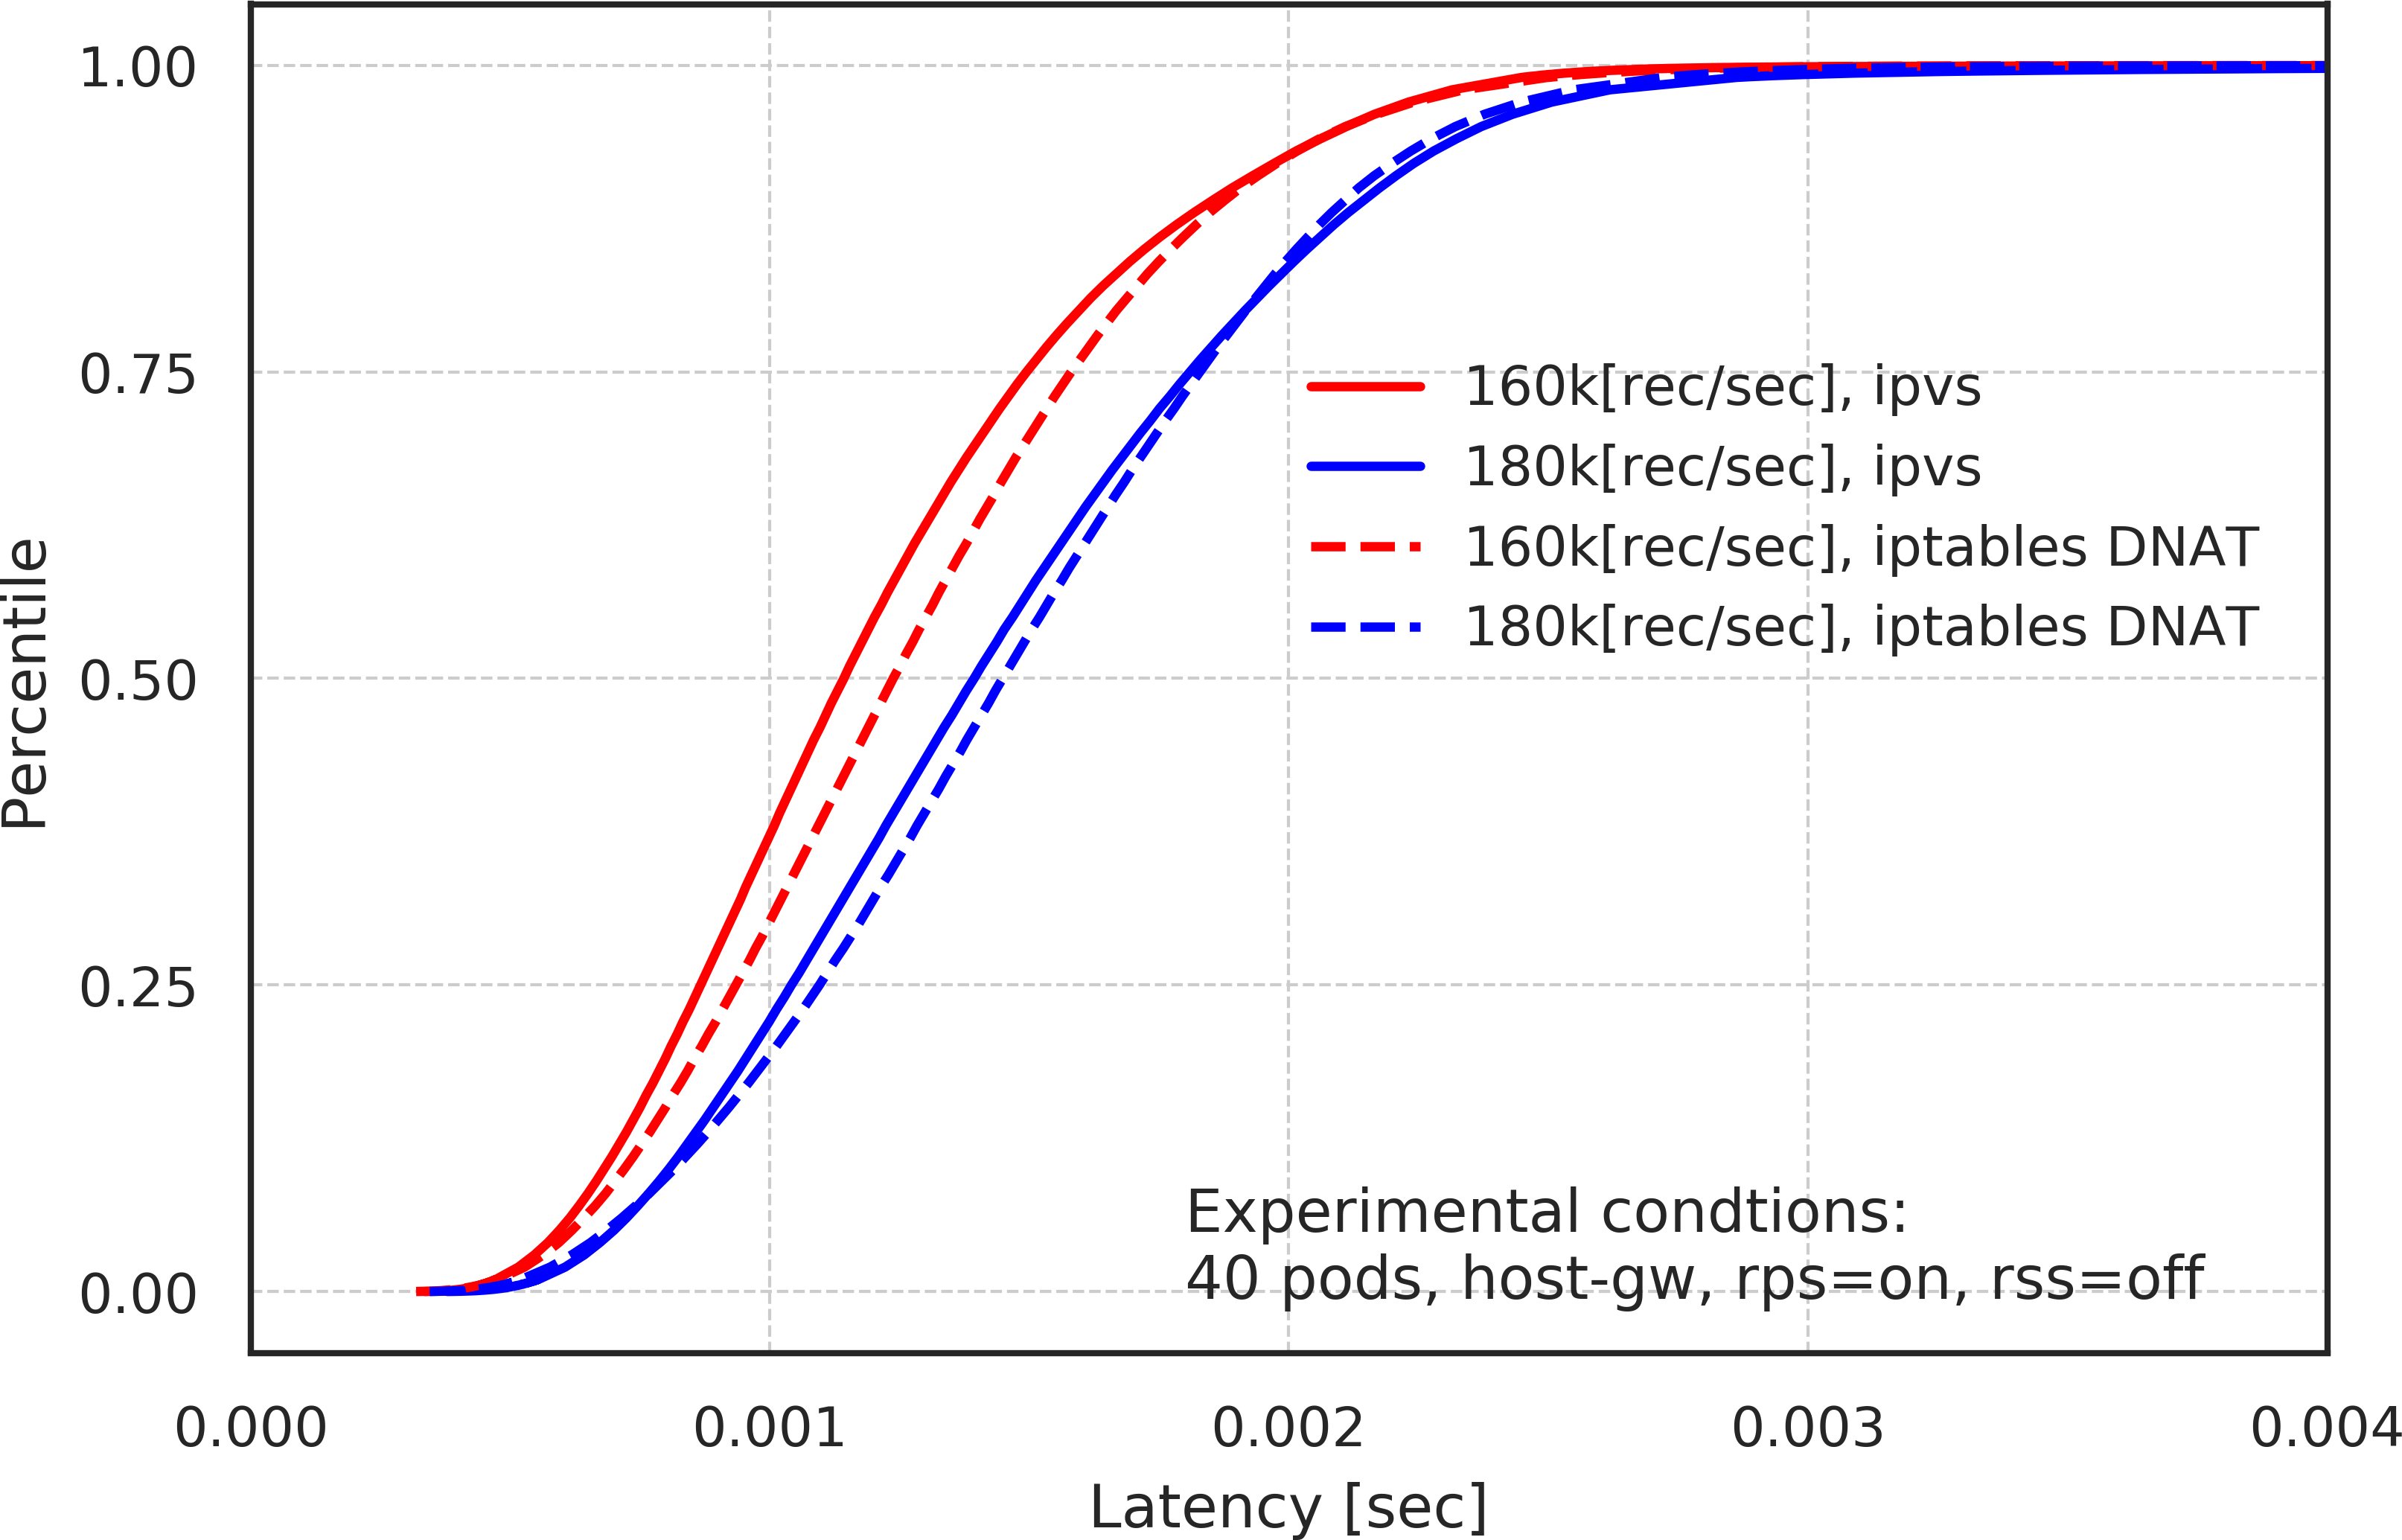
\includegraphics[width=0.75\columnwidth]{Figs/latency_cdf_rps_40pods}
  \par\bigskip
  \centering
  \begin{minipage}{0.9\columnwidth}
    \caption[Latency for ipvs and iptables DNAT]{
      Latency for ipvs and iptables DNAT.
      Cumulative Distribution Function(CDF) of the latency for ipvs and iptables DNAT are compared, at the two constant loads, 160K[req/sec] and 180K[req/sec] .
      Smaller latencies are observed for ipvs.
}
    \label{fig:latency_cdf_rps_40pods}
  \end{minipage}
\end{figure}

Figure~\ref{fig:latency_cdf_rps_40pods} compares Cumulative Distribution Function(CDF) of the load balancer latency at the two constant loads, 160K[req/sec] and 180K[req/sec] for ipvs and iptables DNAT.
It is seen that the latencies are a little bit smaller for ipvs.
For example, the median values at 160K[req/sec] load for ipvs and iptables DNAT are, 1.14 msec and 1.24 msec, respectively.
Also, at 160K[req/sec], they are 1.39 msec and 1.45 msec, respectively.
%
While these may be considered a subtle difference, however, this indicates that proposed load balancer is at least as good as iptables DNAT.

%% Fig.~\ref{fig:cpu_usage} compares the CPU usage for the proposed ipvs load balancer in container and iptables DNAT at the time of the throughput measurement in the on-premise data center.
%% Since the CPU usage was higher for the ipvs in a container, the proposed load balancer may be less efficient compared with the iptables DNAT.
%% However, since single hardware can accommodate 1 Gbps traffic with CPU usage of about 60\%, the authors regard this as a tolerable overhead.

%% The author tries to improve the efficiency of the proposed load balancer by developing a software load balancer using eXpress data path(XDP) technology\cite{hoiland2018express} later and thereby improving the performance levels of the portable load balancer.

%% \begin{figure}[h]
%%   \centering
%%   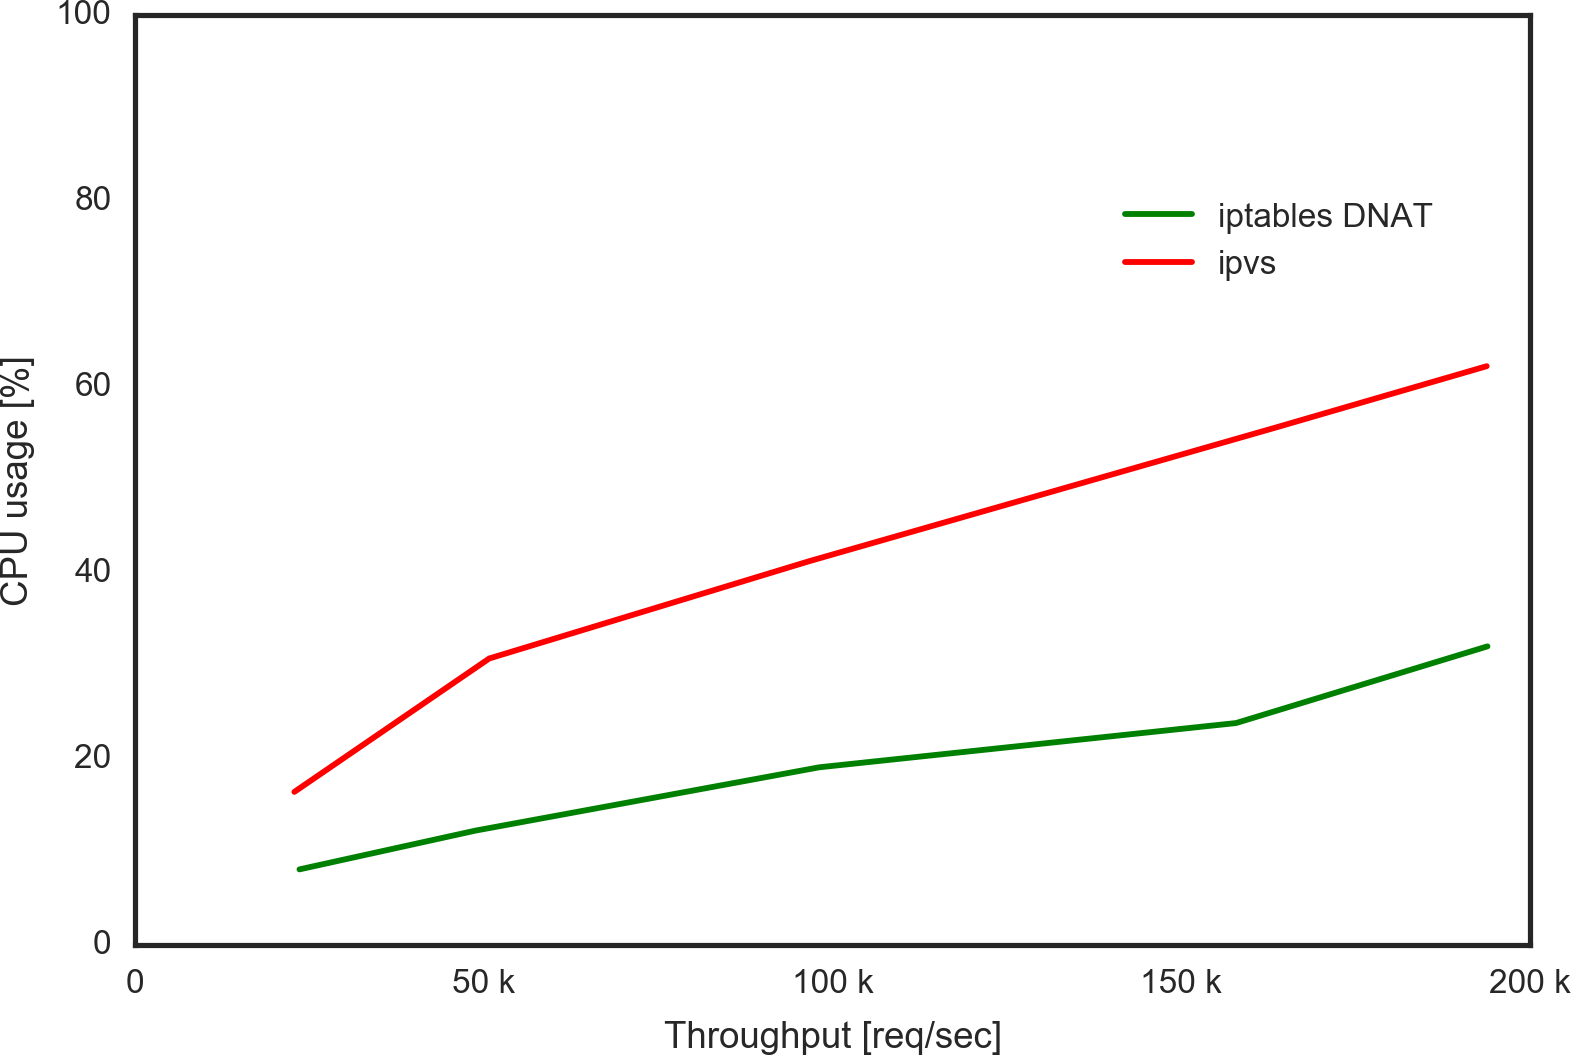
\includegraphics[width=0.75\columnwidth]{Figs/cpu_usage}
%%   \par\bigskip
%%   \centering
%%   \begin{minipage}{0.9\columnwidth}
%%     \caption[CPU usage of the ipvs and iptables DNAT]{
%%       CPU usage of the ipvs and iptables DNAT.
%%       CPU usage of ipvs is higher than that of iptables DNAT.
%%     }
%%     \label{fig:cpu_usage}
%%   \end{minipage}
%% \end{figure}

\FloatBarrier

\subsubsection{L3DSR using ipvs-tun}

The performance levels of ipvs and iptables DNAT have been limited by 1 Gbps bandwidth.
This can be alleviated in the case of ipvs by using so-called Layer 3 Direct Server Return(L3DSR) setup.
Figure~\ref{fig:benchmark-schem-dsr} shows the schematic diagram illustrating the packet flow of the L3DSR experiment.
The red arrows indicate the route HTTP request packets follow and the blue arrows indicate the route response packets follow.
Since the response packets directly return to the client, the load balancer is expected to perform better.

The ipvs has a mode called ipvs-tun.
When the ipvs-tun send out the packets to real servers, it encapsulates the original packet in ipip tunneling packet that is destined to real servers.
The real server receives the packet on a tunl0 device and decapsulates the ipip packet, revealing the original packet.
Since the source IP address of the original packet is maintained, the returning packets are sent directly toward the benchmark client.
In this scheme, the returning packets do not consume the bandwidth nor the CPU power of the load balancer node.
Since iptables DNAT does not have the functions that enable L3DSR settings, this is one of the benefits available only for the proposed load balancer.

\begin{figure}[h]
  \centering
  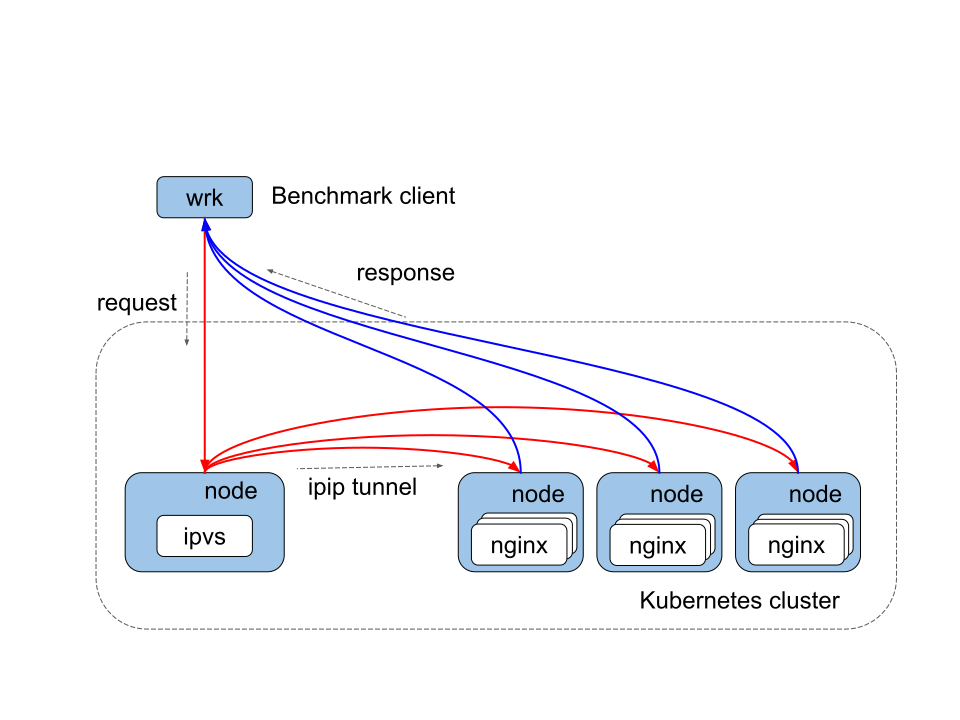
\includegraphics[width=0.8\columnwidth]{Figs/benchmark-schem-dsr}
  \par\bigskip
  \centering
  \begin{minipage}{0.9\columnwidth}
    \caption[Experimental setup for L3DSR throughput measurement]{
      Experimental setup for L3DSR throughput measurement.
      The red arrows indicate the route HTTP request packets follow and the blue arrows indicate the route response packets follow.
      Since the response packets directly return to the client, the load balance is expected to perform better.
    }
    \label{fig:benchmark-schem-dsr}
  \end{minipage}
\end{figure}

\begin{figure}[h]
  \centering
  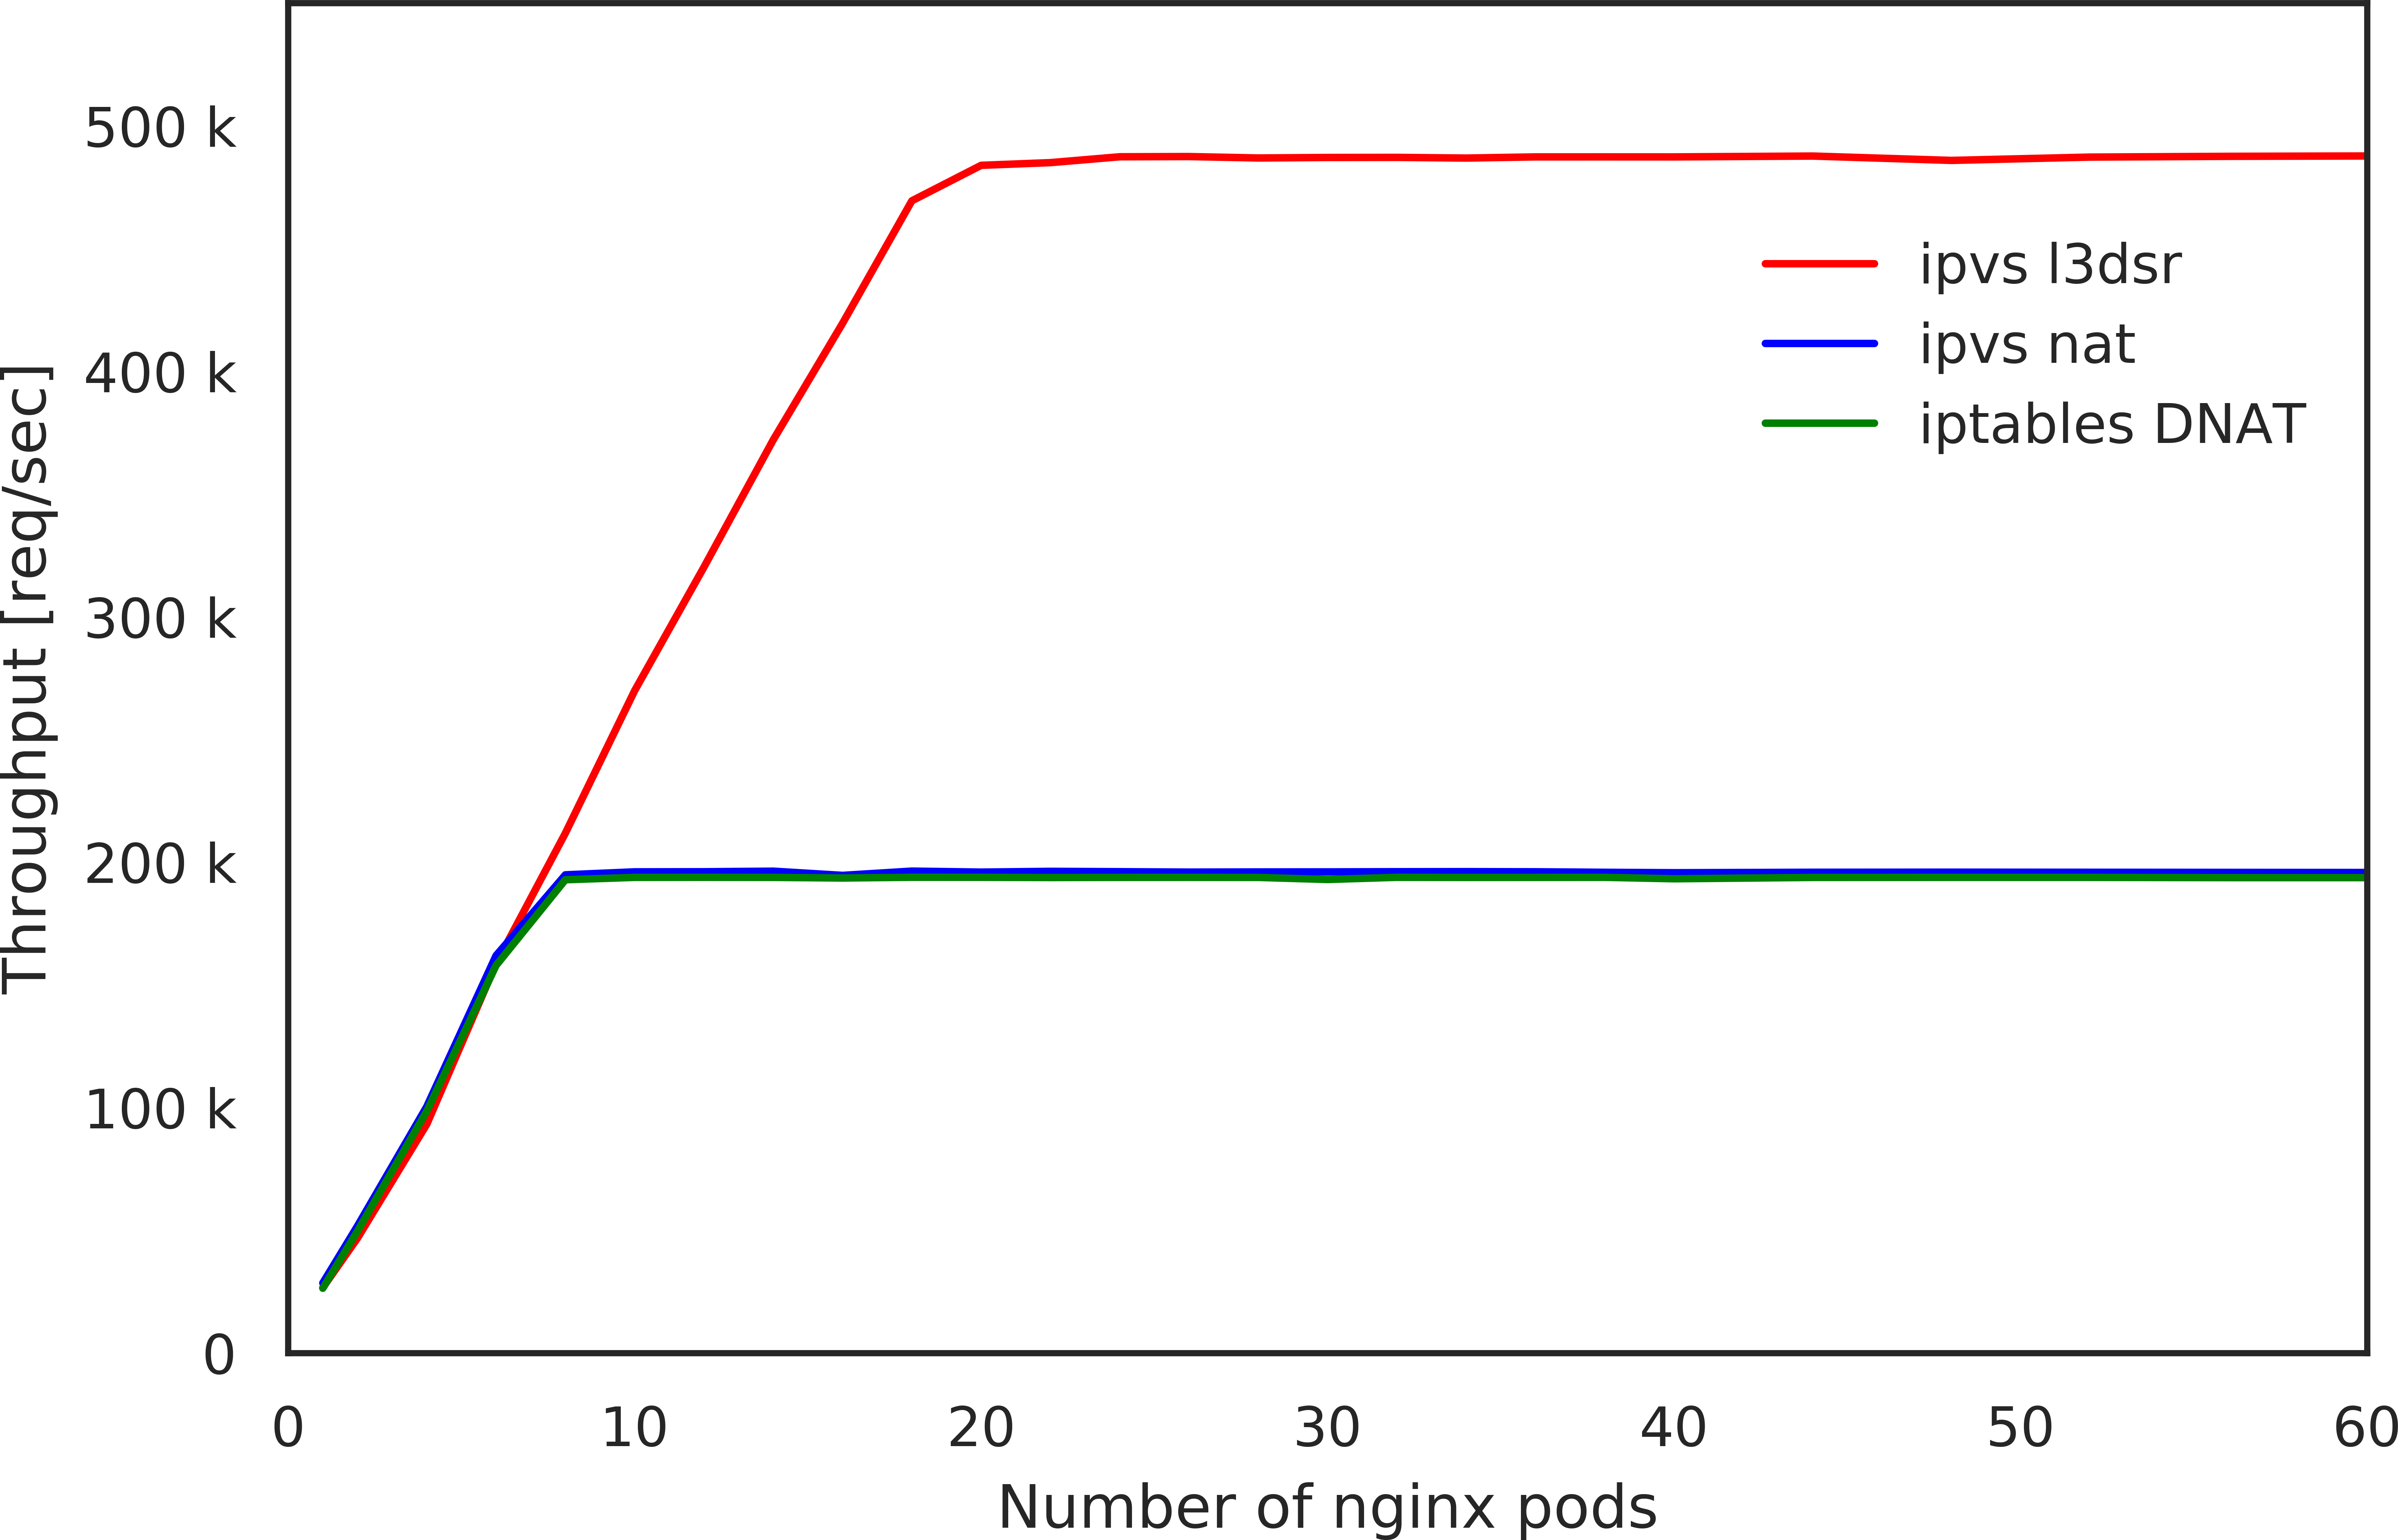
\includegraphics[width=0.75\columnwidth]{Figs/ipvs_l3dsr_1g.png}
  \par\bigskip
  \centering
  \begin{minipage}{0.9\columnwidth}
    \caption[Throughput of L3DSR using ipvs-tun.]{
      Throughput of L3DSR using ipvs-tun.
      The throughput of ipvs-tun is 1.5 times higher than those of conventional ipvs and iptables DNAT.
    }
    \label{fig:ipvs_l3dsr_1g.png}
  \end{minipage}
\end{figure}

The author carried out throughput measurement using the experimental setup shown in Figure~\ref{fig:benchmark-schem-dsr}.
Figure~\ref{fig:ipvs_l3dsr_1g.png} compares the throughput of the ipvs-tun, conventional ipvs and iptables DNAT.
As can be seen in the figure, while the performance levels for ipvs and iptables DNAT exactly match, the performance level of ipvs-tun is much higher than those.
For example, the throughput of ipvs-tun is about 1.5 times higher than those of conventional ipvs and iptables DNAT.
\footnote{The limit is due to the bandwidth of benchmark client's NIC.
Multipling 290K [req/sec] with the response packet size 450[byte/req](Appendix~\ref{appendix:performance_limit}) and 8 [bit/byte] results in 972M [bit/sec] . }
\mytodo[inline]{do that packet analysis again}

%\mytodo[inline]{Add tunneling setup needed on web container for L3DSR, if there is enough time. }

%% The author summarises this section as follows;
%% In experiments in 1Gbps network, the proposed load balancer, i.e., ipvs in container showed equivalent performance level as the iptables DNAT as a load balancer.
%% The efficiency of the ipvs may be inferior to that of iptables DNAT.
%% By using the ipvs-tun (L3DSR mode), the throughput of the proposed load balancer improved 1.5 times.

\FloatBarrier

\section{Cloud experiment}

The throughput measurements were also carried in GCP and AWS to show the containerized ipvs load balancer is runnable even in the cloud environment.
The specifications of virtual machines used for the experiment in both environment are summarized in Table~\ref{fig:gcp_machine_spec} and Table~\ref{fig:aws_machine_spec}.
In the cases of cloud environments, it is easy to change the machine specifications, especially CPU counts.
Therefore, the author measured throughput with several conditions of them.
In the case of GCP, custom instance with 32Gbyte memory and with 8, 16, and 32 CPU are used.
And in the case of AWS instance type of c4.2xlarge, c4.4xlarge, and c4.8xlarge are used.
The vxlan mode of the flannel is used for the overlay network in both of the cloud environment.
As for multicore packet processing, different settings depending on the number of prepared queues for VMs are used. 
The setting \enquote{(RSS, RPS) = (on, off)} is used in GCP and the setting \enquote{(RSS, RPS) = (off, on)} is used in AWS.

{
\setlength{\tabcolsep}{3em}
\renewcommand{\arraystretch}{1.1}

\begin{table}[h]
  \centering
  \begin{tabular}{ll}
    \hline 
    \multicolumn{2}{l}{[GCP VM Instance Specification for Client and Web Server Nodes ]}   \\
    & Instance type: custom instance \\
    & CPU: Xeon 2.2GHz, 16 cpus \hspace{2cm} \\
    & Memory: 16GB \\
    & NIC: virtio\_net /w 16 rx-queues \\
    & (Node x 6, Client x 1) \\
    & \\
    \multicolumn{2}{l}{[GCP VM Instance Specification for Load balancer Node ]}   \\
    & Instance type: custom instance \\
    & CPU: Xeon 2.2GHz, 8, 16, 32 cpus \hspace{2cm} \\
    & Memory: 16GB \\
    & NIC: virtio\_net /w 8, 16, 32 rx-queues \\
    & (Load balancer x 1) \\
    \hline
  \end{tabular}
  \par\bigskip
  \centering
  \begin{minipage}{0.9\columnwidth}
    \caption[Virtual Machine specifications in GCP experiment]{
Virtual Machine specifications in GCP experiment.
The author measured throughputs using load balancer nodes with 8 CPUs, 16 CPUs, and 32 cups.
The number of rx-queues of each node was 8, 16 and 32, respectively.
Since the same number of rx-queues as the number CPU is prepared, the setting with \enquote{(rss, rps) = (on, off)} is used.
    }
    \label{fig:gcp_machine_spec}
  \end{minipage}
\end{table}
}

{
\setlength{\tabcolsep}{3em}
\renewcommand{\arraystretch}{1.1}

\begin{table}[h]
  \centering
  \begin{tabular}{ll}
    \hline 
    \multicolumn{2}{l}{[AWS VM Instance Specification for Client and Web Server Nodes ]}   \\
    & Instance type: m4.4xlarge \\
    & CPU: Xeon E5-2686 v4 2.30GHz, 16 cpus \\
    & Memory: 64GB \\
    & NIC: ixgbevf /w 2 rx-queues \\
    & (Node x 6, Client x 1) \\
    & \\
    \multicolumn{2}{l}{[AWS VM Instance Specification for Load balancer Node ]}   \\
    & Instance type: c4.2xlarge, c4.4xlarge, c4.8xlarge  \\
    & CPU: Xeon E5-2666 v3 2.90GHz, 8, 16, 36 cpus \\
    & Memory: 15GB, 30GB, 60GB \\
    & NIC: ixgbevf /w 2 rx-queues \\
    & (Load balancer x 1) \\
    \hline
  \end{tabular}
  \par\bigskip
  \centering
  \begin{minipage}{0.9\columnwidth}
    \caption[Virtual Machine specifications in AWS experiment]{
Virtual Machine specifications in AWS experiment.
The author measured throughputs using load balancer nodes with 8 CPUs, 16 CPUs, and 36 CPUs.
Since there are only two rx-queues, the setting with \enquote{(rss, rps) = (off, on)} is used.
    }
    \label{fig:aws_machine_spec}
  \end{minipage}
\end{table}
}


\begin{figure}[h]
  \centering
  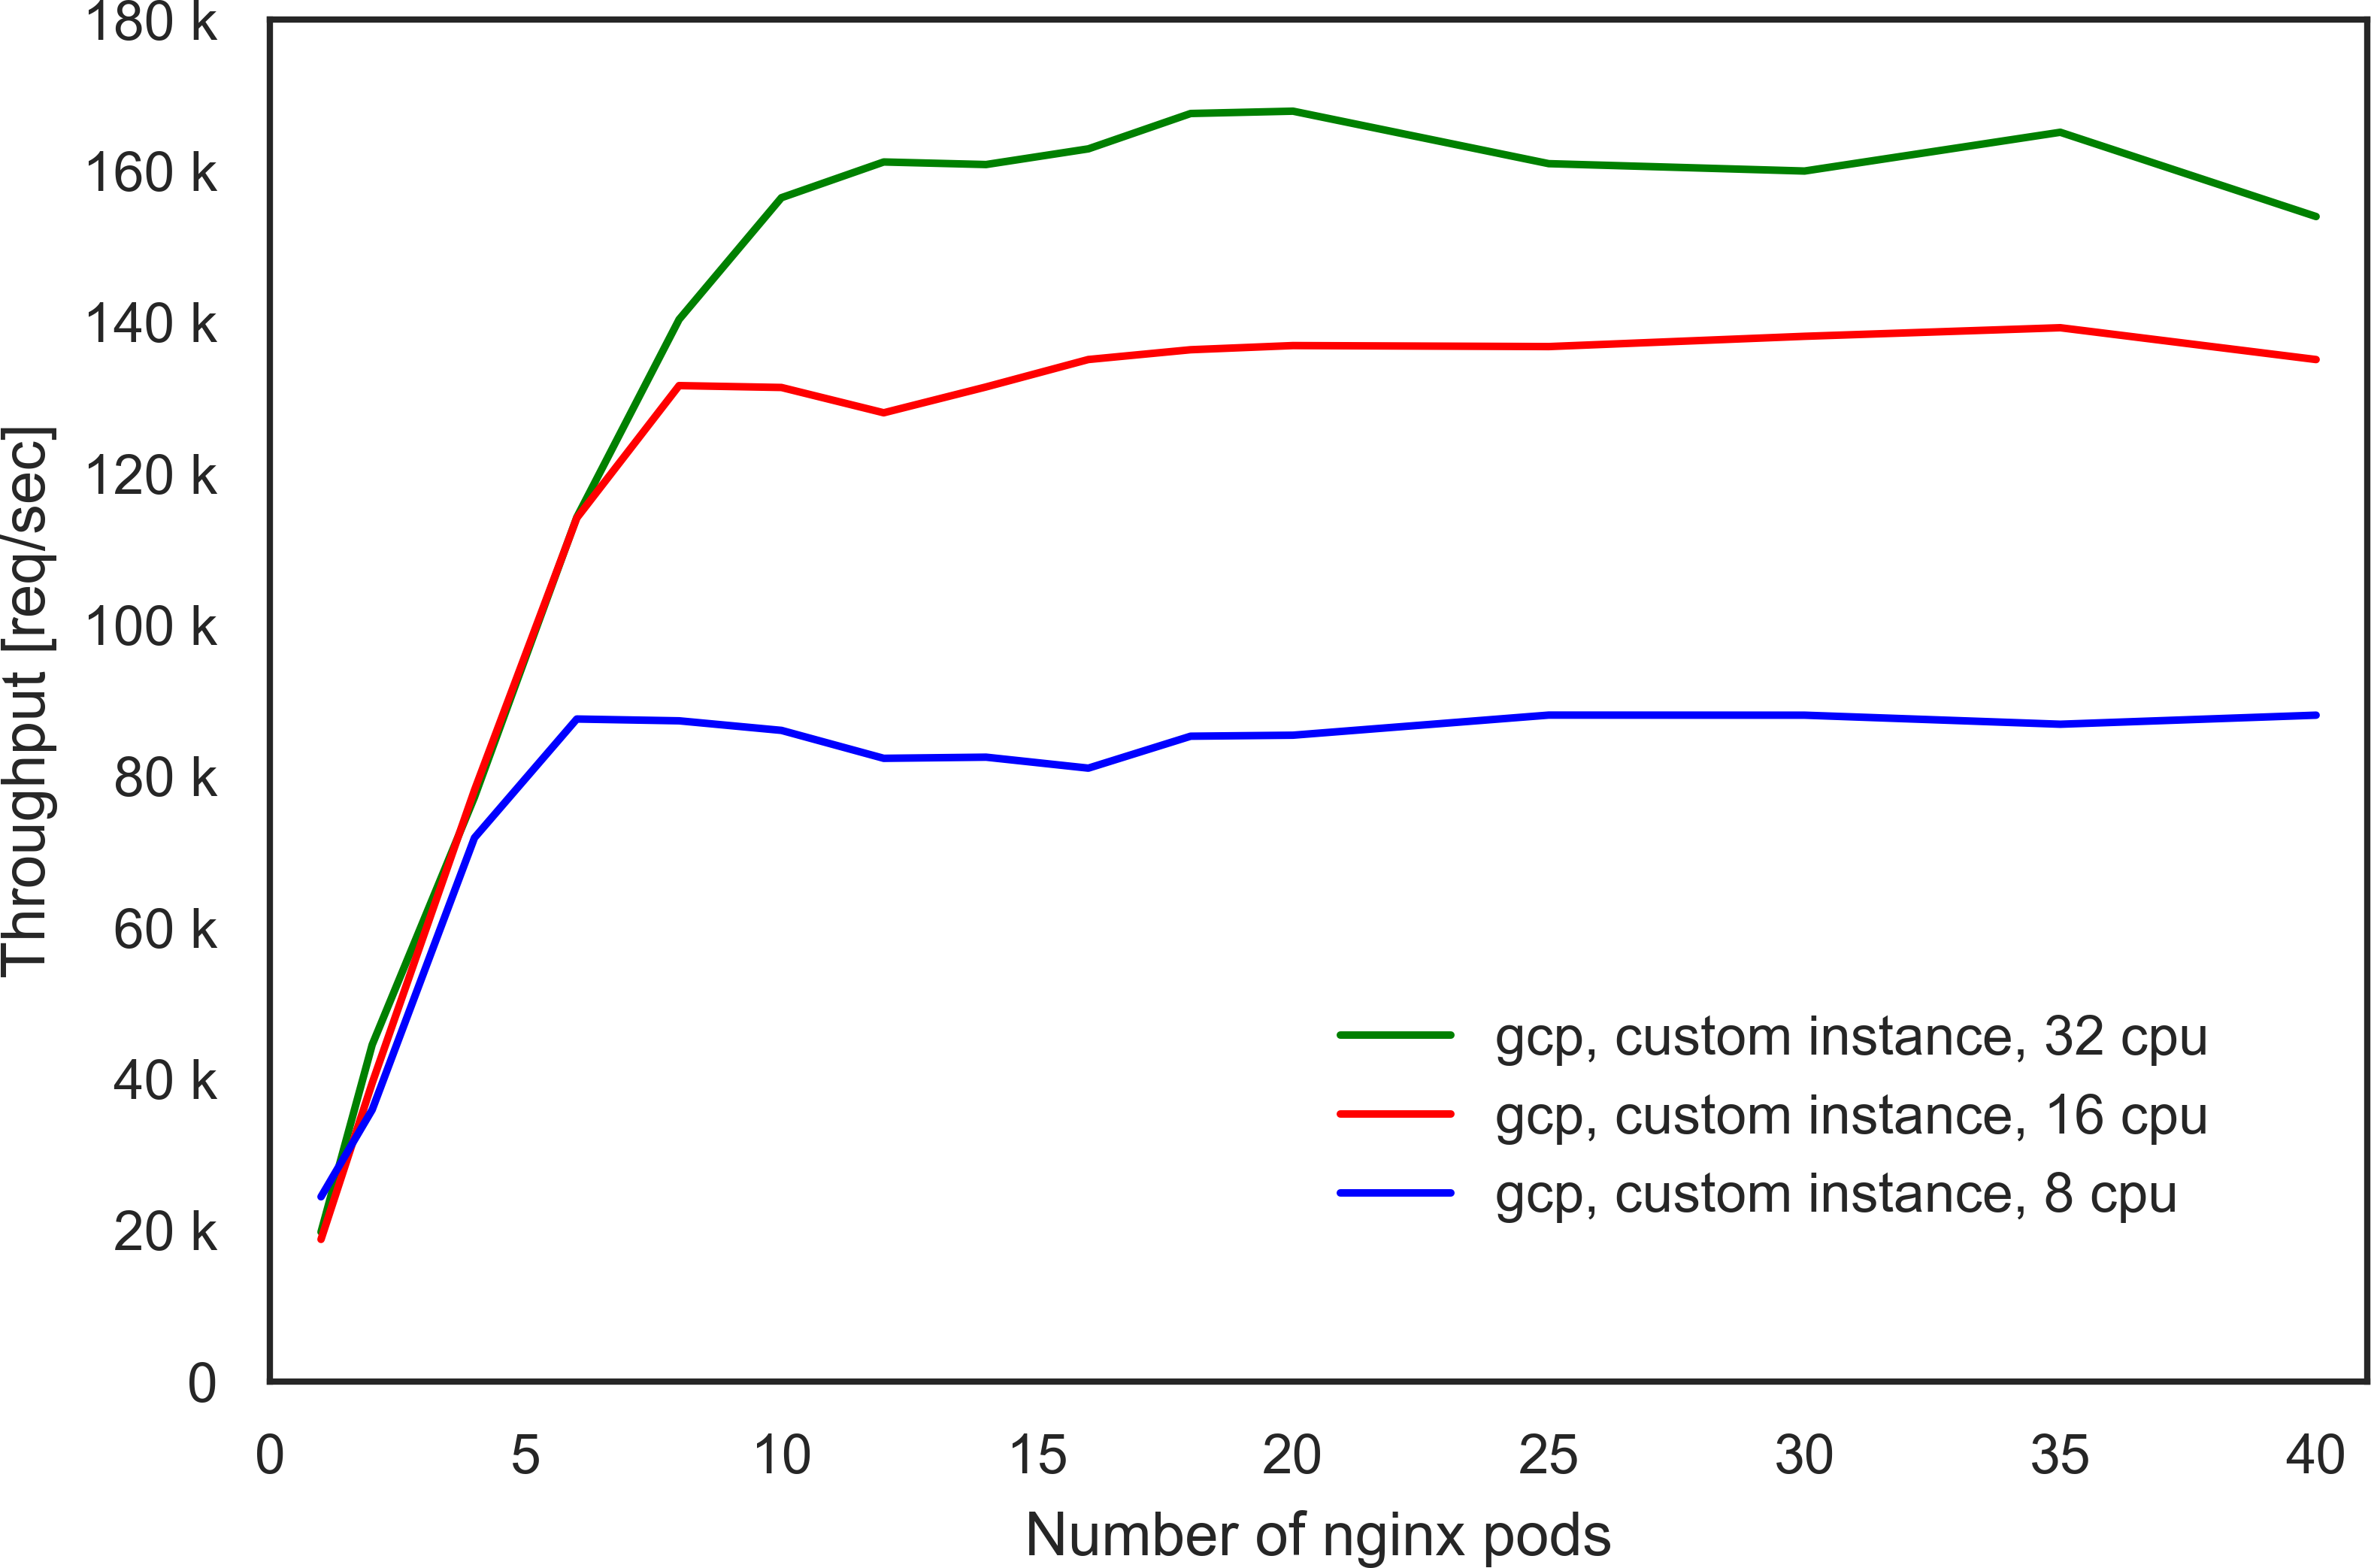
\includegraphics[width=0.75\columnwidth]{Figs/gcp_all_tp}
  \par\bigskip
  \centering
  \begin{minipage}{0.9\columnwidth}
    \caption[Throughput measurement results in GCP]{
Throughput measurement results in GCP.
The throughput increases linearly as the number of nginx {\em pod}s increases until it reaches the saturation level.
The maximum throughput is higher for instances with more virtual CPUs.
    }
    \label{fig:gcp_all_tp}
  \end{minipage}
\end{figure}


\begin{figure}[h]
  \centering
  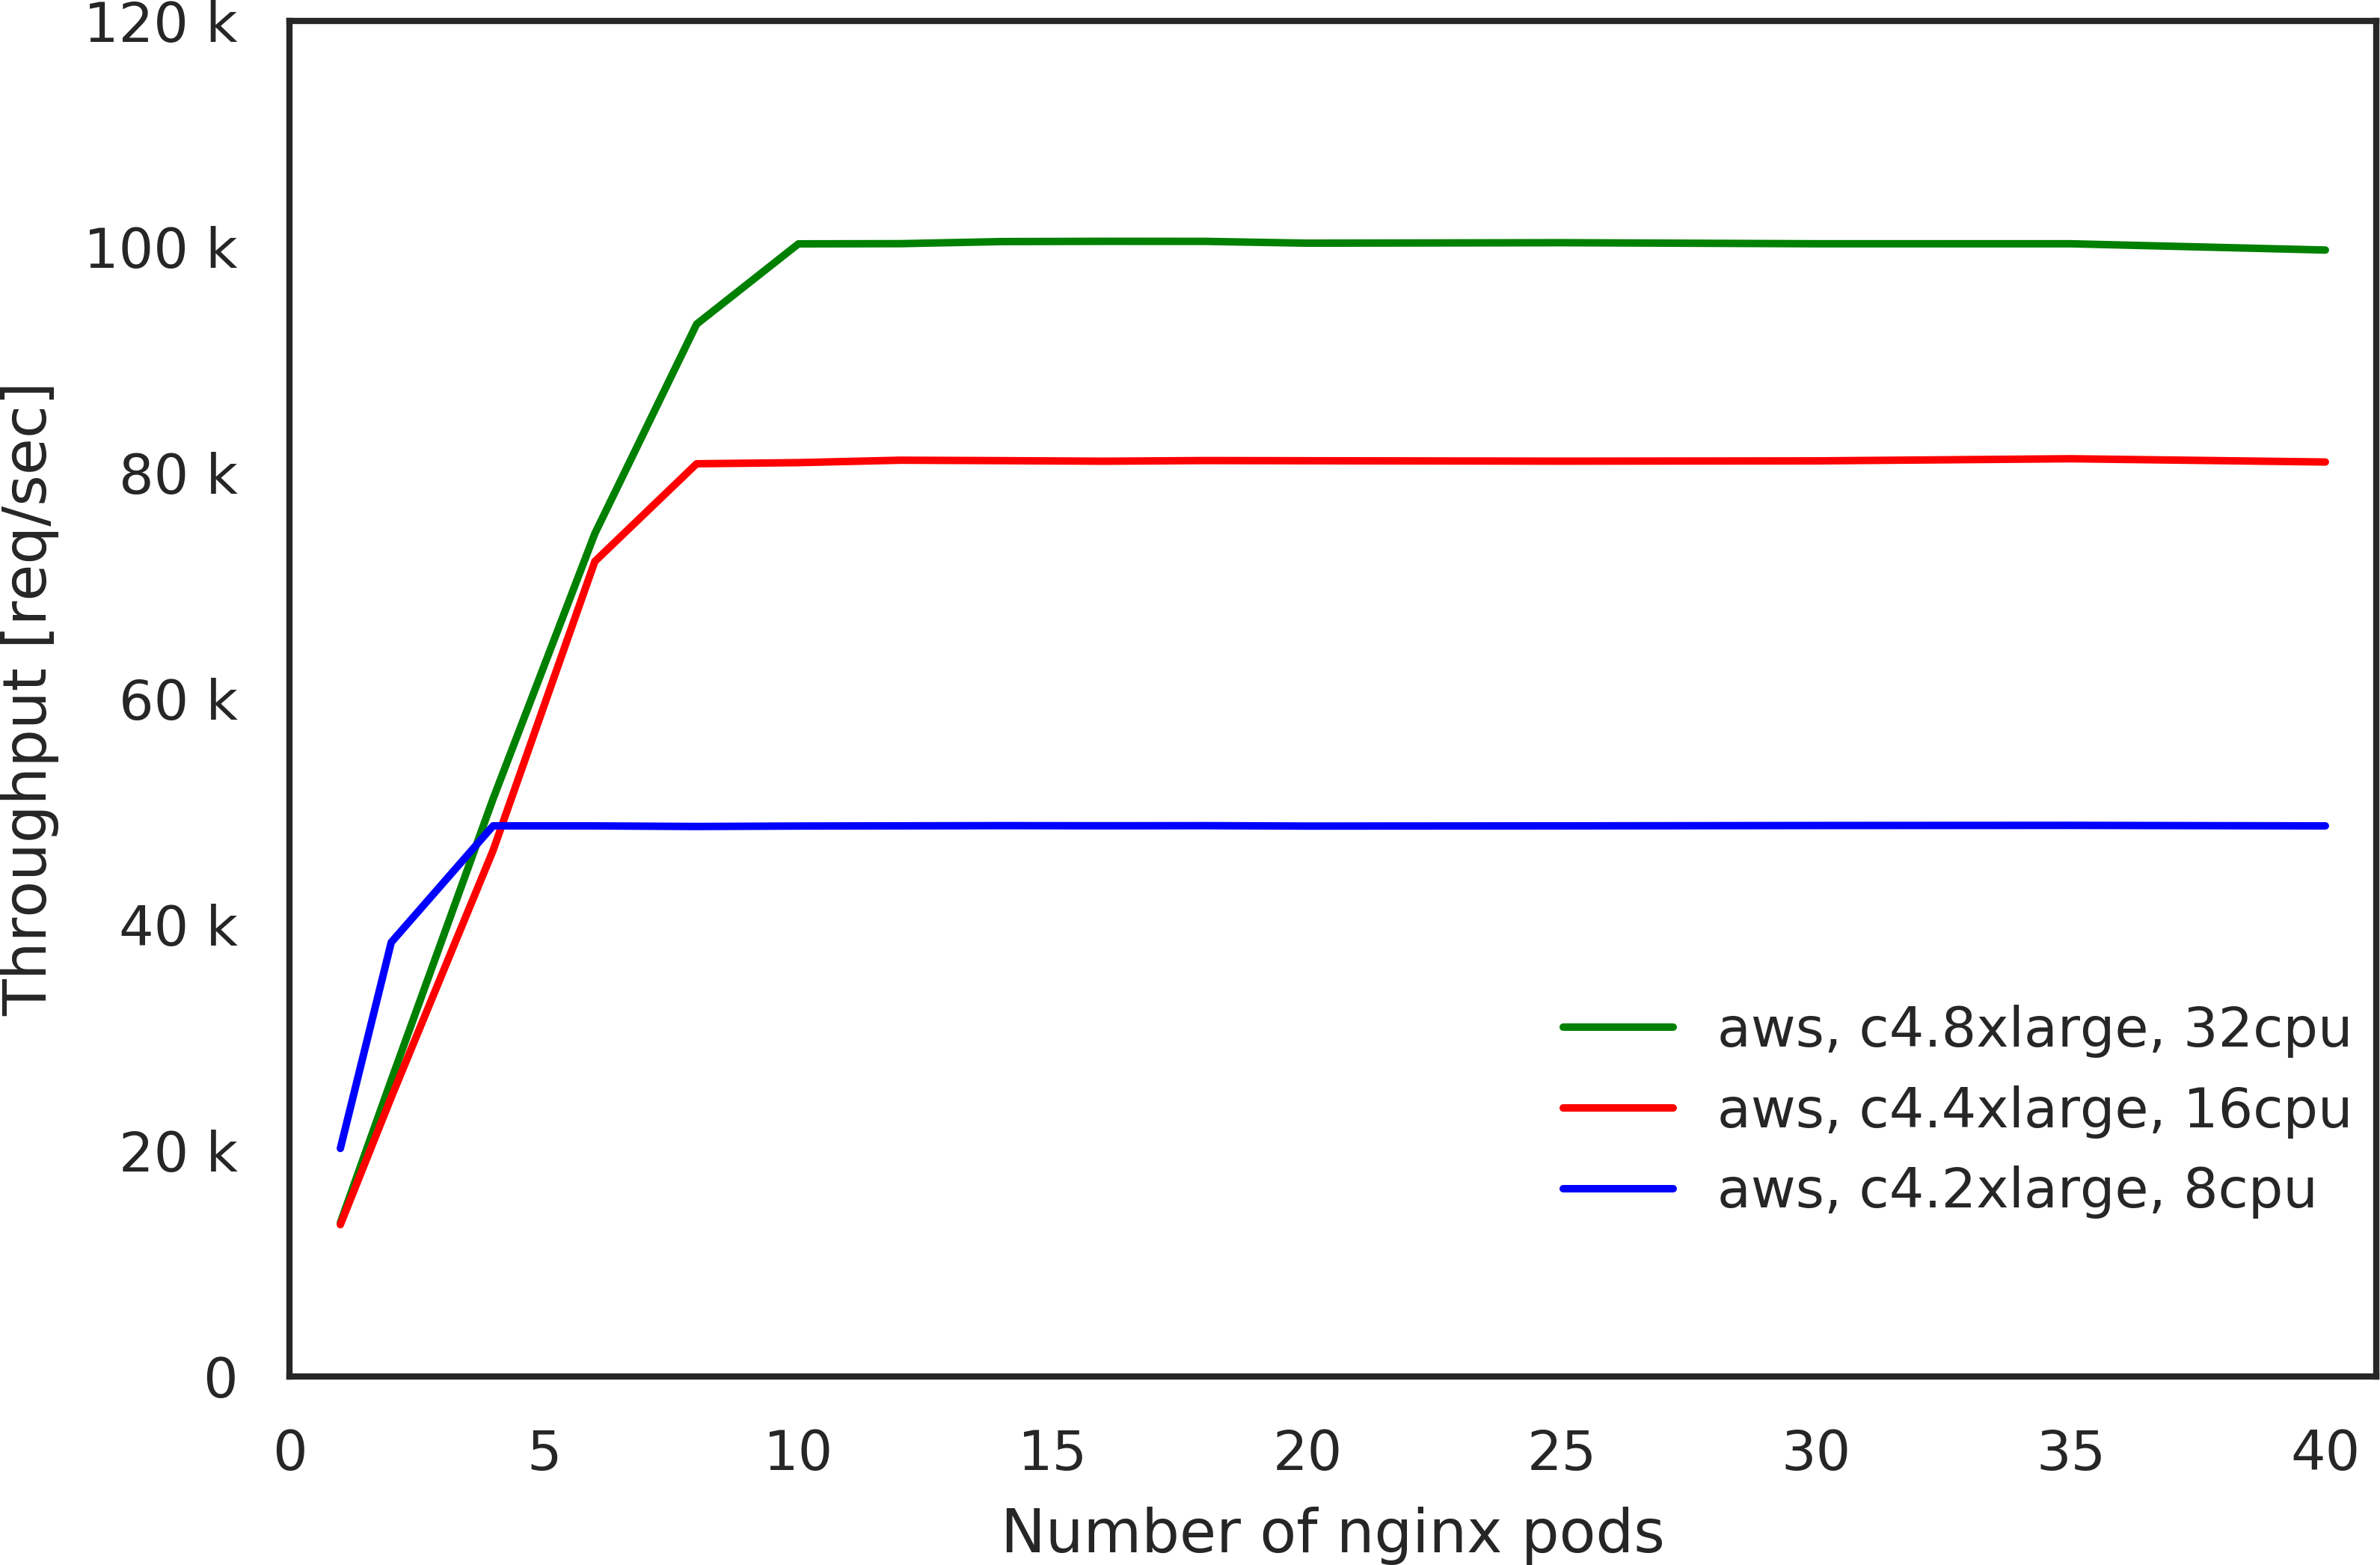
\includegraphics[width=0.75\columnwidth]{Figs/aws_c4_tp}
  \par\bigskip
  \centering
  \begin{minipage}{0.9\columnwidth}
    \caption[Throughput measurement results in AWS]{
Throughput measurement results in AWS.
The throughput increases linearly as the number of nginx {\em pod}s increases until it reaches the saturation level.
The maximum throughput is higher for instances with more virtual CPUs.
    }
    \label{fig:aws_c4_tp}
  \end{minipage}
\end{figure}

Figure~\ref{fig:gcp_all_tp} and Figure~\ref{fig:aws_c4_tp} show throughput results that are measured in GCP and AWS, respectively. 
Both results show similar characteristics as the experiment in an on-premise data center in Figure~\ref{fig:ipvs-iptables-nginx}, where throughput increased linearly to a certain saturation level that is determined by either network speed or machine specifications.
It is also seen that the performance levels are higher for load balancer nodes with more CPUs in both GCP and AWS. 
These results indicate that the proposed ipvs load balancers function properly in GCP and AWS, and hence can be run in those environments.

In general, the throughput results in the cloud environments are inferior to those in the on-premise data center, even though much more powerful CPUs are used for VMs in the cloud environment than the experiment in the on-premise data center.
For example, while the maximum throughput of the ipvs load balancer with eight physical cores was ~190K[req/sec] in the on-premise data center(Figure~\ref{fig:ipvs_mcore_proccessing}), the maximum throughput in GCP and AWS are ~160K[req/sec] and ~100K[req/sec], respectively, even with 32 and 36 virtual CPUs.
Although the author suspects that this is probably due to the inefficiency of the virtual machines as opposed to Bare Metal servers,
it is not clear what limits the maximum performance levels of cloud environments. 
The author leaves a detailed analysis for future work.

%% From the first look of the results, since changing CPU counts changed the load balancer's throughput saturation levels, we thought VM's computation power limited the performance levels.
%% However, since there are cases in the cloud environment, where changing the VM types or CPU counts also changes the network bandwidth limit, a detailed analysis is further required in the future to clarify which factor limits the throughput in the cases of these cloud environments.
%% Still, we can say that 

%\mytodo[inline]{Mention that BGP peering is unavailable in cloud , in somewhere.}

\FloatBarrier

\section{Redundancy with ECMP}

While containerizing ipvs makes it runnable in any environment, it is essential to discuss how to route the traffic to the ipvs container in a redundant and scalable manner.
The ECMP technique is expected to make the load balancers redundant and scalable since all the load balancer containers act as active.
The author examined the behavior of the ECMP routing table updates, by changing the number of the load balancers.
After that, in order to explore the scalability, the author also measured the throughput from a benchmark client with ECMP routes when multiple of the ipvs container load balancers are deployed.

\begin{figure}[h]
  \centering
  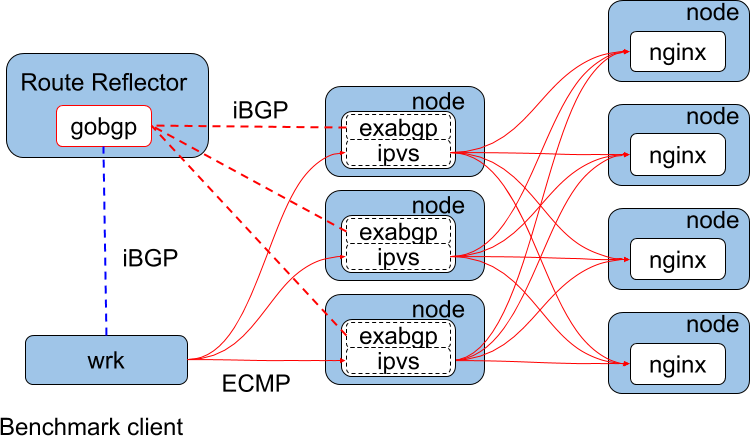
\includegraphics[width=0.9\columnwidth]{Figs/lb_ecmp_schem}

  \par\bigskip
  \centering
  \begin{minipage}{0.9\columnwidth}
    \caption[Benchmark setup for ECMP experiment]{
      Benchmark setup for ECMP experiment.
      Each load balancer pods consists of both an ipvs container and an exabgp container.
      The routing table of the benchmark client is updated by BGP protocol through a route reflector.
    }
    \label{fig:ecmp-benchmark-schem}
  \end{minipage}
\end{figure}

{
\setlength{\tabcolsep}{1em}
\renewcommand{\arraystretch}{1.2}

\begin{table}[h]
  \centering
  \begin{tabular}{ll}
    \hline 
    \multicolumn{2}{l}{[Hardware Specification]}   \\
    & CPU: Xeon E5-2450 2.10GHz x 8 (with Hyper Threading) \\
    & Memory: 32GB \\
    & NIC: Broadcom BCM5720 with 4 rx-queues, 1 Gbps \\
    & (Node x 6, Load Balancer x 4) \\
    & \\
    & CPU: Xeon E5-2450 2.10GHz x 8 (with Hyper Threading) \\
    & Memory: 32GB \\
    & NIC: Intel X550 \\
    & (Client x 1) \\
    & \\
    \multicolumn{2}{l}{[Node Software]}  \\
    & OS: Debian 9.5, linux-4.16.8 \\
    & Kubernetes v1.5.2 \\
    & flannel v0.7.0 \\
    & etcd version: 3.0.15 \\
    & \\
    \multicolumn{2}{l}{[Container Software]}   \\
    & Keepalived: v1.3.2 (12/03,2016) \\
    & nginx : 1.15.4(web server) \\
    & \\
    \multicolumn{2}{l}{[BGP Software]}   \\
    & gobgp version 1.33 (route reflector \& benchmark client) \\
    & exabgp 3.4.17 (load balancer) \\
  \hline 
  \end{tabular}
  \par\bigskip
  \centering
  \begin{minipage}{0.9\columnwidth}
    \caption[Hardware and software specifications for ECMP experiment]{
      Hardware and software specifications for ECMP experiment.
      The NIC of the benchmark client is 10 Gbps card to measure the aggregated throughput of 1Gbps load balancers.
    }
    \label{tab:ecmp-hw_sw_spec}
  \end{minipage}
\end{table}
}

Figure~\ref{fig:ecmp-benchmark-schem} shows the schematic diagram of the experimental setup. Table~\ref{tab:ecmp-hw_sw_spec} summarizes hardware and software specifications.
Notable differences from the previous throughput experiment in Figure~\ref{fig:benchmark-schem} and Table~\ref{tab:hw_machine_spec} are as follows;
1) Each load balancer pods now consists of both an ipvs container and an exabgp container.
2) The routing table of the benchmark client is updated by BGP protocol through a route reflector.
3) The NIC of the benchmark client has been changed to 10 Gbps card since now we have multiple of ipvs container load balancers that are capable of filling up 1 Gbps bandwidth.
4) Some of the software have been updated to the most recent versions at the time of the experiment.

\FloatBarrier

{
\setlength{\tabcolsep}{1em}
\renewcommand{\arraystretch}{1.2}

\begin{table}[h]

  \begin{subtable}{.9\textwidth}
    \centering
    \begin{tabular}{l}
    \hline 
    10.1.1.0/24 via 10.0.0.106 dev eth0 proto zebra metric 20 \\
    \hline
    \end{tabular}
    \caption{With single load balancer {\em pod}.}
    \label{tab:single}
  \end{subtable}

  \par\bigskip

  \begin{subtable}{.9\textwidth}
    \centering
    \begin{tabular}{ll}
      \hline
      \multicolumn{2}{l}{10.1.1.0/24 proto zebra metric 20 } \\
      \hspace{15 mm}
      & nexthop via 10.0.0.105  dev eth0 weight 1 \\
      & nexthop via 10.0.0.106  dev eth0 weight 1 \\
      & nexthop via 10.0.0.107  dev eth0 weight 1 \\
      \hline
    \end{tabular}
    \caption{With three load balancer {\em pod}s.}
    \label{tab:three}
  \end{subtable}
  
  \par\bigskip
  
  \begin{subtable}{.9\textwidth}
    \centering
    \begin{tabular}{ll}
      \hline
      \multicolumn{2}{l}{10.1.1.0/24 pro to zebra metric 20 } \\
      \hspace{15 mm}
      & nexthop via 10.0.0.107  dev eth0 weight 1 \\
      & nexthop via 10.0.0.105  dev eth0 weight 1 \\
      & nexthop via 10.0.0.106  dev eth0 weight 1 \\
      \multicolumn{2}{l}{10.1.2.0/24 proto zebra metric 20 } \\
      \hspace{15 mm}
      & nexthop via 10.0.0.107  dev eth0 weight 1 \\
      & nexthop via 10.0.0.106  dev eth0 weight 1 \\
      \hline
    \end{tabular}
    \caption{For a service with three load balancer {\em pod}s and a service with two load balancer {\em pod}s.}
    \label{tab:double_svc}
  \end{subtable}
  
  \par\bigskip
  \centering
  \begin{minipage}{0.9\columnwidth}
    \caption[ECMP routing tables]{
ECMP routing tables. All the routing rules are updated by zebra.
(a) According to this entry, packets toward 10.1.1.0/24 are forwarded to 10.0.0.106.
(b) There is a routing rule with three next hops towards 10.1.1.0/24, each of which is the node where the load balancer pods are running.
The weights of the three next-hops are all 1.
(c) There are two routing rules regarding the services with different service IPs, one with three load balancers and the other with two load balancers.
These load balancers share the same group of nodes, i.e., (10.0.0.105,10.0.0.106,10.0.0.107).
    }
    \label{tab:exabgp_routing_table}
  \end{minipage}
\end{table}
}

First, the author examined ECMP functionality by monitoring the routing table on the benchmark client.
Table~\ref{tab:exabgp_routing_table}~(\subref{tab:single}) shows the routing table entry on the router when a single load balancer pod exists.
From this entry, it is seen that packets toward 10.1.1.0/24 are forwarded to 10.0.0.106 where the load balancer pod is running.
It also shows that this routing rule is updated by zebra.
%
The routing table entry in Table~\ref{tab:exabgp_routing_table}~(\subref{tab:three}) is seen when the number of the load balancer pods is increased to three.
There are three next hops towards 10.1.1.0/24, each of which is the node where the load balancer pods are running.
The weights of the three next-hops are all 1.
The update of the routing entry was almost instant as the author increased the number of the load balancers.
%
Table~\ref{tab:exabgp_routing_table}~(\subref{tab:double_svc}) shows the case where the author additionally started new service with two load balancer pods with service addresses in 10.1.2.0/24 range.
It was possible to accommodate two services with different service IPs on the same group of nodes(10.0.0.105, 10.0.0.106, 10.0.0.107). 
The one has three load balancers and the other has two load balancers.
The update of the routing entry was almost instant as the author started the load balancers for the second service.

As far as the route withdrawal is concerned, if an exabgp is killed by SIGKILL or SIGTERM the kernel of the node close the BGP connection by sending out a packet with FIN flag to the peer gobgpd on the route reflector, and thus the route is withdrawn immediately.
The gobgp on the route reflector also periodically check the BGP connection, and if the peer exabgp container is unresponsive for more than the specified duration, “hold-time“ setting in gobgpd, it will also terminate the connection and withdraw the route.
The packets arriving within that duration will be dropped.
However, it is possible to set up the “hold-time” short enough so that the retransmitted TCP packets from the client will be forwarded correctly to functioning load balancers.

\FloatBarrier

\begin{figure}[h]
  \centering
  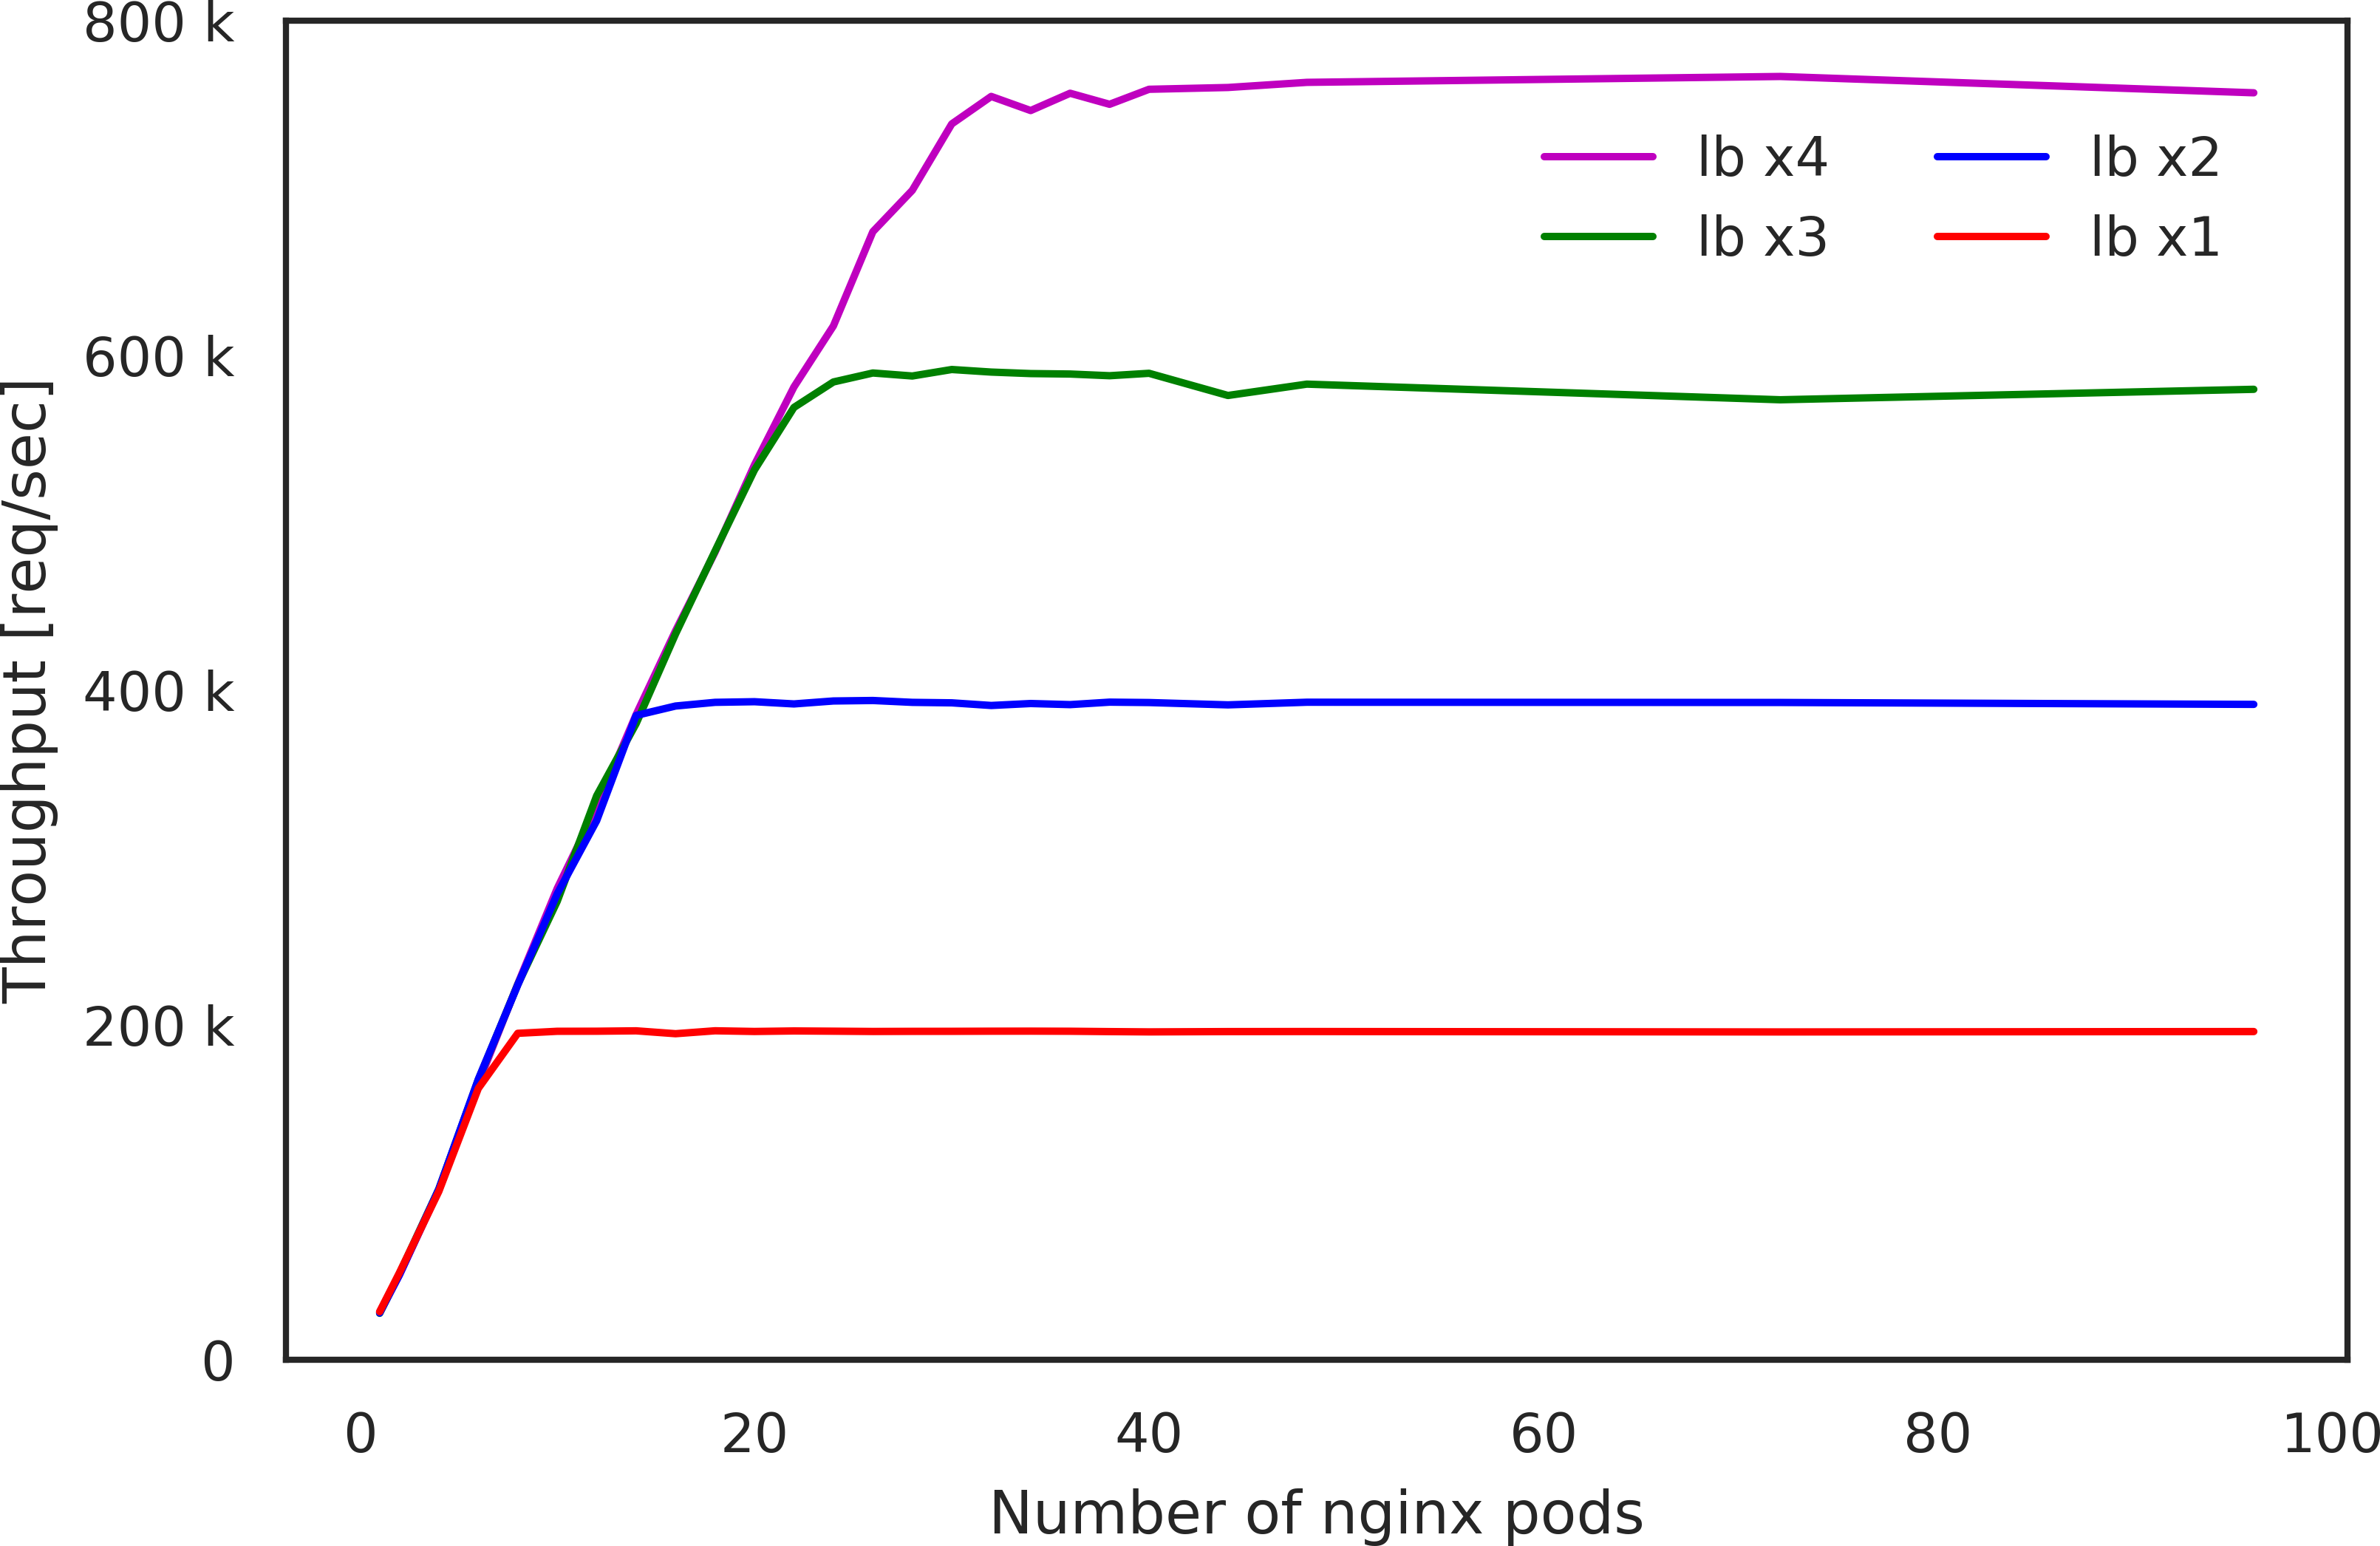
\includegraphics[width=0.9\columnwidth]{Figs/ecmp_lb_cubic}
  \par\bigskip
  \centering
  \begin{minipage}{0.9\columnwidth}
    \caption[Throughput of ECMP redundant load balancer]{
      Throughput of ECMP redundant load balancer.
      The throughputs are measured for a single load balancer(lb x1), two(lb x2), three(lb x3) and four(lb x4) load balancers.
    }
    \label{fig:ecmp_lb_cubic}
  \end{minipage}
\end{figure}

\begin{figure}[h]
  \centering
  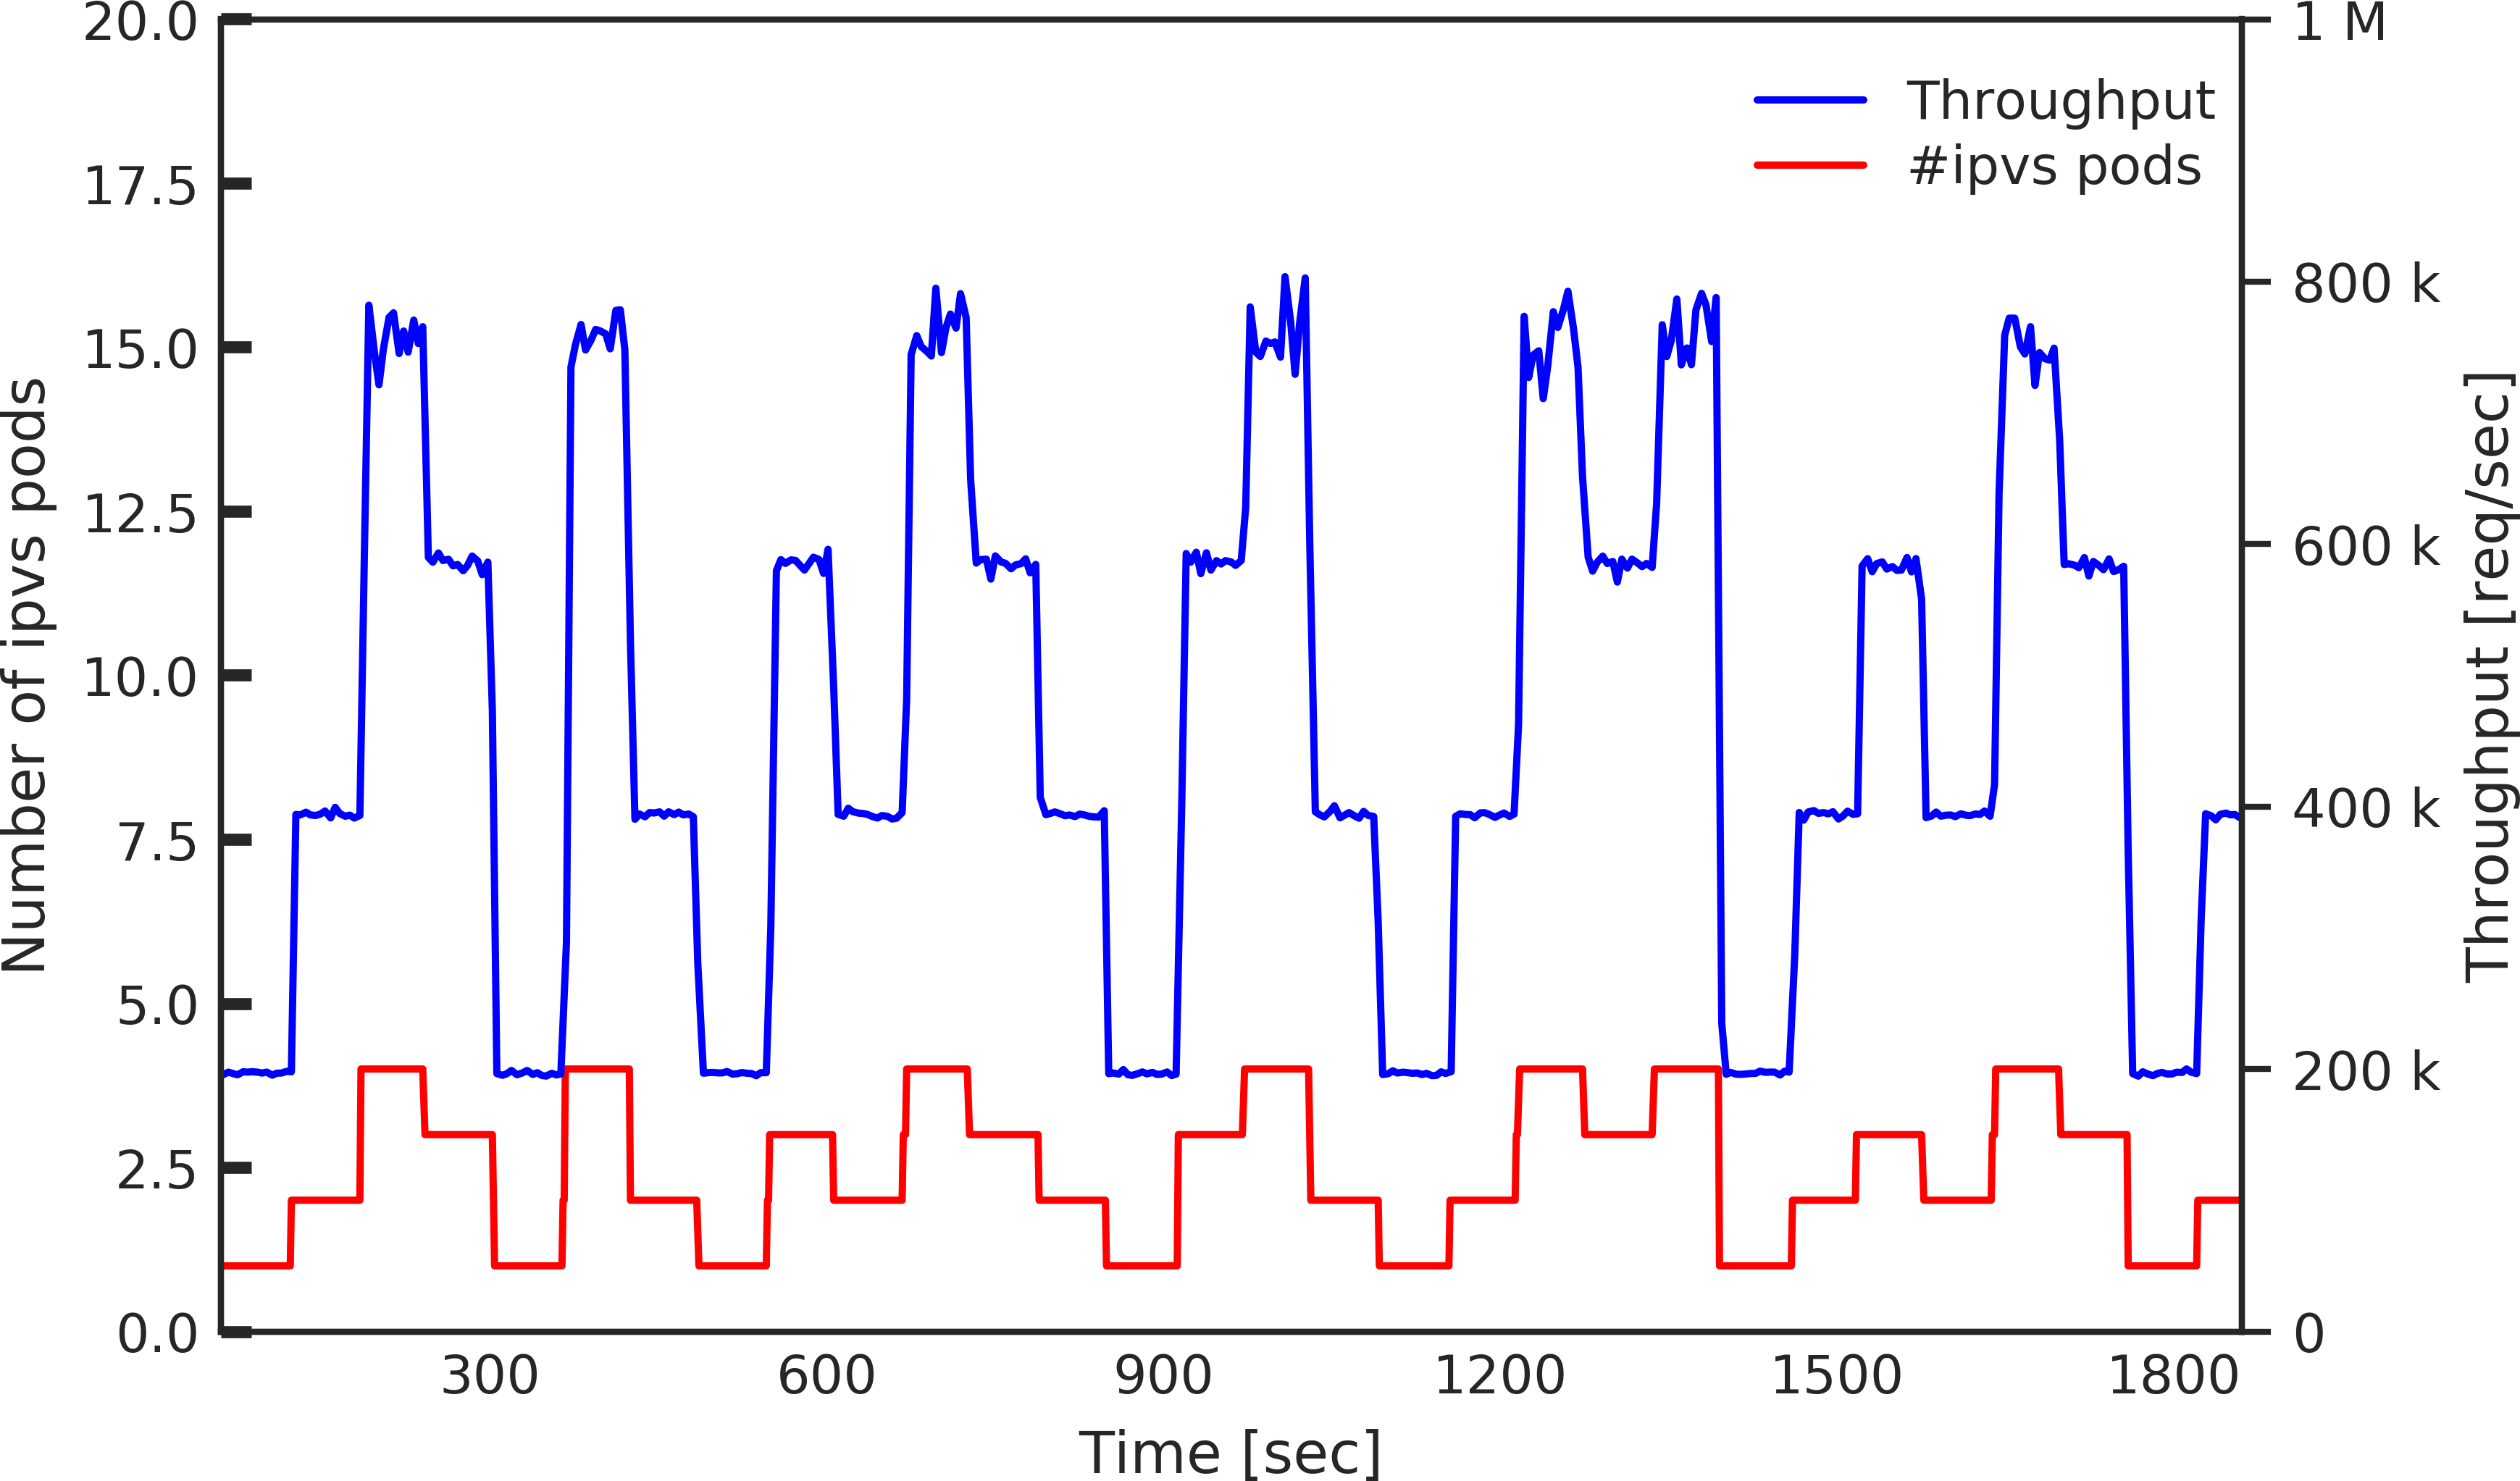
\includegraphics[width=0.9\columnwidth]{Figs/ecmp_response}
  \par\bigskip
  \centering
  \begin{minipage}{0.9\columnwidth}
    \caption[Throughput responsiveness]{
      Throughput responsiveness.
      Throughput responsiveness when the number of load balancers is changed randomly in every 60 seconds is shown.
    }
    \label{fig:ecmp_response}
  \end{minipage}
\end{figure}


\begin{figure}[h]
  \centering
  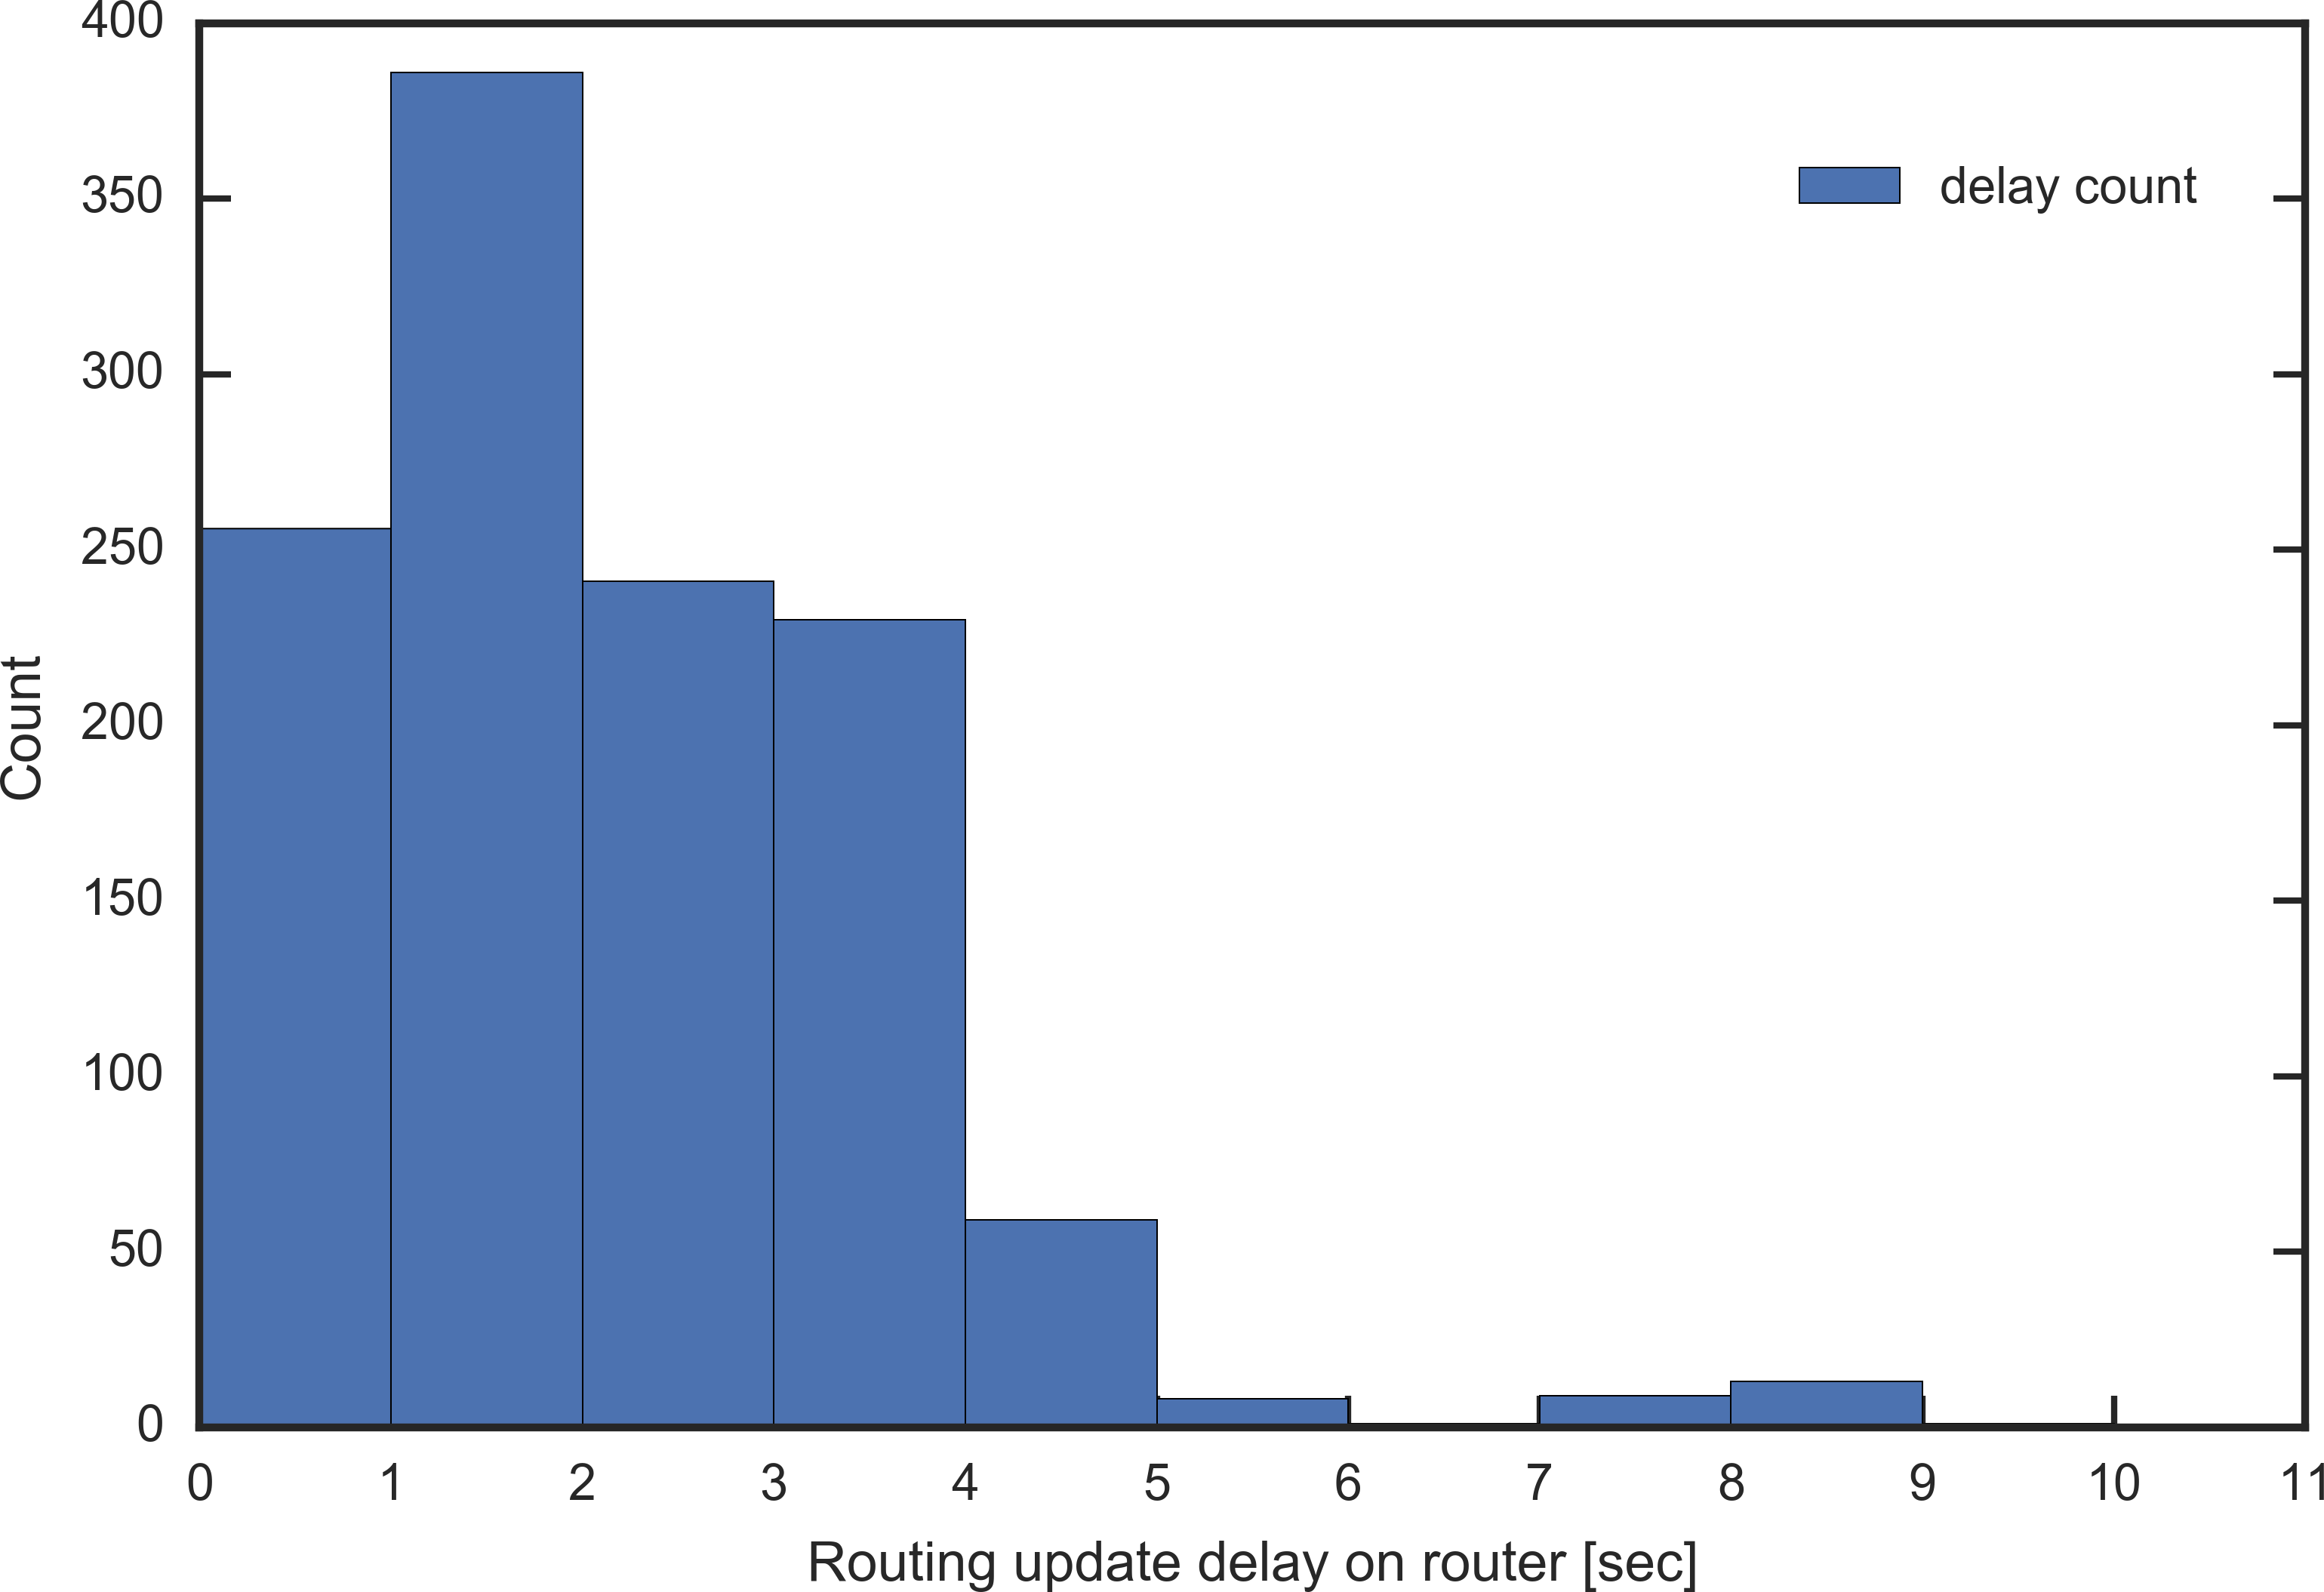
\includegraphics[width=0.9\columnwidth]{Figs/ecmp_delay_histgram}
  \par\bigskip
  \centering
  \begin{minipage}{0.9\columnwidth}
    \caption[ECMP update delay histogram]{
      ECMP update delay histogram.
      This shows the delays until the number of running ipvs pods is reflected in the routing table on the benchmark client, when the number of the ipvs pods is changed randomly every 60 seconds for 20 hours.
    }
    \label{fig:ecmp_delay_histgram}
  \end{minipage}
\end{figure}

The author also carried out throughput measurement to show that the proposed architecture increases the throughput as the number of the load balancers is increased.
Figure~\ref{fig:ecmp_lb_cubic} shows the results of the measurements.
There are four solid lines in the figure, each corresponding to the throughput result when there are one through four of the proposed load balancers.
The saturated levels, i.e. performance levels depend on the number of the ipvs load balancer pods(lb x 1 being the case with one ipvs pods, and lb x2 being two of them and as such). 
The performance level increases linearly as the number of the load balancers increases up to four of the ipvs load balancers, but does not scale further.
This is because the benchmark program uses up CPU power of the benchmark client, i.e., the CPU usage is 100\% when there are more than four load balancers.
The author expects that replacing the benchmark client with more powerful machines, or changing the experimental setup so that multiple benchmark clients can simultaneously perform the throughput measurements, will improve the performance level further.

Figure~\ref{fig:ecmp_response} shows the throughput measurement results when the author periodically changed the number of the load balancers. 
The red line in the figure shows the number of ipvs load balancer pods, which is changed randomly every 60 seconds.
The blue line corresponds to the resulting throughput.
As can be seen from the figure, the blue line nicely follows the shape of the red line.
This indicates that new load balancers are immediately utilized after they are created, and after removing some load balancers, the traffic to them is immediately directed to the existing load balancers.

Figure~\ref{fig:ecmp_delay_histgram} shows a histogram of the ECMP update delay, where the author measured the delays until the number of running ipvs pods is reflected in the routing table on the benchmark client, as the number of the ipvs pods is changed randomly every 60 seconds for 20 hours.
As can be seen from the figure, most of the delays are within 6 seconds, and the largest delay during the 20 hours experiment was 10 seconds.
The author concludes that ECMP routing update in the proposed architecture is quick enough.

\FloatBarrier

\section{Summary}\label{Conclusions}

In this chapter, the performance levels of the proposed load balancer have been evaluated. 
The author carried out throughput measurement to verify the feasibility of the load balancer and verified the followings;
(1) The throughput of the proposed load balancer linearly increases as the number of nginx {\em pod}s increases, and then it eventually saturates, indicating the load balancer functions properly.
(2) The throughput maximum depends on the multicore packet processing settings and overlay network settings.
%
(3) The throughput of the ipvs in a container is equivalent to that of the iptables DNAT as a load balancer, in 1Gbps network environment.
(4) The throughput of the ipvs container can be further improved up to 1.5 times by utilizing ipvs-tun mode, i.e., L3DSR settings.
(5) The ipvs container is able to run and function properly, both in GCP and AWS.
(6) The ECMP routing update in the proposed architecture is properly functioning and quick enough.
(7) The linear scalability of the ECMP throughput has been confirmed up to 4x of single load balancer throughput.
From these results, the author concludes that the proposed load balancer is portable, redundant and scalable while providing 1.5 times better throughput than iptables DNAT in 1Gbps network environment.


%\chapter{Further Improvement}\label{chapter:Further Improvement}
\chapter{Validity in faster network}\label{chapter:Further Improvement}

It the previous chapter the proposed load balancer is verified to be portable, redundant and scalable in 1Gbps network.
It is also important to investigate its validitys in 10Gbps network.
In this chapter the performance level of the proposed load balancer is evaluated.
The author carries out throughput measurements of ipvs, ipvs-tun, and iptables DNAT in 10Gbps environment.
The author clarifies the reasons for performance limitations and discusses improvement.
The author also proposes a novel software load balancer using eXpress Data Plane(XDP) technology and presents preliminary experimental results.

\section{Throughput measurement in 10G network}

In order to evaluate the performance levels of the proposed load balancer in a 10Gbps network environment, the author carried out throughput measurements.
Table~\ref{tab:hw_sw_spec_10g} summarizes the hardware and software specification used in the experiment.
Bare metal servers with Intel X550 network card was used.
The X550 NIC has a maximum of 64 rx-queues, and 16 of them are activated by the driver at the boot time since there are 16 logical CPUs.
The setting \enquote{(RSS, RPS)=(on, off)} is used because interrupts from each of 16 rx-queues can be assigned to separate logical cores.
And hence, packet processing is distributed to all of the 16 logical cores, which results in the best performance in most of the cases.
The host-gw mode is used as the backend mode of the flannel overlay network.

{
\setlength{\tabcolsep}{1em}
\renewcommand{\arraystretch}{1.2}

\begin{table}[h]
  \centering
  \begin{tabular}{ll}
    \hline 
    \multicolumn{2}{l}{[Hardware Specification]}   \\
    & CPU: Xeon E5-2450 2.10GHz x 8 (with Hyper Threading) \\
    & Memory: 32GB \\
    & NIC: Intel X550 with 64 rx-queues (16 activated), 10 Gbps \\
    & (Node x 6, Load Balancer x 1, Client x 1)) \\
    & \\
    \multicolumn{2}{l}{[Node Software]}  \\
    & OS: Debian 9.5, linux-4.16.8 \\
    & Kubernetes v1.5.2 \\
    & flannel v0.7.0 \\
    & etcd version: 3.0.15 \\
    & \\
    \multicolumn{2}{l}{[Container Software]}   \\
    & Keepalived: v1.3.2 (12/03,2016) \\
    & nginx : 1.15.4(web server) \\
  \hline 
  \end{tabular}
  \par\bigskip
  \centering
  \begin{minipage}{0.9\columnwidth}
    \caption[Hardware and software specifications for 10Gbps experiment]{
      Hardware and software specifications for 10Gbps experiment.
      There are 16 rx-queues activated for the NIC, to match the number of logical CPUs.
    }
    \label{tab:hw_sw_spec_10g}
  \end{minipage}
\end{table}
}

\begin{figure}[h]
  \begin{subfigure}[t]{\columnwidth}
    \centering
    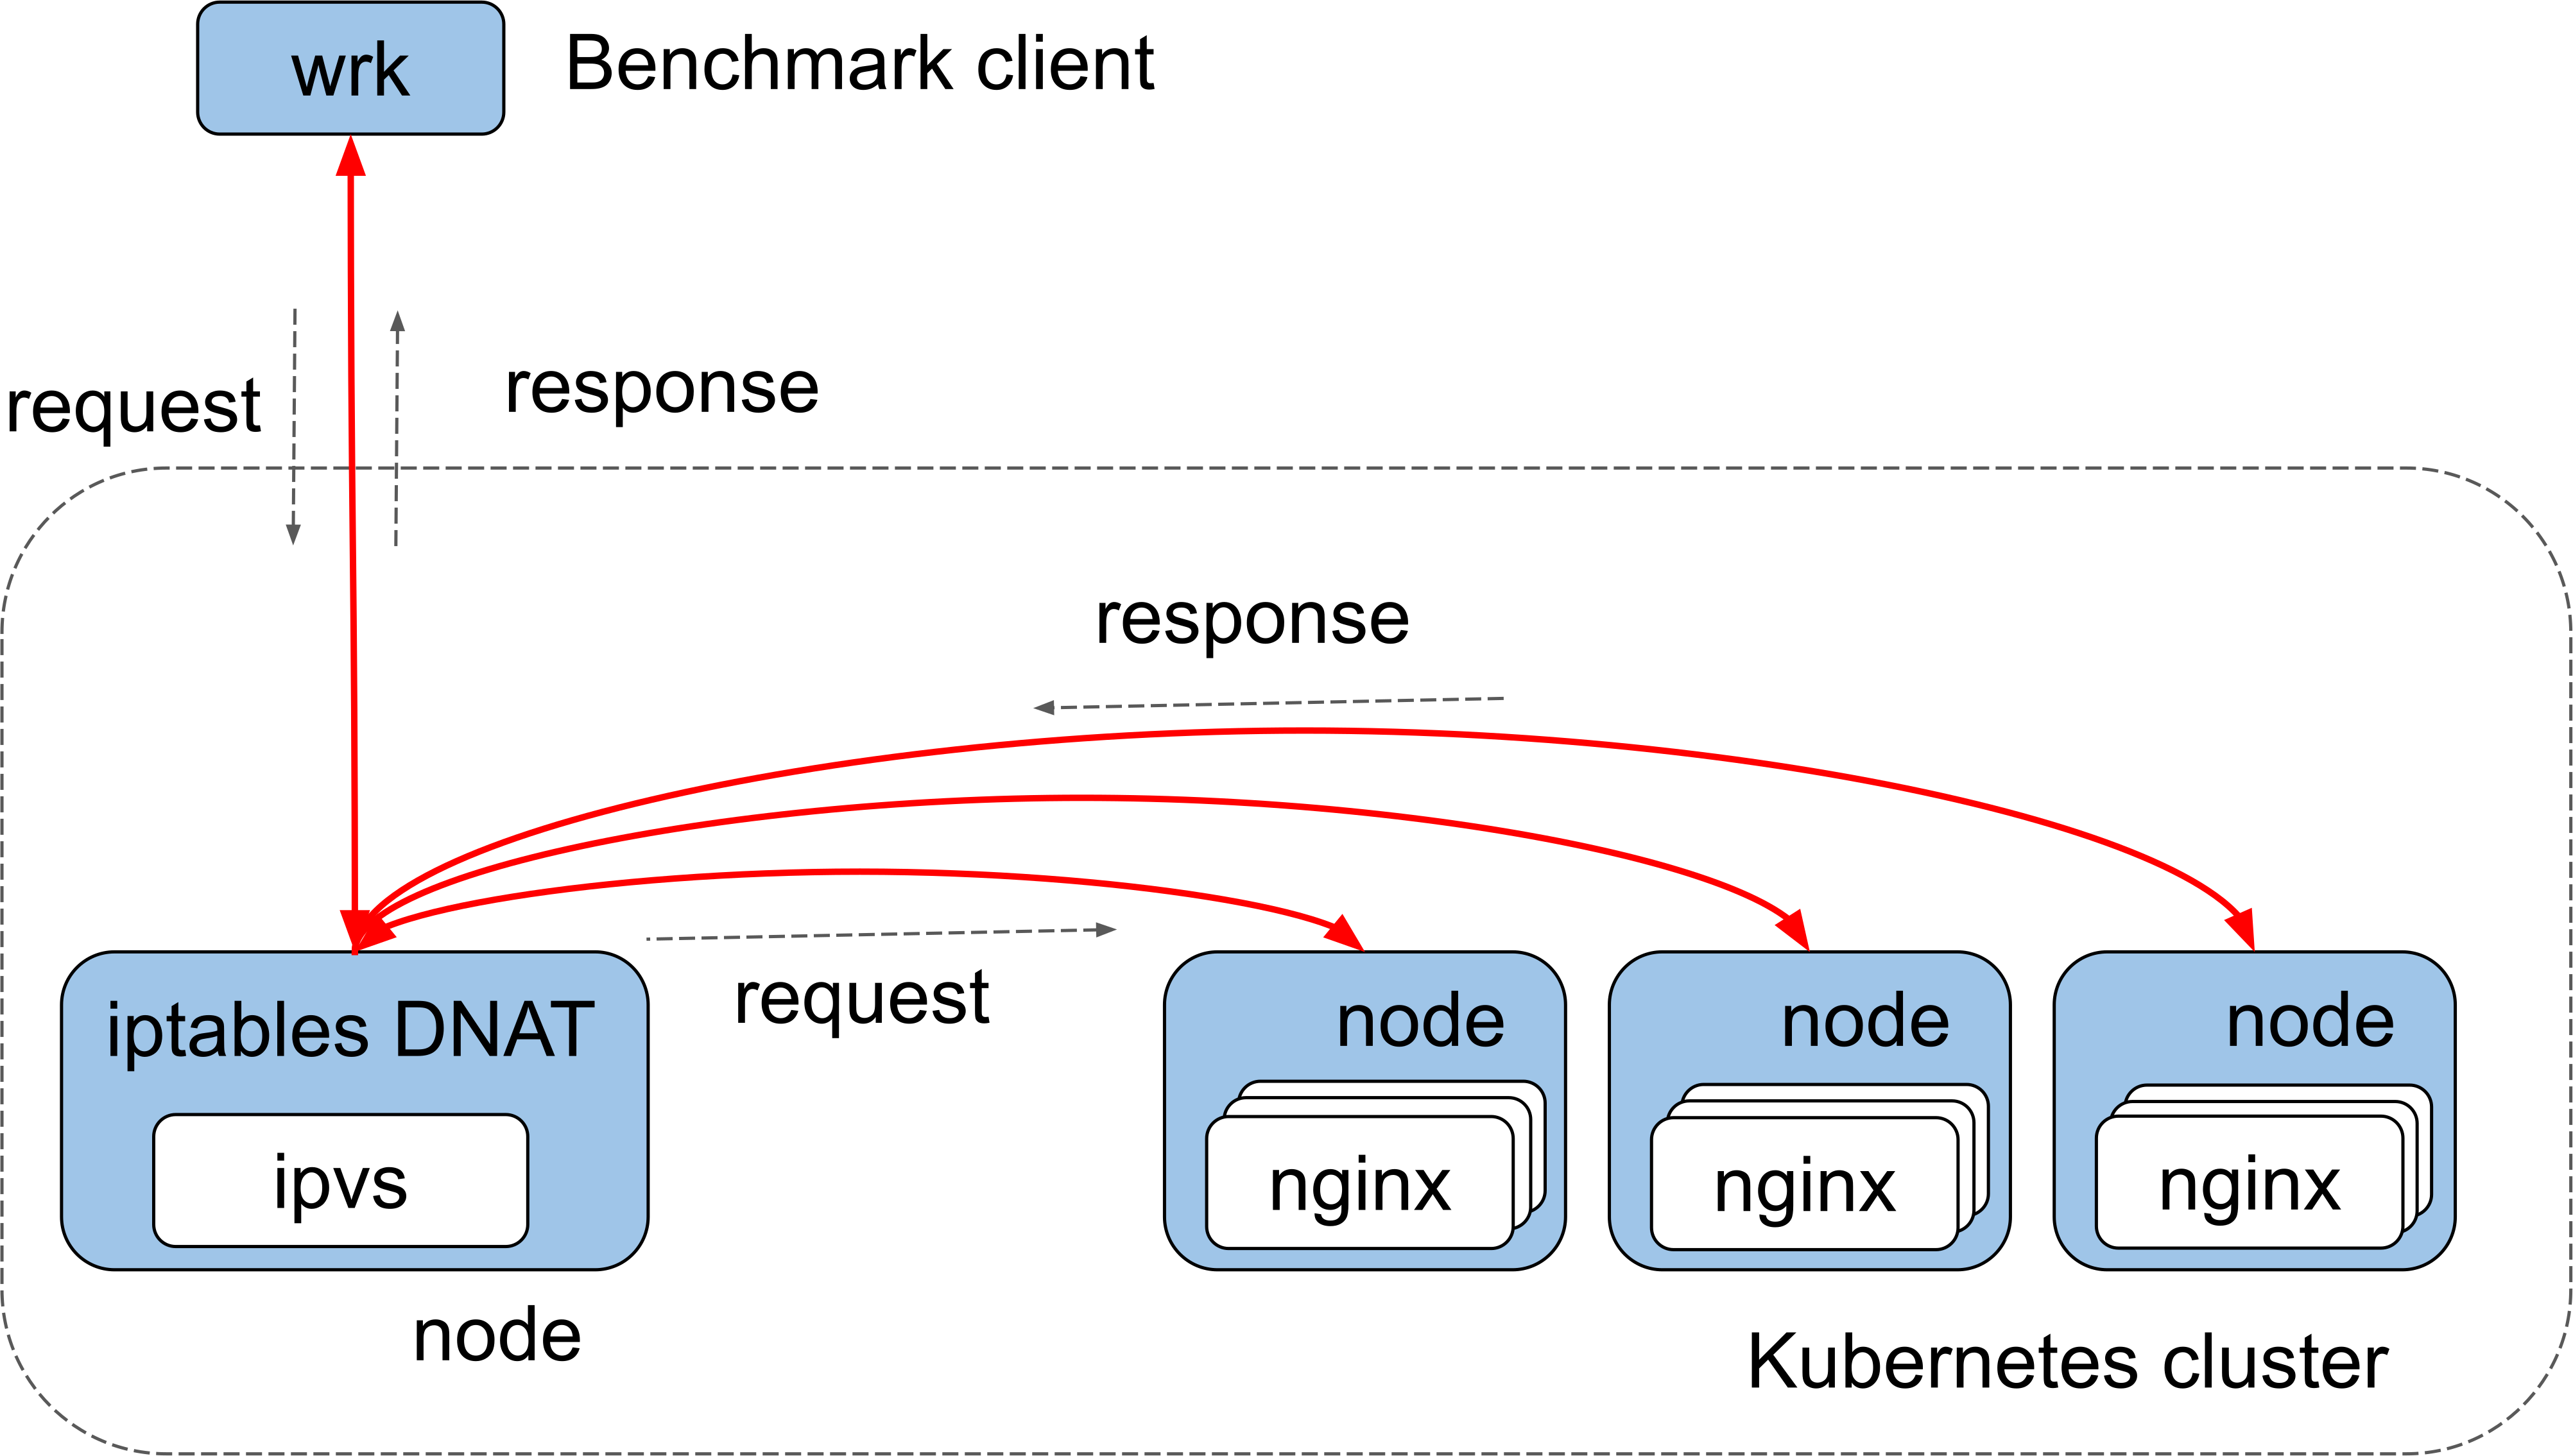
\includegraphics[width=0.8\columnwidth]{Figs/benchmark-schem-10g-nat}
    \par\bigskip
    \centering
    \begin{minipage}{0.9\columnwidth}
      \caption{}
      \label{fig:benchmark-schem-10g-nat}
    \end{minipage}
  \end{subfigure}

  \begin{subfigure}[t]{\columnwidth}
    \centering
    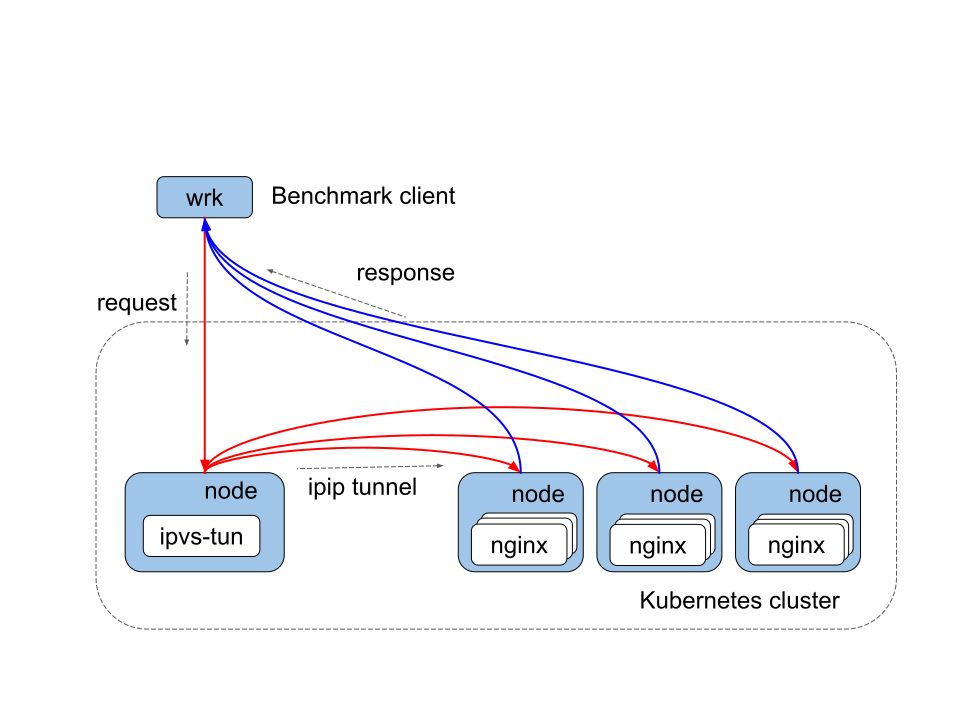
\includegraphics[width=0.8\columnwidth]{Figs/benchmark-schem-10g-dsr}
    \par\bigskip
    \centering
    \begin{minipage}{0.9\columnwidth}
      \caption{}
      \label{fig:benchmark-schem-10g-dsr}
    \end{minipage}
  \end{subfigure}

  \par\bigskip
  \centering
  \begin{minipage}{0.9\columnwidth}
    \caption[Benchmark setups in 10 Gbps experiment]{
      Benchmark setups in 10 Gbps experiment.
      (a) The setup used in throughput measurements of ipvs and iptables DNAT.
      The request and response packets both go through the load balancer node.
%      There is a bottleneck at the NIC of the load balancer node.
      (b) The setup used in throughput measurements of ipvs-tun.
      The response packets for ipvs-tun, return directly to the benchmark client.
%      The bottleneck is at the NIC of the benchmark client.
    }
    \label{fig:benchmark-schem-10g}
  \end{minipage}
\end{figure}

Figure~\ref{fig:benchmark-schem-10g} show experimental setups for the throughput measurements.
Multiple nginx {\em pods} are deployed on multiple nodes as web servers in the Kubernetes cluster.
In each nginx {\em pod}, single nginx web server program that returns the IP address of the {\em pod} itself is running.
The author then launched ipvs and ipvs-tun pod as load balancers on one of the nodes, after that, the author performed the throughput measurement changing the number of the nginx web server pods.
On every Kubernetes node, there are iptables DNAT rules that function as an internal load balancer.
The author also measured throughput of the iptables DNAT as a load balancer.
The throughput is measured by sending out HTTP requests from the wrk towards a load balancer and by counting the number of responses the benchmark client received.
In the case of the ipvs-tun, i.e., the tunneling mode of ipvs, the response packets follow the different route than the case of conventional ipvs and iptables DNAT.
As a result, the better performance level is expected for ipvs-tun since the load balancer node only has to deal with request packets of the traffic.

\FloatBarrier

Figure~\ref{fig:ipvs_l3dsr_10g} shows the throughput results of ipvs, ipvs-tun and iptables DNAT in 10Gbps environment.
The general characteristics of a load balancer, where the throughput increases linearly to a saturation level as the number of nginx container increases, can be seen.
The maximum throughput of each load balancer is limited by either packet forwarding efficiency of the software load balancer itself or the bandwidth of the network.
The maximum throughput level of the iptables DNAT is close to 780k [req/sec], where the CPU usage of the benchmark client was 100\%.
The maximum throughput levels of ipvs and ipvs-tun are less than that of iptables DNAT. 

\begin{figure}[h]
  \centering
  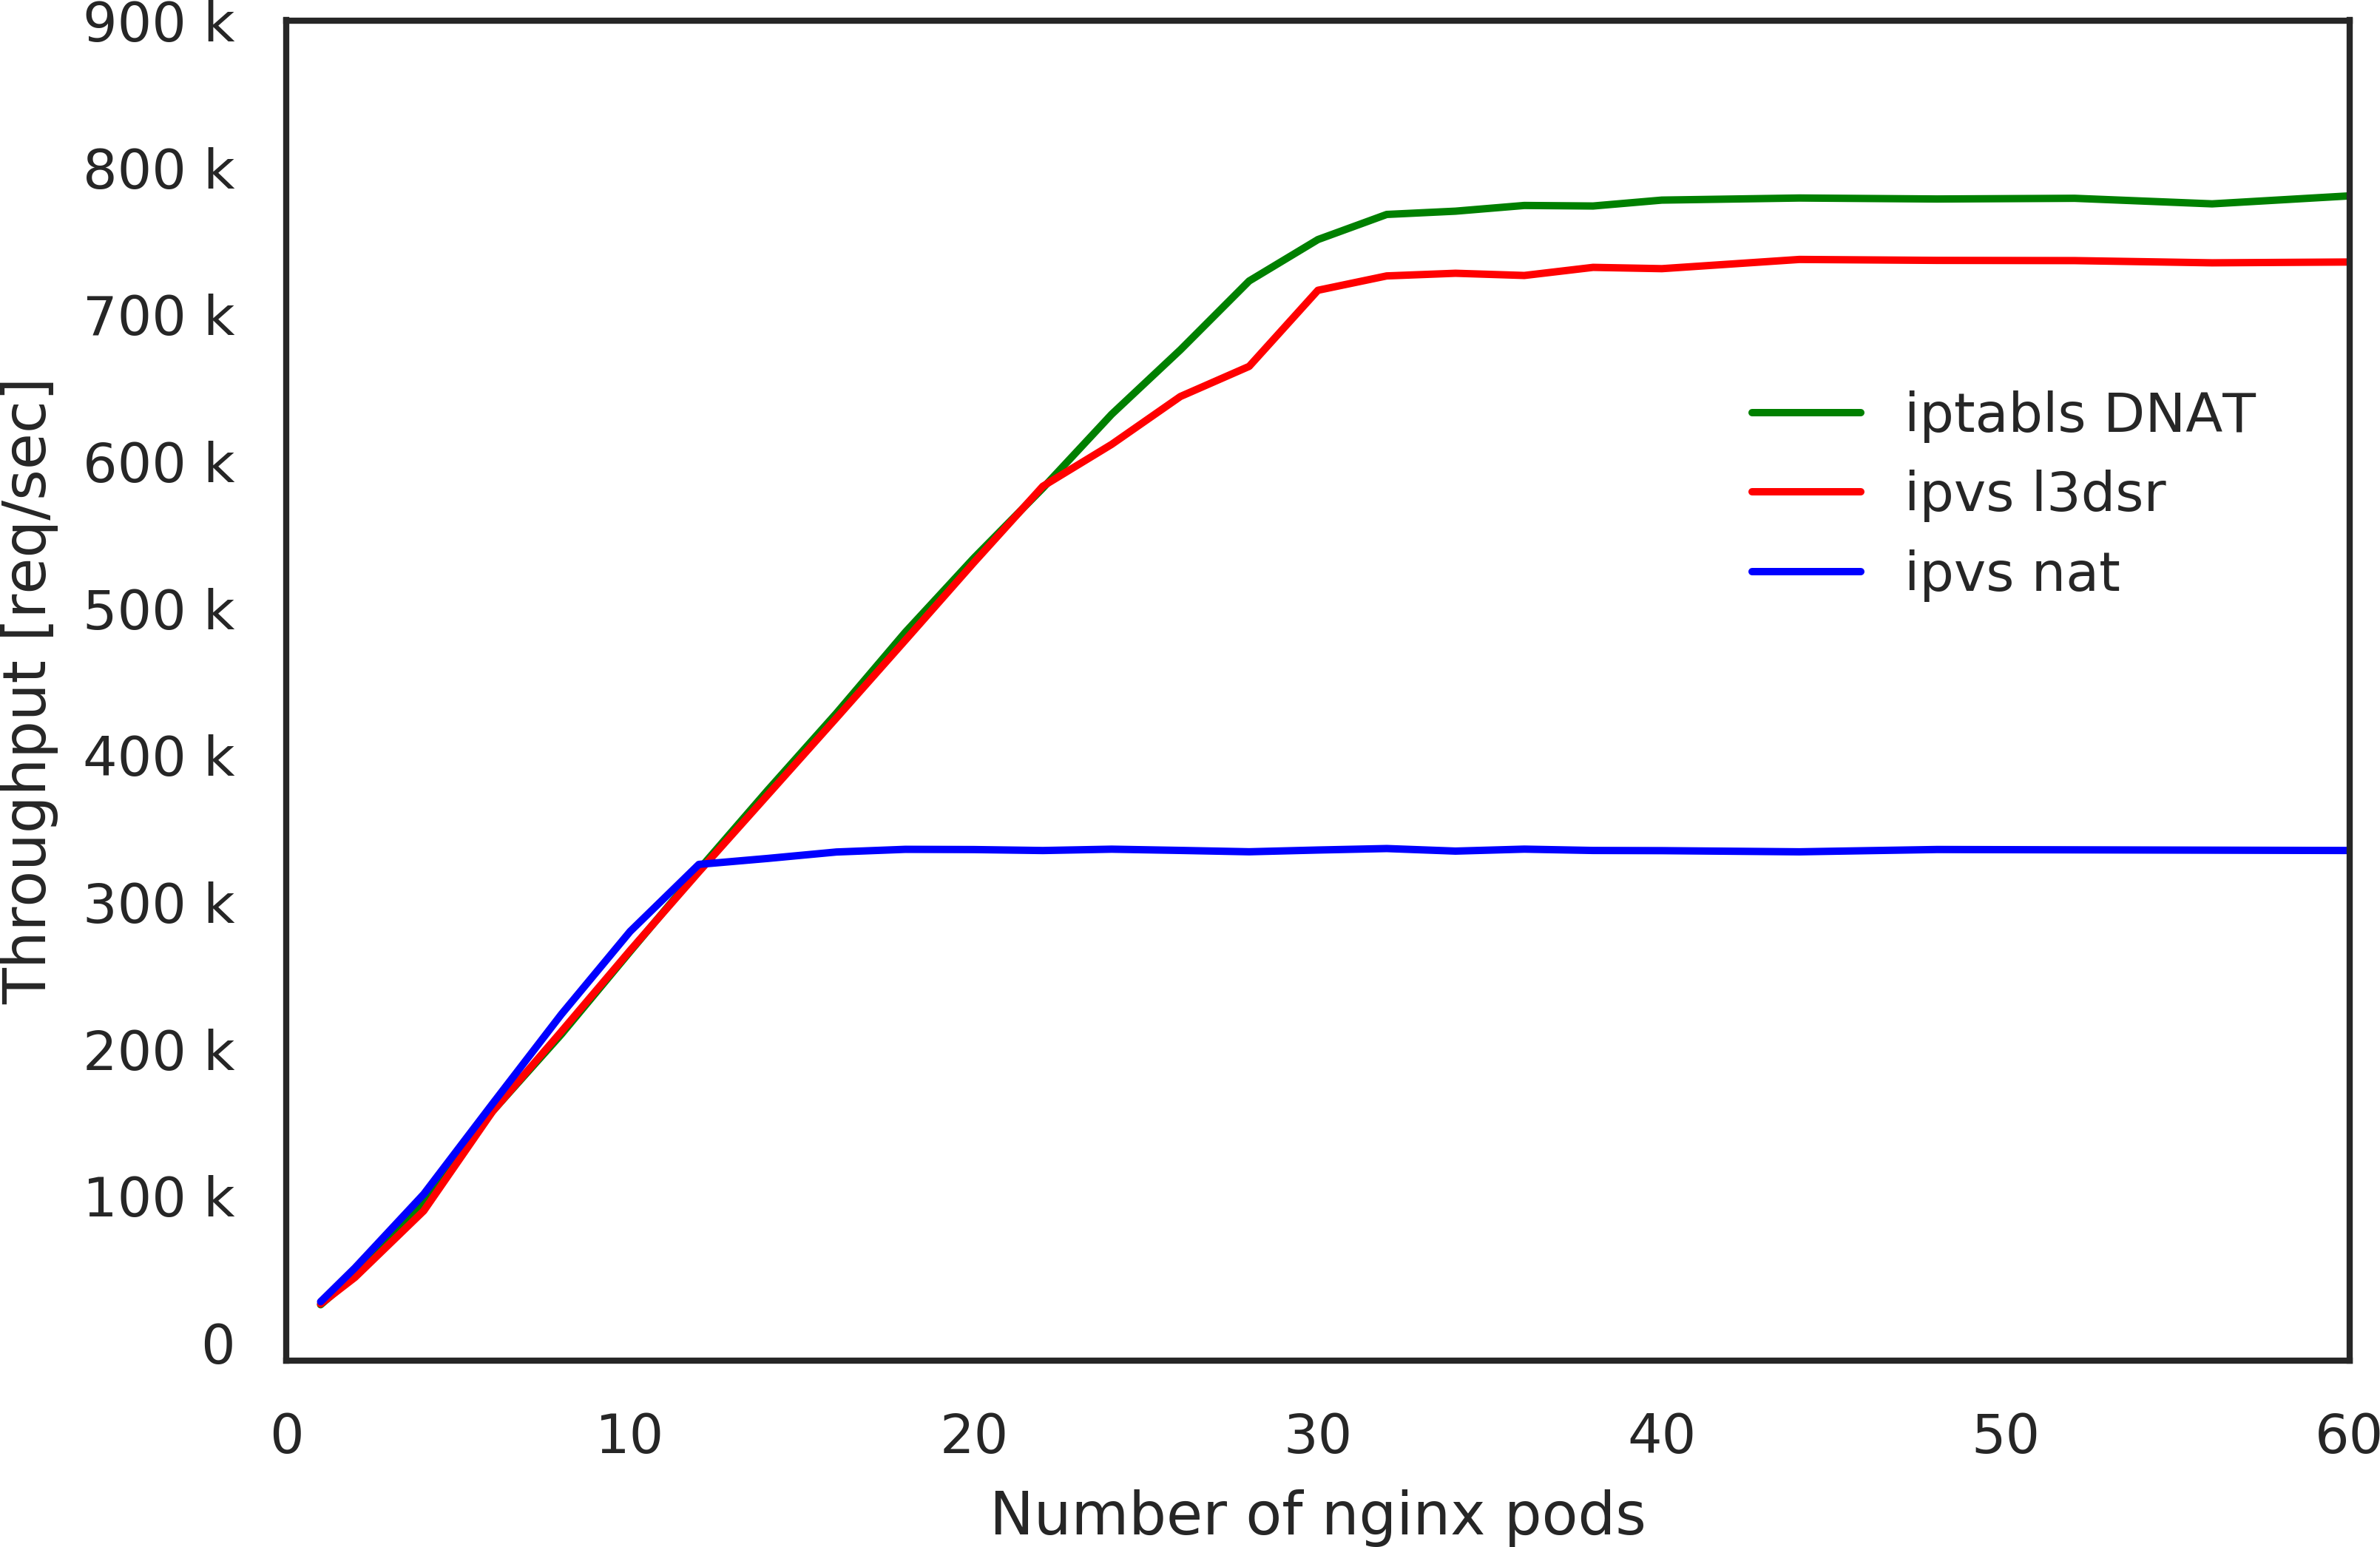
\includegraphics[width=0.8\columnwidth]{Figs/ipvs_l3dsr_10g}
  \par\bigskip
  \centering
  \begin{minipage}{0.9\columnwidth}
    \caption[Throughput of load balancers in 10 Gbps]{
      Throughput of load balancers in 10 Gbps.
      The iptables DNAT rules exist in the node net namespace.
      The ipvs and ipvs-tun are in containers.
      The throughput of the iptables DNAT is the highest.
    }
    \label{fig:ipvs_l3dsr_10g}
  \end{minipage}
\end{figure}

Figure~\ref{fig:ipvs_l3dsr_10g} shows comparison of CPU usage between load balancers.
CPU usages are sampled on the load balancer nodes at the time of the throughput measurement using a program called dstat\cite{wieers2019dstat}.
It is seen that ipvs-tun uses less CPU resource than ipvs because the load balancer node does not have to deal with the response packets.
The iptables DNAT uses even less CPU resource than ipvs and ipvs-tun.
Possible reasons for the lesser performance levels for ipvs are as follows;
(1) It is possible that the ipvs and ipvs-tun program themselves are less efficient than iptables DNAT.
(2) The network setup for the container, i.e., bridge+veth may be causing the overhead.
While iptables DNAT rules exist in node net namespace, proposed ipvs and ipvs-tun exist in container net namespace.
In order to clarify which of these is the true reason for the performance difference, the author carried out throughput measurement for ipvs and ipvs-tun without using the container network, i.e., in node net namespaces.

\begin{figure}[h]
  \centering
  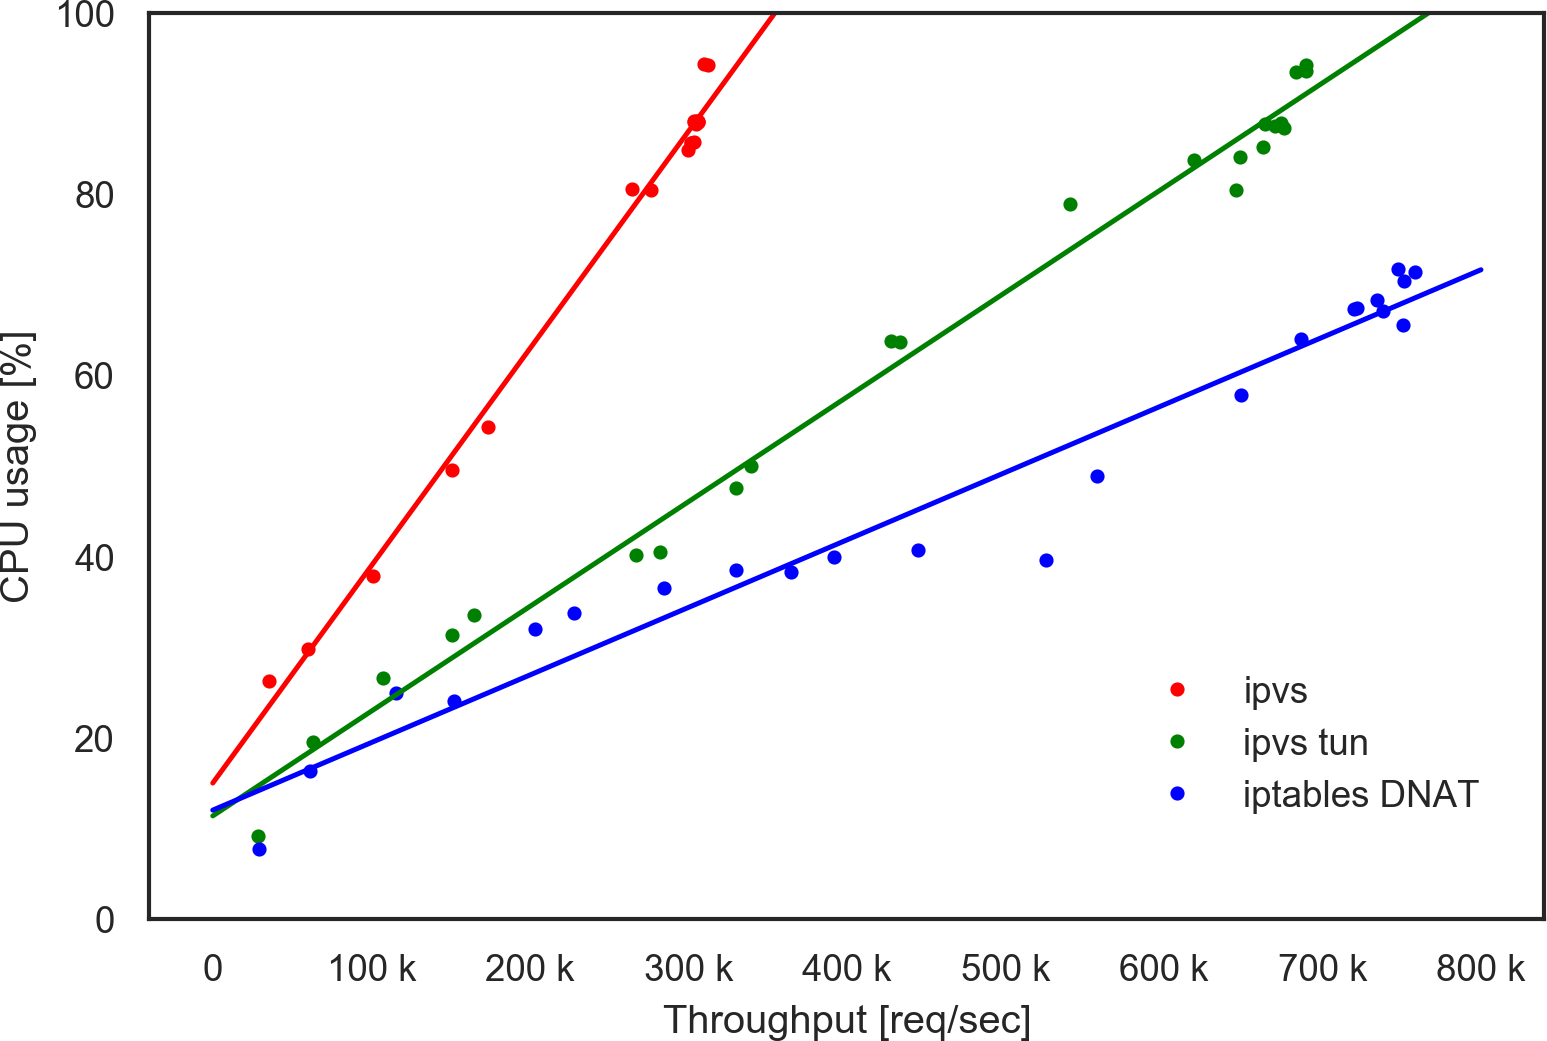
\includegraphics[width=0.8\columnwidth]{Figs/cpu_usage_10g}
  \par\bigskip
  \centering
  \begin{minipage}{0.9\columnwidth}
    \caption[CPU usage of load balancers in containers]{
      CPU usage of load balancers in containers.
      The iptables DNAT rules exist in the node net namespace.
      The ipvs and ipvs-tun are in containers.
      The iptables DNAT consumes the smallest amount of the CPU resource.
    }
    \label{fig:cpu_usage_10g}
  \end{minipage}
\end{figure}

\FloatBarrier

\subsubsection{Performance comparison in node net namespace}

The ipvs and ipvs-tun load balancers were setup on one of the nodes. 
The load balancing rules were created in the node namespaces, and then throughput measurement were carried out.

Figure~\ref{fig:ipvs_l3dsr_10g_node_ns} shows the throughput of ipvs and ipvs-tun in the node net namespace together with the throughput of the iptables DNAT.
The throughputs of the ipvs and ipvs-tun are improved from the previous results.
The throughput of the ipvs-tun is almost identical to that of iptables DNAT.
Since the CPU usages of the benchmark client were almost 100\% at the saturated throughput for ipvs and iptables DNAT, the actual maximum throughputs of these can be higher than this level.
On the other hand, the throughput of ipvs is still less than those of ipvs-tun and iptables DNAT.

\begin{figure}[h]
  \centering
  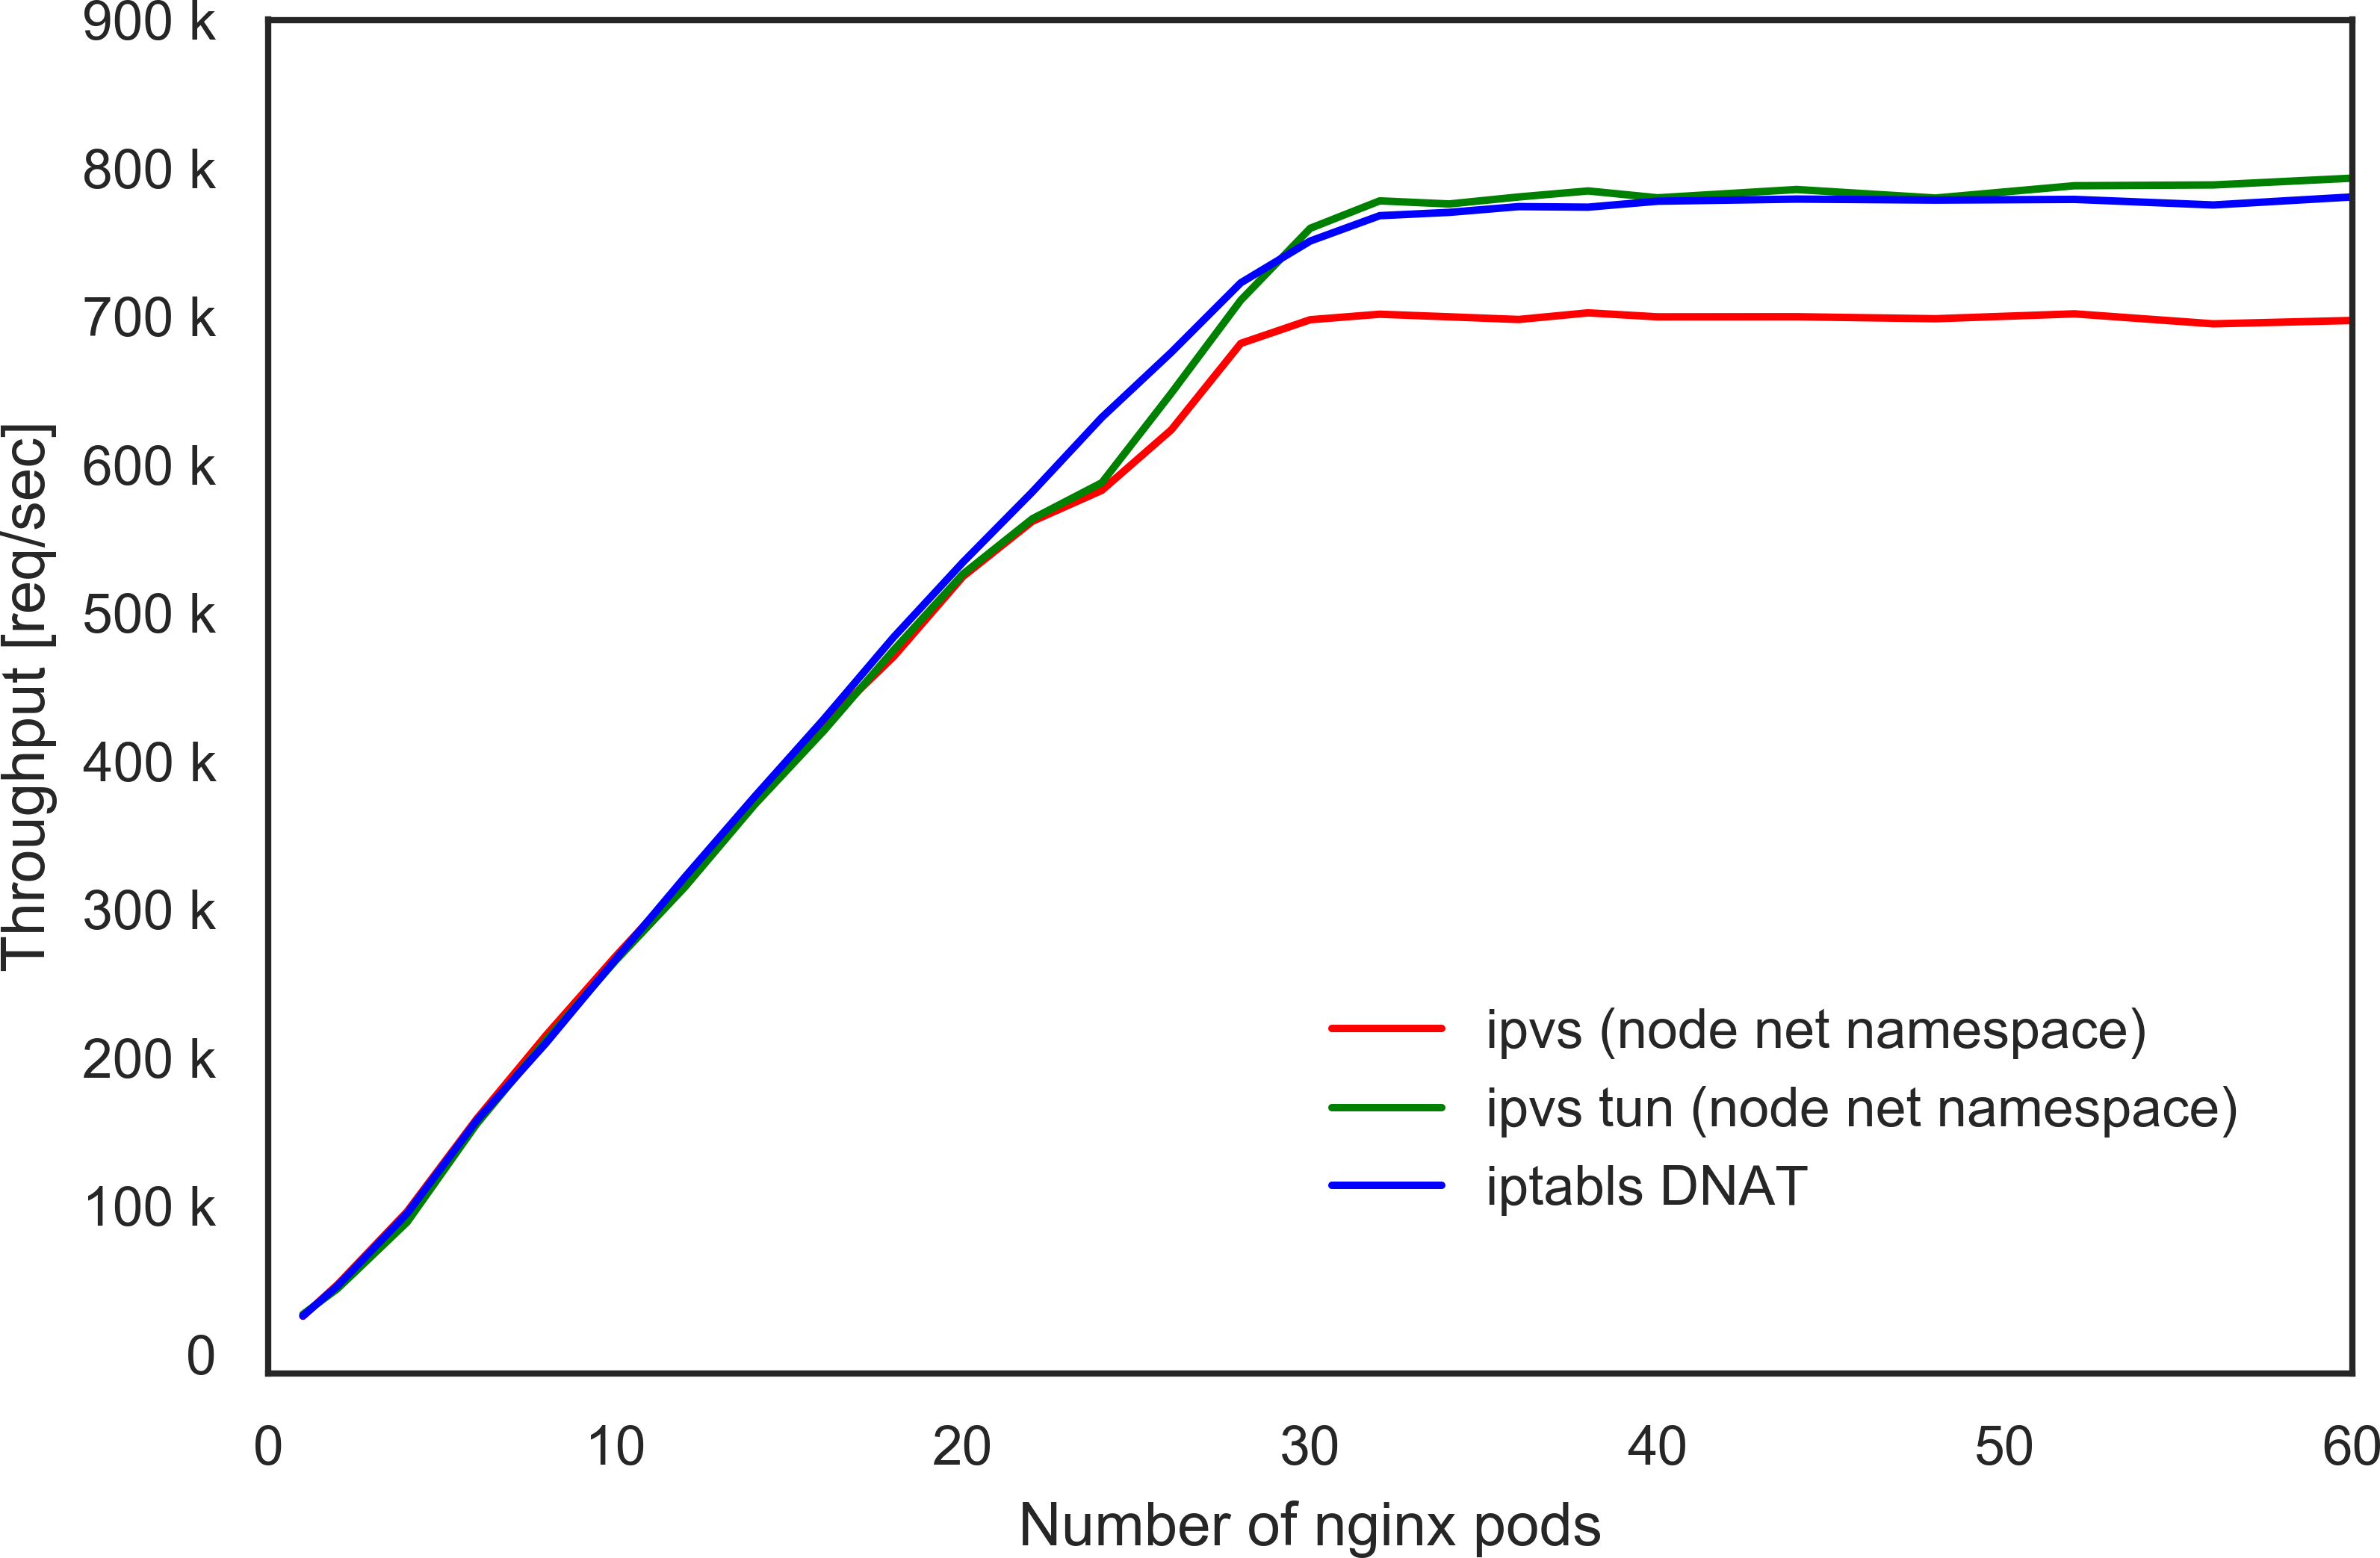
\includegraphics[width=0.8\columnwidth]{Figs/ipvs_l3dsr_10g_node_ns}
  \par\bigskip
  \centering
  \begin{minipage}{0.9\columnwidth}
    \caption[Throughput of load balancers in node namespace]{
      Throughput of load balancers in node namespace.
      The performance levels of the ipvs and ipvs-tun are greatly improved from those in Figure~\ref{fig:ipvs_l3dsr_10g} by placing them in node net namespace.
    }
    \label{fig:ipvs_l3dsr_10g_node_ns}
  \end{minipage}
\end{figure}

Figure~\ref{fig:cpu_usage_10g_node_ns} shows CPU usages of each load balancers.
While the CPU usage of the ipvs-tun becomes less than that of iptables DNAT, the CPU usage of the ipvs is still larger than that of iptables DNAT.
The author suspects that the ipvs program itself is less efficient than iptables DNAT.

\begin{figure}[h]
  \centering
  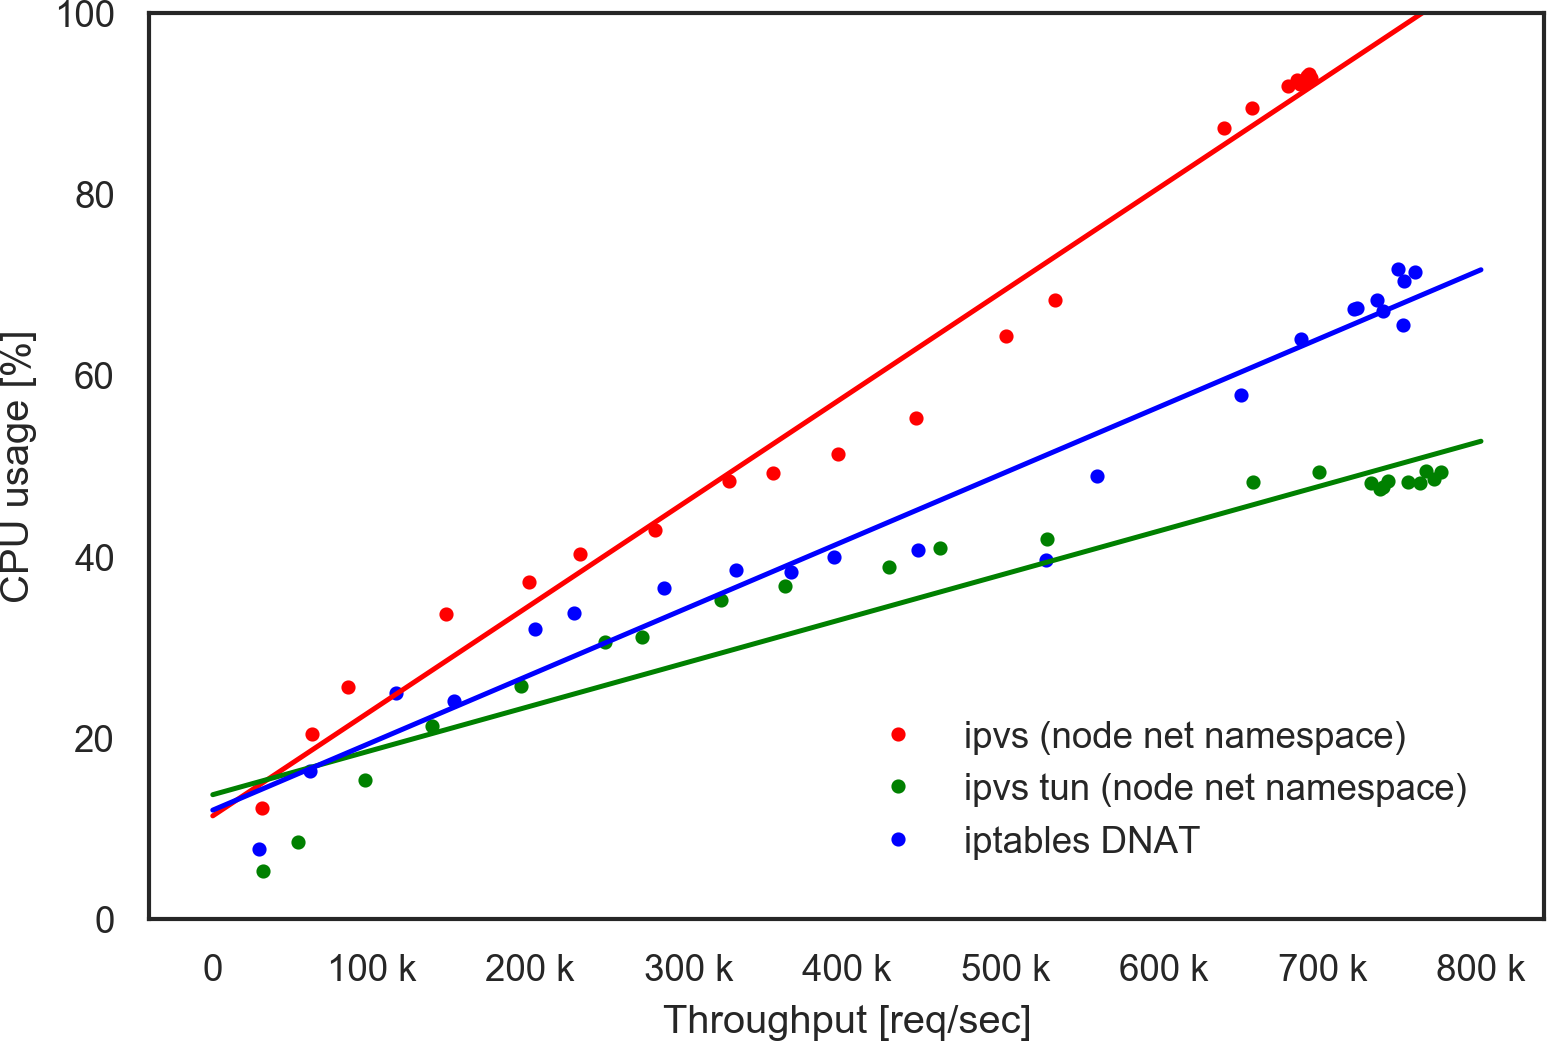
\includegraphics[width=0.8\columnwidth]{Figs/cpu_usage_10g_node_ns}
  \par\bigskip
  \centering
  \begin{minipage}{0.9\columnwidth}
    \caption[CPU usage of load balancers on nodes]{
      CPU usage of load balancers on nodes.
      CPU usages of ipvs and ipvs-tun greatly improved from those in Figure~\ref{fig:cpu_usage_10g} by placing them in node net namespace.  
      While the ipvs-tun consumes the smallest amount of the CPU resource, the CPU usage of ipvs is still larger than that of iptables DNAT.
    }
    \label{fig:cpu_usage_10g_node_ns}
  \end{minipage}
\end{figure}

The author summarizes this section as follows;
The ipvs itself is less efficient than iptables DNAT.
Using the container network, i.e., veth+bridge further degrades the throughput of ipvs.

\FloatBarrier

\section{Discussion of required throughput}

The author has compared the performance of proposed load balancers in 10Gbps in the previous section.
Although the proposed load balancer may not be the most efficient one, it is still useful because of the lateral scalability.

Table~\ref{tab:performance_summary} summarizes the maximum throughputs of the different load balancers obtained in the experiments so far.
Depending on the experimental conditions different part of the setup limits the throughput of the load balancers.
Since the performance bottlenecks are mainly due to network bandwidth in 1Gbps network, it is easy to estimate the possible bottleneck due to bandwidth in a faster network.
Since benchmark client exists at the location where normally the upstream router exists, the performance bottleneck at the benchmark client corresponds to the maximum throughput that the load balancer should handle..

For example, the bottleneck at the benchmark client is about 293K [req/sec] in the 1Gbps network. 
The load balancers only need to be able to handle at most 293K [req/sec] equivalent traffic.
Even if the load balacer is capable of handling 500K [req/sec], the throughput of the system is ultimately determined by the bottleneck at the entrance, that is 293K [req/sec].
The maximum throughput in 1Gbps, i.e., 293K [req/seq] is easily achieved by single ipvs-tun (293K [req/seq]) or two of ipvs load balancers (193K x 2 [req/seq]) with ECMP redundancy.

In the case of 10Gbps network, the maximum throughput determined by the bottleneck at the entrance is 2.9M [req/sec].
This is still easily achievable by using four of ipvs-tun (731K x 4 [req/seq]) or nine of ipvs load balancers (335K x 9 [req/seq]) with ECMP redundancy.

In the case of 100Gbps network, where the load balancers are required to accommodate up to throughput of 29M [req/sec], the inefficiency of the software load balancer in a container can become a real problem.
Because in order to handle 29M [req/sec] of the traffic, 90 of ipvs load balancer will be needed.
In the next section, the author tries to improve the efficiency of a load balancer, by implementing novel XDP load balancer.

\begin{table}[h]

  \begin{subtable}{1\textwidth}
    \centering
    \begin{tabular}{|l|l|c|l|}
      \hline
      \multicolumn{1}{|c|}{Type} & \multicolumn{1}{c|}{namespace} &
      \begin{tabular}{c} Throughput \\ {[}req/sec{]} \end{tabular} & \multicolumn{1}{c|}{Bottleneck} \\ \hline
      iptables DNAT & node      & 193K &
      \begin{tabular}{l} Bandwidth filled with request \\ + response @ load balancer \end{tabular} \\ \hline
      ipvs          & container & 197K &
      \begin{tabular}{l} Bandwidth filled with request \\ + response @ load balancer \end{tabular} \\ \hline
      ipvs-tun      & container & 293K &
      \begin{tabular}{l} Bandwidth filled with response \\ @ benchmark client  \end{tabular} \\ \hline
    \end{tabular}
    \caption{1Gbps experiment}
  \end{subtable}

  \par\bigskip

  \begin{subtable}{1\textwidth}
    \centering
    \begin{tabular}{|l|l|c|l|}
      \hline
      \multicolumn{1}{|c|}{Type} & \multicolumn{1}{c|}{namespace} &
      \begin{tabular}{c} Throughput \\ {[}req/sec{]} \end{tabular} & \multicolumn{1}{c|}{Bottleneck} \\ \hline
      iptables DNAT & node      & 778K & \begin{tabular}{l} CPU\(\sim\)100\% @ benchmark client\end{tabular} \\ \hline
      ipvs          & container & 335K & \begin{tabular}{l} CPU\(\sim\)100\% @ load balancer node\end{tabular} \\ \hline
        ipvs-tun      & container & 731K & \begin{tabular}{l} CPU\(\sim\)100\% @ load balancer node\end{tabular} \\ \hline
          ipvs          & node      & 700K & \begin{tabular}{l} CPU\(\sim\)100\% @ load balancer node\end{tabular} \\ \hline
      ipvs-tun      & node      & 780K & \begin{tabular}{l} CPU\(\sim\)100\% @ benchmark client\end{tabular} \\ \hline
   \end{tabular}
      \caption{10Gbps experiment}
  \end{subtable}

  \par\bigskip
  \centering
  \begin{minipage}{0.9\columnwidth}
    \caption[Summary of the maximum throughputs]{
      Summary of the maximum throughputs.
    }
    \label{tab:performance_summary}
  \end{minipage}
\end{table}

\FloatBarrier

\section{XDP load balancer}

The eXpress Data Path(XDP) is Linux kernel technology recently developed, where the tools and functionality to incept and process the packets in the earlist phase as possible are provided.
By utilizing XDP, one can hook a byte-compiled code developed in subset of the C programing language, to a place before the socket buffer is assigned, thereby speeding up network manupulation, including block against DDOS atack, simple packet forwarding and load balancing.
The one of the benefit of the XDP compared to DPDK is that in the case XDP, the packtes that do not match the rule for processing are then passd to normal Linux network stack.
Therefore there is no need for preparing dedicated NIC for fast and efficient network processing.
The author implemented the XDP load balacer and carried out throughput measurement.

\subsubsection{Implementation}

\subsubsection{Benchmark setup}

\subsubsection{Throughput results }

The author carried out the throughput measurement for the XDP load balacer, xlb.
The hardware and software configuretions are same as the ones in Table~\ref{tab:hw_sw_spec_10g}.
The exprimental setup is also same as the one in Figure~\ref{fig:benchmark-schem-10g}(b).
Since current implementation of xlb does not support multi core packet processing, the setting \enquote{(RSS,RPS)=(off,off)} is used in the throughput measurement.
All the intterrupt from the NIC are notified to a single core.

Figure~\ref{fig:cpu_usage_10g_xlb} compares the throughput of xlb and iptables DNAT. 
Although a single core is used for the packet processing, the throughput of the xlb load balancer is close to half of the iptables DNAT's throughput with 16 core(eight physical cores) packet processing.
Figure\ref{fig:cpu_usage_10g_xlb} compares CPU usages between xlb and iptables DNAT.
At a given throughput the xlb consumes much less CPU resource than iptables DNAT.
These results indicate that load balancer using XDP technology is very promising.

\begin{figure}[h]
  \centering
  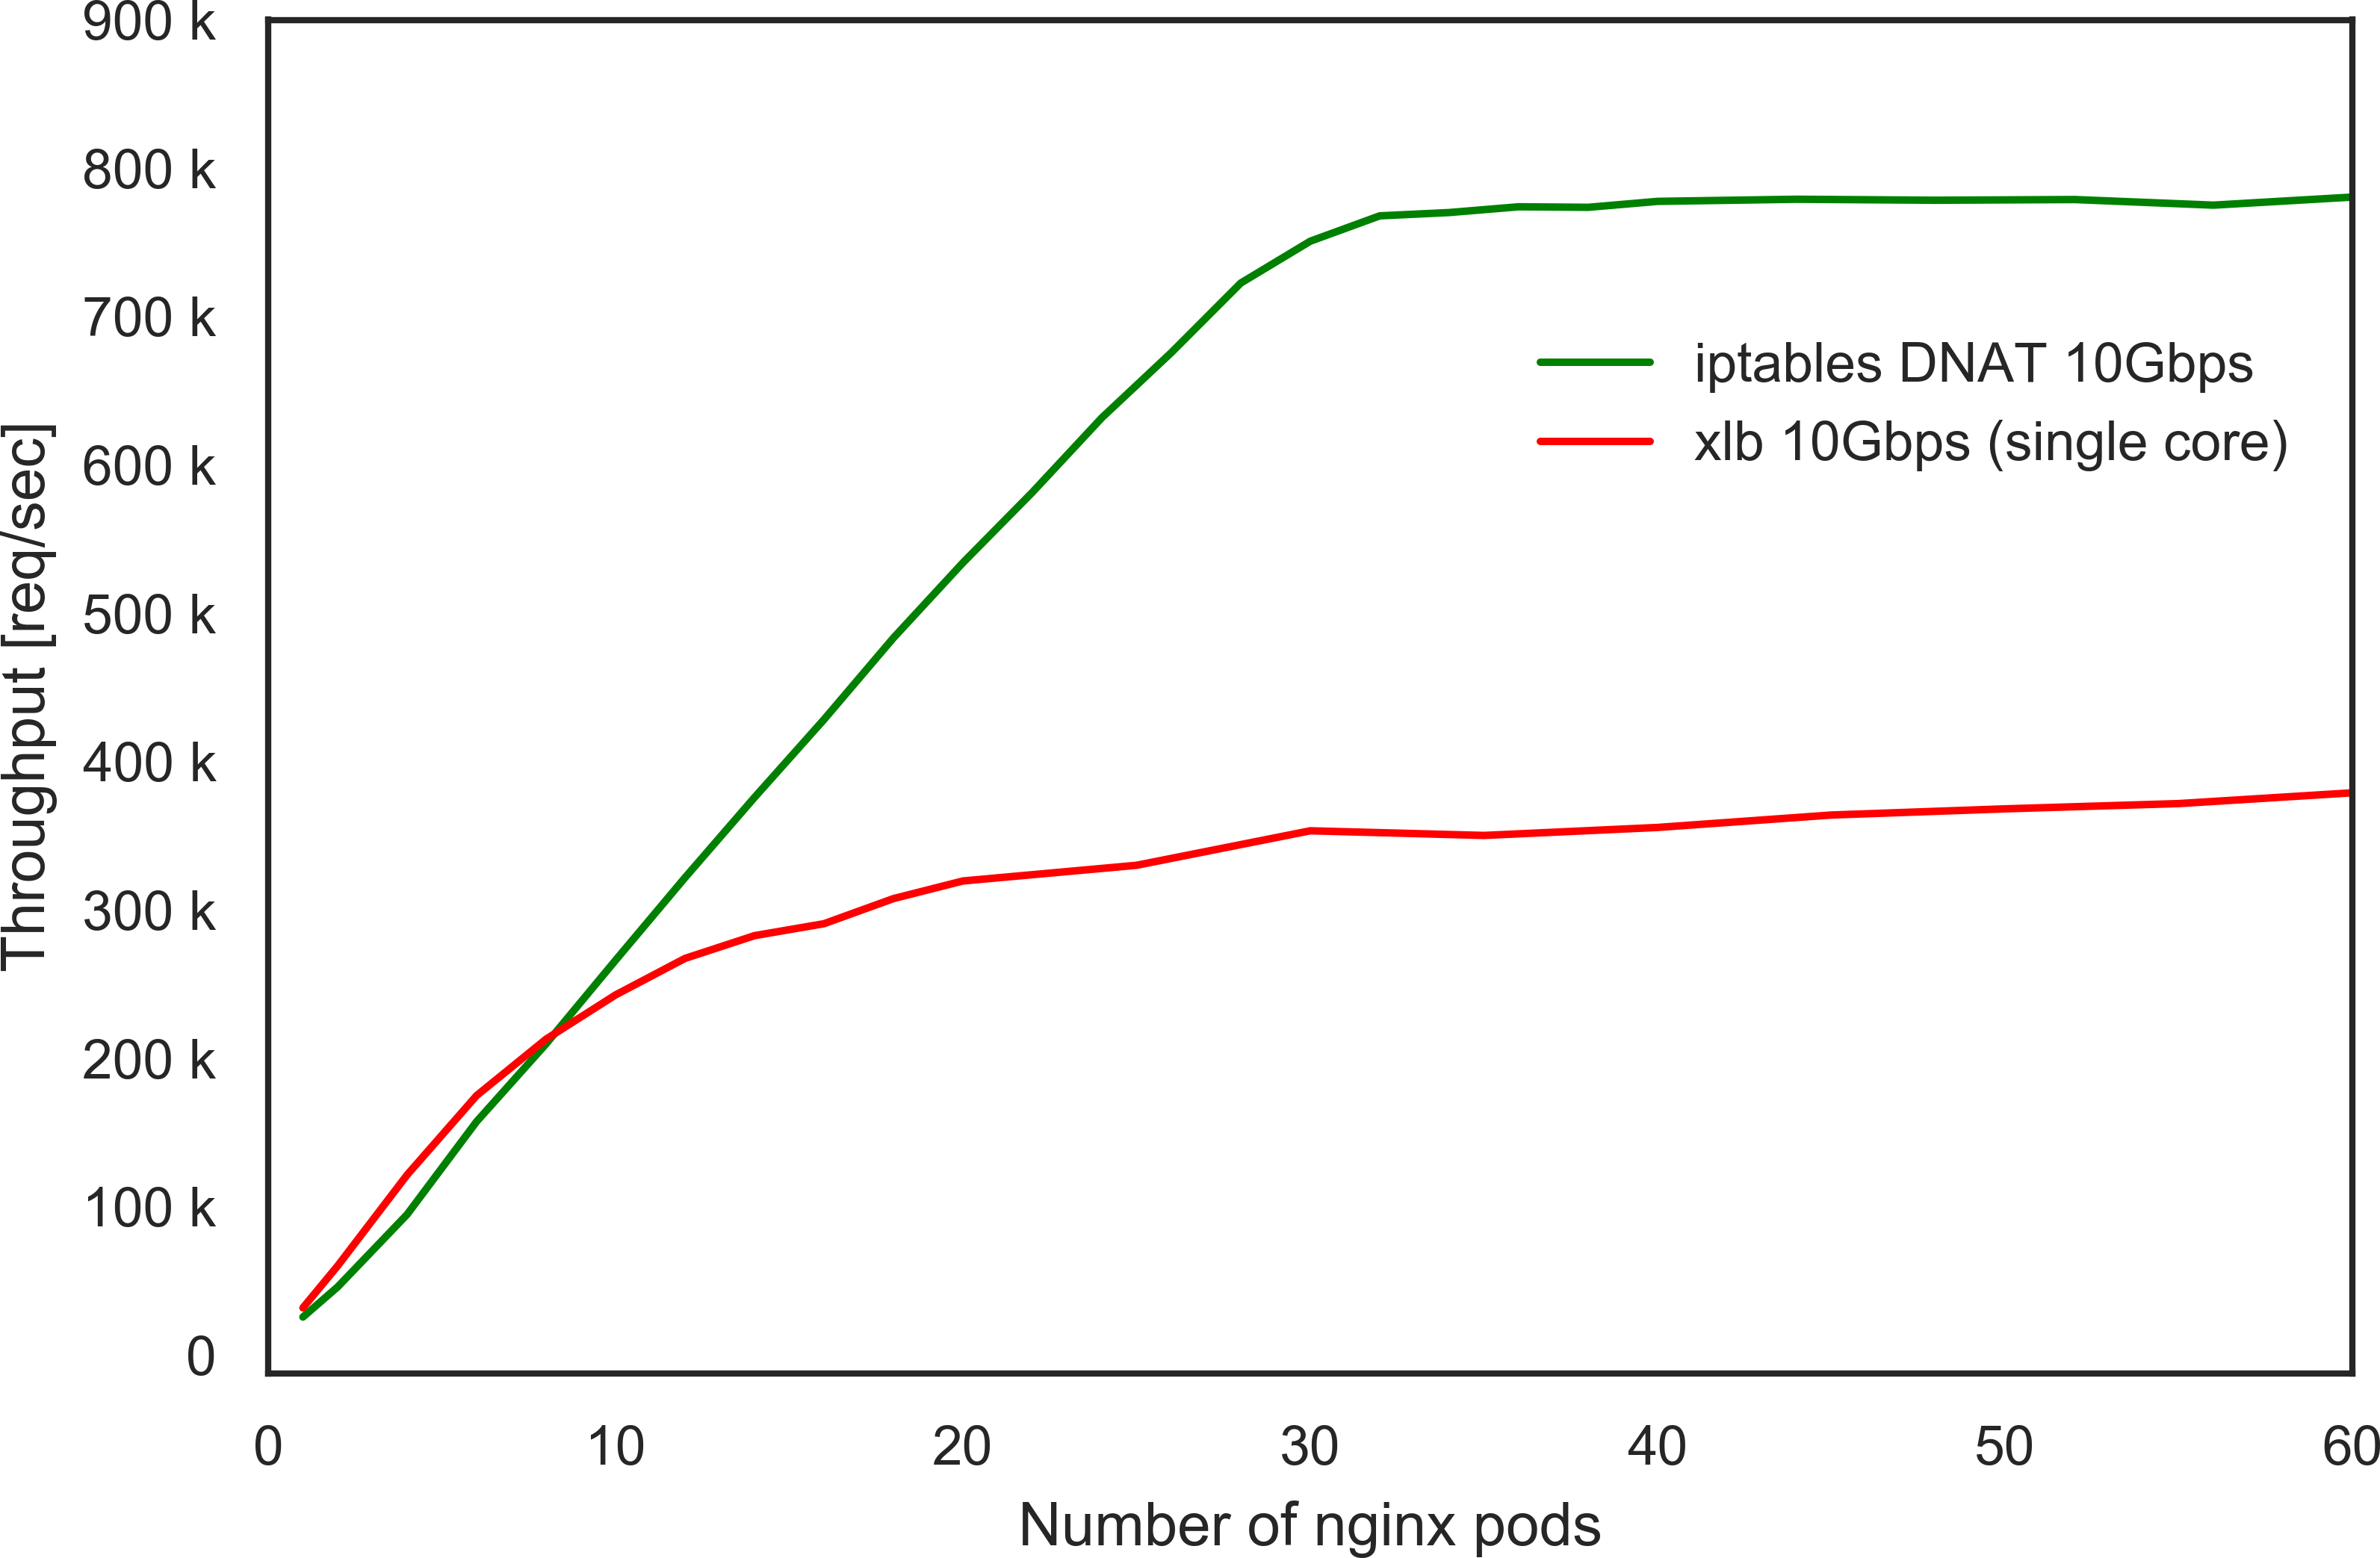
\includegraphics[width=0.8\columnwidth]{Figs/xlb_iptables_dnat_10g}
  \par\bigskip
  \centering
  \begin{minipage}{0.9\columnwidth}
    \caption[Throughput of xlb load balancer]{
      Throughput of xlb load balancer.
      The xlb load balancer is placed in node net namespace.
      The setting \enquote{(RSS,RPS)=(off,off)}, i.e., single core packet processing is used for the xlb measurement.
      The results of iptables DNAT for \enquote{(RSS,RPS)=(on,off)} and \enquote{(RSS,RPS)=(off,off)} are also shown for comparison.
      The throughput of the xlb is much higher than that of iptables DNAT with single core packet processing.
      Although using only a single core for, the throughput of the xlb load balancer is close to half of the iptables DNAT's with 16 core(eight physical corex) pakcet processing.
    }
    \label{fig:xlb_iptables_dnat_10g}
  \end{minipage}
\end{figure}


\begin{figure}[h]
  \centering
  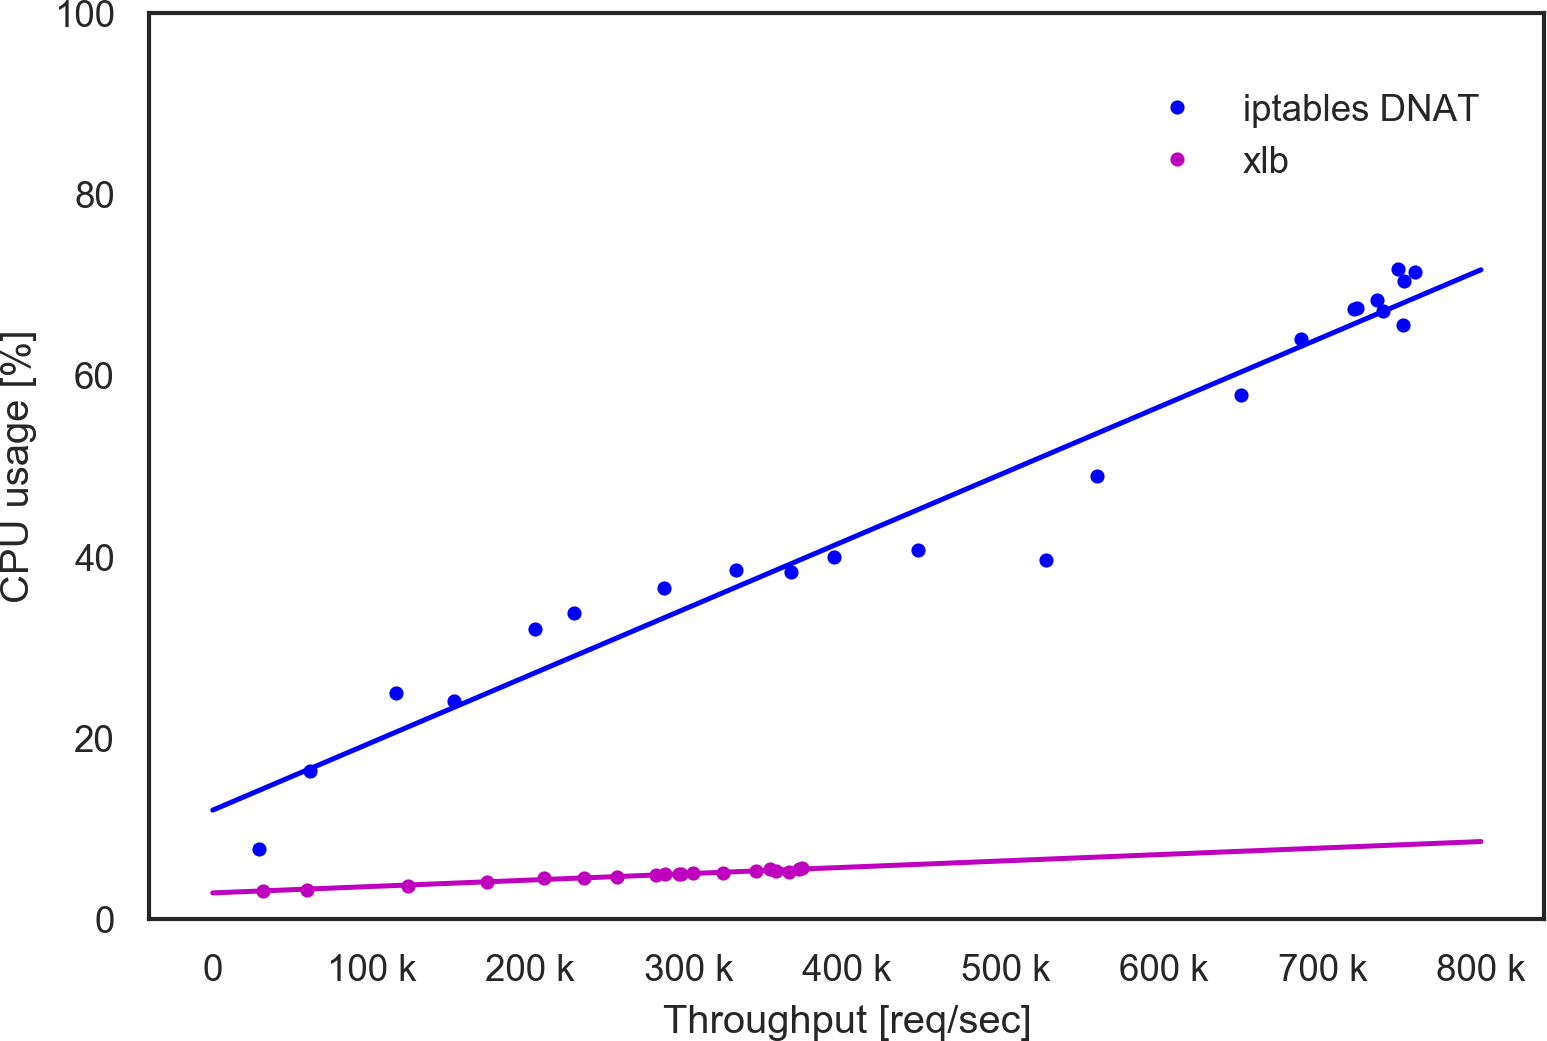
\includegraphics[width=0.8\columnwidth]{Figs/cpu_usage_10g_xlb}
  \par\bigskip
  \centering
  \begin{minipage}{0.9\columnwidth}
    \caption[CPU usage of xlb load balancer]{
      CPU usage of xlb load balancer.
      The xlb uses much less CPU resource than iptables DNAT.
    }
    \label{fig:cpu_usage_10g_xlb}
  \end{minipage}
\end{figure}

\FloatBarrier

\section{Summary}

In this chapter, the author carried out throughput measurements of ipvs, ipvs-tun, and iptables DNAT in 10Gbps environment.
From the results, the general characteristics of a load balancer are observesd.
The throughputs of ipvst and ipvs-tun are smaller than that of iptables DNAT in 10Gbps network, both due to the overhead of the container network and inefficiency in the program itself.
In order to improve the performance levels of portable load balancer, better network setup for containers and more efficient load balancer software should be developed.

However, considering the fact that the ultimate throughput of the system does not exceed that of the upstream router, the entrance, 
the load balancers only need to be able to handle at most 293K, 2.9M, and 29M [req/sec], in 1Gbps, 10Gbps, and 100Gbps, respectively.
Since a single ipvs in container can handle 335K [req/sec], traffic equivalent to 2.9M [req/sec], which is the maximum throughput achievable in 10Gbps, can be easily handled by nine of ipvs containers.

The author also presented the priliminary result of xlb experiment, which will be needed in 100Gbps network environment.
The obtained per core throughput result and CPU usage result have been very promising.



\chapter{Related Work}\label{chapter:Related Work}

This Chapter provides related work of this study.

\section{Related Work}\label{Related Work}

This section highlights related work, especially that dealing with container cluster migration, 
software load balancer containerization, load balancer tools within the context of the container technology and scalable load balancer in the cloud providers.

\paragraph{\bf Container cluster migration:}

Kubernetes developers are trying to add federation\cite{K8sFederation2017} capability for handling situations 
where multiple Kubernetes clusters\footnote{The {\em Kubernetes cluster} refers to a server cluster 
controlled by the Kubernetes container management system, in this paper.} 
are deployed on multiple cloud providers or on-premise data centers, 
and are managed via the Kubernetes federation API server (federation-apiserver). 
However, how each Kubernetes cluster is run on different types of cloud providers
and/or on-premise data centers, especially when the load balancers of such environments are not supported by Kubernetes, 
seems beyond the scope of that project. 
The main scope of this paper is to make Kubernetes usable in environments 
without supported load balancers by providing a containerized software load balancer.

\paragraph{\bf Software load balancer containerization:}
As far as load balancer containerization is concerned, the following related work has been identified:
Nginx-ingress\cite{Pleshakov2016,NginxInc2016} utilizes the ingress\cite{K8sIngress2017} capability of Kubernetes, 
to implement a containerized Nginx proxy as a load balancer. Nginx itself is famous as a high-performance web server program
that also has the functionality of a Layer-7 load balancer. Nginx is capable of handling Transport Layer Security(TLS) encryption, 
as well as Uniform Resource Identifier(URI) based switching. However, the flip side of Nginx is that it is much slower than Layer-4 switching.
We compared the performance between Nginx as a load balancer and our proposed load balancer in this paper.
%
Meanwhile, the kube-keepalived-vip\cite{Prashanth2016} project is trying to use Linux kernel's ipvs\cite{Zhang2000} 
load balancer capabilities by containerizing the keepalived\cite{ACassen2016}.
The kernel ipvs function is set up in the host OS's net namespaces and is shared among multiple web services,
as if it is part of the Kubernetes cluster infrastructure.
Our approach differs in that the ipvs rules are set up in container's net namespaces 
and function as a part of the web service container cluster itself.
The load balancers are configurable one by one, and are  movable with the cluster once the migration is needed.
The kube-keepalived-vip's approach lacks flexibility and portability whereas ours provide them.
%
The swarm mode of the Docker\cite{DockerCoreEngineering2016,DockerInc2017} also uses ipvs for internal load balancing,
but it is also considered as part of Docker swarm infrastructure, 
and thus lacks the portability that our proposal aims to provide.

\paragraph{\bf Load balancer tools in the container context:}
There are several other projects where efforts have been made to utilize ipvs in the context of container environment.
For example, GORB\cite{Sibiryov2015} and clusterf\cite{Aaltodoc:http://urn.fi/URN:NBN:fi:aalto-201611025433} are daemons 
that setup ipvs rules in the kernel inside the Docker container. 
They utilize running container information stored in key-value storages
like Core OS etcd\cite{CoreOSEtcd} and HashiCorp's Consul\cite{HashiCorpConsul}. 
Although these were usable to implement a containerized load balancer in our proposal, we did not use them, 
since Kubernetes ingress framework already provided the methods to retrieve running container information through standard API.

\paragraph{\bf Cloud load balancers:}

As far as the cloud load balancers are concerned, two articles have been identified.
Google's Maglev\cite{eisenbud2016maglev} is a software load balancer used in Google Cloud Platform(GCP).
Maglev uses modern technologies including per flow ECMP and kernel bypass for user space packet processing.
Maglev serves as the GCP's load balancer that is used by the Kubernetes.
Maglev is not a product that users can use outside of GCP nor is an open source software, while the users need open source software load balancer that is runnable even in on-premise data centers.
Microsoft's Ananta\cite{patel2013ananta} is another software load balancer implementation using ECMP and windows network stack.
Ananta can be solely used in Microsoft's Azure cloud infrastructure\cite{patel2013ananta}.
The proposed load balancer by the author is different in that it is aimed to be used in every cloud provider and on-premise data centers.




\cite{pellegrini2017preventing} "Preventing vendor lock-ins via an interoperable multi-cloud deployment approach"

\cite{felter2015updated} "An updated performance comparison of virtual machines and Linux containers"


\chapter{Conclusion}\label{chapter:Conclusion and future work}
\section{Conclusions}\label{Conclusions}

In this dissertation, the author proposed a portable load balancer with ECMP redundancy for the Kubernetes cluster systems that is aimed at facilitating migration of container clusters for web services.
The author implemented a containerized software load balancer that is run by Kubernetes as a part of container cluster, using Linux kernel's IPVS, as a proof of concept.
In order to discuss the feasibility of the proposed load balancer, we built 
a Kubernetes cluster system and conducted performance measurements.
Our experimental results indicate that the IPVS based load balancer in container improves the portability of 
the Kubernetes cluster system while it shows the similar performance levels as the existing iptables DNAT based load balancer.
We also clarified that choosing the appropriate operating modes of overlay networks is important for the performance of load balancers. 
For example, in the case of flannel, only the vxlan and udp backend operation modes could be used 
in the cloud environment, and the udp backend significantly degraded their performance.
Furthermore, we also learned that the distribution of packet processing among multiple CPUs was very important
to obtain the maximum performance levels from load balancers.

The throughput levels of a load balancer are dependent on settings for multicore packet processing.
It has been better to use as many CPU cores as possible for packet processing.
The throughput levels are also very dependent on the back end mode of the flannel overlay network.
The host-gw mode where no tunneling is used resulted in the best performance level.
It is clear that the case that utilizes all of the CPU cores better performs than the case with only four CPU cores utilized.
The performance levels of ipvs(nat), iptables DNAT and nginx have also been compared.
The proposed ipvs(nat) load balancer in the container had the same performance level as load balancing function of iptables DNAT.
Furthermore in the case of L3DSR setup, the performance level of ipvs(tun) load balancer has about 1.5 times larger that that of ipvs(nat) and iptables DNAT.
It is also shown that the proposed load balancer can be run in GCP and AWS.
The behavior of the proposed load balancer in those cloud environments is the same as that in the on-premise data center.
The author conclude that the proposed load balancer is portable and performs at the same level as the existing load balancers.


The ECMP technique is expected to make the load balancers redundant and scalable since all the load balancer containers act as active.
The whole system is resilient to a single failure of load balancer container.
Also since multiple of load balancers can be utilized simultaneously, it is expected that the throughput of the total system is increased significantly.
In order to evaluate these characteristics of the ECMP technique,
the author examined if the ECMP routing table is updated correctly when multiple of the load balancer {\em pods} are started.
After that, in order to explore the scalability, the author also measured the throughput of the cluster of load balancers.
Finally, the author examined how quick those ECMP routing table updates are.
The author verified that ECMP routing table was properly created in the experimental system.
The update of the ECMP routing table was correct and quick enough, i.e., within 10 seconds, throughout 20 hours experiment.
The scalability of the load balancer was also examined and it has been found that maximum performance levels scaled linearly as the number of the load balancer pods was increased to four.
The maximum throughput level obtained through the experiment was 780k [req/sec], which is limited due to the maximum CPU performance of the benchmark client rather than the performance of the load balancer cluster.

%

The limitations of this work that authors aware of include the followings: 
2) Experiments are conducted only in a 1Gbps network environment.
The experimental results indicate the performance of IPVS may be limited by the network bandwidth, 1Gbps, in our experiments. 
Thus, experiments with the faster network setting, e.g. 10Gigabit ethernet, are needed to investigate the feasibility of the proposed load balancer.



%\chapter{Conclusion and future work}\label{chapter:Conclusion and future work}
%[Filled in later]

%% The current limitations of this study are; 
%% 1) Although our proposed architecture is feasible where users can set up iBGP peer connections to upstream routers, currently major cloud providers do not seem to provide such services.
%% 2) ...
%% These should be addressed in the future work.
%% For other future work we plan to improve performance of a single software load balancer on standard Linux box using Xpress Data Plane(XDP) technology. 

Although major cloud providers do not currently provide BGP peering service for their users, the authors expect our proposed load balancer will be able to run, once this approach is proven to be beneficial and they start BGP peering services.
Therefore we focus our discussions on verifying that our proposed load balancer architecture is feasible, at least in on-premise data centers.
For the cloud environment without BGP peering service, single instance of ipvs load balancer can still be run with redundancy.
The liveness of the load balancer is constantly checked by one of the Kubernetes agents, and if anything that stop the load balancer happens, Kubernetes will restart the load balancer container.
The routing table of the cloud provider can be updated by newly started ipvs container immediately.

The authors limit the focus of this study on providing a portable load balancer for Kubernetes to prove the concept of proposed architecture.
However, the same concept can be easily applied to other container management systems, which should be discussed in future work.






%-----------------------------------------------------------

% =====================================================
%  Back Matter
% =====================================================

%\backmatter


% =====================================================
%  Bibliography
% =====================================================

%\bibliographystyle{plain}
\bibliographystyle{unsrt}
\bibliography{Bib/reference}


% =====================================================
%  Appendices
% =====================================================

\begin{appendices}


\chapter{ingress controller}
%\section{ingress controller}
\label{appendix:ingress_controller}

\begin{lstlisting}[
    basicstyle=\footnotesize,
    breaklines=true,
    postbreak=\mbox{\textcolor{red}{$\hookrightarrow$}\space},
  ]
package main

import (
	"log"
	"net/http"
	"os"
	"syscall"
	"os/exec"
	"strings"
	"text/template"
	"github.com/spf13/pflag"
	api "k8s.io/client-go/pkg/api/v1"
	nginxconfig "k8s.io/ingress/controllers/nginx/pkg/config"
	"k8s.io/ingress/core/pkg/ingress"
	"k8s.io/ingress/core/pkg/ingress/controller"
	"k8s.io/ingress/core/pkg/ingress/defaults"
)

var cmd = exec.Command("keepalived", "-nCDlf", "/etc/keepalived/ipvs.conf")

func main() {
	ipvs := newIPVSController()
	ic := controller.NewIngressController(ipvs)
	cmd.Stdout = os.Stdout
	cmd.Stderr = os.Stderr
	cmd.Start()
	defer func() {
		log.Printf("Shutting down ingress controller...")
		ic.Stop()
	}()
	ic.Start()
}

func newIPVSController() ingress.Controller {
	return &IPVSController{}
}

type IPVSController struct{}

func (ipvs IPVSController) SetConfig(cfgMap *api.ConfigMap) {
	log.Printf("Config map %+v", cfgMap)
}

func (ipvs IPVSController) Reload(data []byte) ([]byte, bool, error) {
	cmd.Process.Signal(syscall.SIGHUP)
	out, err := exec.Command("echo", string(data)).CombinedOutput()
	if err != nil {
		return out, false, err
	}
	log.Printf("Issue kill to keepalived. Reloaded new config %s", out)
	return out, true, err
}

func (ipvs IPVSController) OnUpdate(updatePayload ingress.Configuration) ([]byte, error) {
	log.Printf("Received OnUpdate notification")
	for _, b := range updatePayload.Backends {
		type ep struct{
			Address,Port string
		}
		eps := []ep{}
		for _, e := range b.Endpoints {
			eps = append(eps, ep{Address: e.Address, Port: e.Port})
		}

		for _, a := range eps {
		log.Printf("Endpoint %v:%v added to %v:%v.", a.Address, a.Port, b.Name, b.Port)
		}

		if b.Name == "upstream-default-backend" {
			continue
		}
		cnf := []string{"/etc/keepalived/ipvs.d/" , b.Name , ".conf"}
		w, err := os.Create(strings.Join(cnf, ""))
		if err != nil {
			return []byte("Ooops"), err
		}
		tpl := template.Must(template.ParseFiles("ipvs.conf.tmpl"))
		tpl.Execute(w, eps)
		w.Close()
	}
	
	return []byte("hello"), nil
}

func (ipvs IPVSController) BackendDefaults() defaults.Backend {
	// Just adopt nginx's default backend config
	return nginxconfig.NewDefault().Backend
}

func (ipvs IPVSController) Name() string {
	return "IPVS Controller"
}

func (ipvs IPVSController) Check(_ *http.Request) error {
	return nil
}

func (ipvs IPVSController) Info() *ingress.BackendInfo {
	return &ingress.BackendInfo{
		Name:       "dummy",
		Release:    "0.0.0",
		Build:      "git-00000000",
		Repository: "git://foo.bar.com",
	}
}

func (ipvs IPVSController) OverrideFlags(*pflag.FlagSet) {
}

func (ipvs IPVSController) SetListers(lister ingress.StoreLister) {
}

func (ipvs IPVSController) DefaultIngressClass() string {
	return "ipvs"
}
\end{lstlisting}

\chapter{ECMP settings}
\section{Exabgp configuration on the load balancer container.}
\label{appendix:exabgp_config}

{\bf\normalsize exabgp.conf:}
\begin{verbatim}
neighbor 10.0.0.109 {
 description "peer1";
 router-id 172.16.20.2;
 local-address 172.16.20.2;
 local-as 65021;
 peer-as 65021;
 hold-time 1800;
   static {
     route 10.1.1.0/24 next-hop 10.0.0.106;
   }
}
\end{verbatim}

\section{Gobgpd configuration on the route reflector.}
\label{appendix:route_reflector_config}

{\bf\normalsize gobgp.conf:}
\begin{verbatim}
global:
  config:
    as: 65021
    router-id: 10.0.0.109
    local-address-list:
    - 0.0.0.0 # ipv4 only
  use-multiple-paths:
    config:
      enabled: true

peer-groups:
  - config:
      peer-group-name: k8s
      peer-as: 65021
    afi-safis:
      - config:
          afi-safi-name: ipv4-unicast

dynamic-neighbors:
  - config:
      prefix: 172.16.0.0/16
      peer-group: k8s

neighbors:
  - config:
      neighbor-address: 10.0.0.110
      peer-as: 65021
    route-reflector:
      config:
        route-reflector-client: true
        route-reflector-cluster-id: 10.0.0.109
    add-paths: 
      config:
        send-max: 255
        receive: true

\end{verbatim}

\section{Gobgpd and zebra configurations on the router.}

{\bf\normalsize gobgp.conf:}
\begin{verbatim}
global:
  config:
    as: 65021
    router-id: 10.0.0.110
    local-address-list:
    - 0.0.0.0

  use-multiple-paths:
    config:
      enabled: true

neighbors:
    - config:
        neighbor-address: 10.0.0.109
        peer-as: 65021
      add-paths:
        config:
          receive: true

zebra:
  config:
    enabled: true
    url: unix:/run/quagga/zserv.api
    version: 3
    redistribute-route-type-list: 
      - static

\end{verbatim}
\label{appendix:router_config}
%
{\bf\normalsize zebra.conf:}
\begin{verbatim}
hostname Router
log file /var/log/zebra.log
\end{verbatim}

%\caption{Example of zebra config on the router.}
%\label{fig:zebra_config_router}

\chapter{Analysis of the performance limit}
\label{appendix:performance_limit}

The maximum throghput in this series of experiment is roughly, 190k[req/sec] for both ipvs an the iptables DNAT.
At first, it was not clear what caused this limit.
The author analyzed the kind of packets that flows during the experiment using tcpdump\cite{jacobson1989tcpdump} as follows;
1) A wrk worker opens multiple connections and sends out http request to the web servers. The number of connections is determined by the command-line option, eg. 800/40 = 20 connection in the case of command-line in Table~\ref{tab:bench_example}. The worker sends out 100 requests to the web server within each connection, and closes it either if all of the responses are recieved or time out occurs.
2) As in seen in Listing~\ref{list:tcpdump}, tcp options were mss(4 byte), sack(2 byte), ts(10 byte), nop(1 byte) and wscale(3 byte), for SYN packets. For other packets, tcp options were, nop(1 byte), nop(1 byte) and ts(10 byte).
3) The author classified the types of packes and counted the number of each type in a single connection, which is 100 http requests. Table~\ref{tab:request_data_size},\ref{tab:response_data_size},\ref{tab:header_size} summarize the data size of 100 request, including TCP headr, IP header, Ether header and overheads. 
From this analysis, it was found that per each HTTP request and response,
request data with the size of 227.68[byte] and response data with the data(http content)+437.68[byte] were being sent.   

Since the node for load balancer recives and transmits both request and response packets using single network interface, each 1Gbps half duplex of full duplex must accomodate request and response data size.
Therefore the theoretical maximum throughput can be expressed as; \\
throughput[req/sec] = band width[byte/sec]/(request + response) \\
= 1e9/8/(data+665.36)

Figure~\ref{fig:performance_limit} shows plot of theoretical maximum throughput 1Gbps ethernet together with actual benchmark results.
Since experimnetal results agrees well with theory, the author concludes that when \enquote{RPS = on}, ipvs performance limit is due to the 1Gbps bandwidth.

\begin{lstlisting}[
    backgroundcolor = \color{mygray},
    basicstyle=\footnotesize,
    breaklines=true,
    numbers=left,
    %    postbreak=\mbox{\textcolor{red}{$\hookrightarrow$}\space},
    caption={An example of the tcpdump output},
    captionpos=b,
    label={list:tcpdump}
  ]
  curl -s  http://172.16.72.2:8888/1000
  tcpdmup(response):

  03:09:27.968942 IP 172.16.72.2.8888 > 192.168.0.112.60142:
  Flags [S.], seq 2317920646, ack 648140715, win 28960, options [mss 1460,sackOK,TS val 2274012282 ecr 2324675546,nop,wscale 8], length 0
  03:09:27.969685 IP 172.16.72.2.8888 > 192.168.0.112.60142:
  Flags [.], ack 85, win 114, options [nop,nop,TS val 2274012282 ecr 2324675546], length 0
  03:09:27.969945 IP 172.16.72.2.8888 > 192.168.0.112.60142:
  Flags [P.], seq 1:255, ack 85, win 114, options [nop,nop,TS val 2274012282 ecr 2324675546], length 254
  03:09:27.969948 IP 172.16.72.2.8888 > 192.168.0.112.60142:
  Flags [P.], seq 255:1255, ack 85, win 114, options [nop,nop,TS val 2274012282 ecr 2324675546], length 1000
  03:09:27.970846 IP 172.16.72.2.8888 > 192.168.0.112.60142:
  Flags [F.], seq 1255, ack 86, win 114, options [nop,nop,TS val 2274012282 ecr 2324675547], length 0
\end{lstlisting}

\begin{table}[h]
\centering
  \begin{tabular}{|l|r|r|r|r|}
    \hline
%    \multicolumn{5}{|l|}{Data size in 100 HTTP requests.} \\ \hline
    Type of Packet & \multicolumn{1}{l|}{Payload {[}byte{]}} & \multicolumn{1}{l|}{Header {[}byte{]}} & \multicolumn{1}{l|}{Count} & \multicolumn{1}{l|}{Total {[}byte{]}} \\ \hline
    SYN & 0 & 98 & 1 & 98 \\ \hline
    ACK & 0 & 90 & 102 & 9,180 \\ \hline
    Push(GET) & 44 & 90 & 100 & 13,400 \\ \hline
    FIN+ACK & 0 & 90 & 1 & 90 \\ \hline
    \multicolumn{3}{|l|}{Total} & \multicolumn{2}{r|}{22,768} \\ \hline
  \end{tabular}
  \caption{Request data size for 100 HTTP requests in wrk measurement.}
  \label{tab:request_data_size}
%% \end{table}

  \vspace{1cm}
  
%% \begin{table}[h]
\centering
  \begin{tabular}{|l|r|r|r|r|}
    \hline
%    \multicolumn{5}{|l|}{Response Data size for 100 HTTP requests in wrk measurement.} \\ \hline
    Type of Packet & \multicolumn{1}{l|}{Payload {[}byte{]}} & \multicolumn{1}{l|}{Header {[}byte{]}} & \multicolumn{1}{l|}{Count} & \multicolumn{1}{l|}{Total {[}byte{]}} \\ \hline
    SYN+ACK & 0 & 98 & 1 & 98 \\ \hline
    ACK & 0 & 90 & 2 & 180 \\ \hline
    Push(GET) & 254 & 90 & 100 & 34,400 \\ \hline
    Push(DATA) & data & 90 & 100 & 100x(data+90) \\ \hline
    FIN+ACK & 0 & 90 & 1 & 90 \\ \hline
    \multicolumn{3}{|l|}{Total} & \multicolumn{2}{r|}{100x(data+90)+34,768} \\ \hline
  \end{tabular}
  \caption{Response data size for 100 HTTP requests in wrk measurement.}
  \label{tab:response_data_size}
\end{table}

\begin{table}[h]
\begin{center}
  \begin{tabular}{|l|r|r|}
    \hline
    Type of field & \multicolumn{1}{l|}{SYN} & \multicolumn{1}{l|}{\begin{tabular}[c]{@{}l@{}}ACK, SYN+ACK,\\ FIN+ACK, PUSH\end{tabular}} \\ \hline
    preamble & 8 & 8 \\ \hline
    ether header & 14 & 14 \\ \hline
    ip header & 20 & 20 \\ \hline
    tcp header & 20 + 20(tcp options) & 20 + 12(tcp options) \\ \hline
    fcs & 4 & 4 \\ \hline
    inter frame gap & 12 & 12 \\ \hline
    Total [byte] & 98 & 90 \\ \hline
  \end{tabular}
  \caption{Header sizes of TCP/IP packet in Ethernet frame.}
  \label{tab:header_size}
\end{center}
\end{table}



\end{appendices}


\end{document}
